\documentclass{article}
\PassOptionsToPackage{table}{xcolor}
\usepackage{iclr2027,times}

\input{math_commands.tex}

\usepackage{amsmath}
\usepackage{amssymb}
\usepackage{array}
\usepackage{booktabs}
\usepackage{caption}
\usepackage{enumitem}
\usepackage{graphicx}
\usepackage{hyperref}
\hypersetup{hidelinks}
\usepackage{multirow}
\usepackage{url}
\usepackage{wrapfig}
\usepackage{float}
\usepackage{placeins}
\usepackage{tikz}
\usetikzlibrary{arrows.meta,positioning}
\newcolumntype{L}[1]{>{\raggedright\arraybackslash}p{#1}}
\newcolumntype{C}[1]{>{\centering\arraybackslash}p{#1}}
\newcommand{\rev}[1]{#1}
\newcommand{\bestnum}[1]{\textbf{#1}}
\newcommand{\secondnum}[1]{\underline{#1}}
\newcommand{\thirdnum}[1]{\emph{#1}}
\newcommand{\bestcell}[1]{\textbf{#1}}
\newcommand{\secondcell}[1]{\underline{#1}}
\newcommand{\thirdcell}[1]{\emph{#1}}
\newcommand{\rotcls}[1]{\rotatebox{90}{\scriptsize #1}}

\definecolor{occBike}{RGB}{244,160,170}
\definecolor{occBus}{RGB}{241,120,52}
\definecolor{occCar}{RGB}{31,144,224}
\definecolor{occMotor}{RGB}{188,165,0}
\definecolor{occPed}{RGB}{226,35,35}
\definecolor{occTruck}{RGB}{153,78,24}
\definecolor{occOther}{RGB}{125,125,125}
\definecolor{occBarrier}{RGB}{96,62,45}
\definecolor{occCone}{RGB}{245,213,93}
\definecolor{occDrive}{RGB}{230,30,225}
\definecolor{occSide}{RGB}{85,21,91}
\definecolor{occTerrain}{RGB}{125,224,80}
\definecolor{occManmade}{RGB}{196,196,196}
\definecolor{occVegetation}{RGB}{0,185,0}
\definecolor{occFree}{RGB}{0,0,0}

\newcommand{\classswatch}[1]{\textcolor{#1}{\rule{0.70em}{0.70em}}}
\newcommand{\occclassname}[1]{\rotatebox{90}{\scriptsize #1}}
\newcommand{\occclasshead}[2]{%
  \begin{tabular}[b]{@{}c@{}}%
    \makebox[0.85em][c]{\rule{0pt}{6.4em}\rotatebox{90}{\scriptsize #2}}\\[-0.25ex]%
    \classswatch{#1}%
  \end{tabular}%
}
\newcommand{\modalityrow}[2]{%
  \rowcolor{gray!8}\multicolumn{#1}{@{}l}{\textbf{#2}}\\%
}
\newcommand{\pendingmethodrow}[2]{%
  #1~\cite{#2} & \multicolumn{19}{c}{\na} \\%
}


% \captionsetup{font=small}
\captionsetup[table]{skip=4pt}
% \setlength{\bibsep}{0pt}
\setlength{\textfloatsep}{8pt plus 2pt minus 2pt}
\setlength{\dbltextfloatsep}{8pt plus 2pt minus 2pt}
\setlength{\floatsep}{6pt plus 2pt minus 2pt}
\setlength{\intextsep}{6pt plus 2pt minus 2pt}
\newcommand{\method}{RoadOcc}
\newcommand{\figdir}{figures}
\newcommand{\best}[1]{\cellcolor{red!12}\textbf{#1}}
\newcommand{\todo}[1]{\textcolor{red}{\textit{#1}}}
\newcommand{\cmark}{\checkmark}
\newcommand{\xmark}{--}
\newcommand{\etal}{et al.\,}
\definecolor{hitmatch}{RGB}{64,176,64}
\definecolor{hitmismatch}{RGB}{220,55,55}
\definecolor{hitother}{RGB}{160,160,160}
\DeclareRobustCommand{\hitbox}[1]{%
  \raisebox{0.12ex}{\textcolor{#1}{\rule{1.0ex}{1.0ex}}}}

\newcommand{\motivationdiagram}{%
  \begingroup
  \setlength{\fboxsep}{4pt}
  \footnotesize
  \resizebox{\linewidth}{!}{%
    \begin{tabular}{@{}c@{\quad$\rightarrow$\quad}c@{\quad$\rightarrow$\quad}c@{\quad$\rightarrow$\quad}c@{}}
    \fcolorbox{gray}{gray!8}{\parbox[c][0.18in][c]{0.18\linewidth}{\centering Current\\dynamic object}} &
    \fcolorbox{red!65!black}{red!7}{\parbox[c][0.18in][c]{0.20\linewidth}{\centering Rigid history\\stale object location}} &
    \fcolorbox{orange!75!black}{orange!8}{\parbox[c][0.18in][c]{0.20\linewidth}{\centering Voxel velocity\\$\Delta t\,\widehat{\mathbf v}$}} &
    \fcolorbox{green!45!black}{green!7}{\parbox[c][0.18in][c]{0.20\linewidth}{\centering Retrieved history\\at current location}} \\
    \end{tabular}}
  \endgroup}

\newcommand{\roadoccdiagram}{%
  \begingroup
  \setlength{\fboxsep}{4pt}
  \footnotesize
  \resizebox{\linewidth}{!}{%
    \begin{tabular}{@{}c@{\quad$\rightarrow$\quad}c@{\quad$\rightarrow$\quad}c@{\quad$\rightarrow$\quad}c@{}}
    \fcolorbox{gray}{gray!8}{\parbox[c][0.47in][c]{0.18\linewidth}{\centering Four roadside\\camera views}} &
    \fcolorbox{blue!60!black}{blue!6}{\parbox[c][0.47in][c]{0.19\linewidth}{\centering Dynamic-aware\\Cross-attention (DCA)}} &
    \fcolorbox{orange!75!black}{orange!8}{\parbox[c][0.47in][c]{0.19\linewidth}{\centering Multi-scale Voxel\\Velocity Estimation (VVE)}} &
    \fcolorbox{green!45!black}{green!7}{\parbox[c][0.47in][c]{0.19\linewidth}{\centering Velocity-guided Dynamic\\Sparse Fusion (VDSF)}} \\
    \end{tabular}}
  \endgroup}

\newcommand{\velocitydiagram}{%
  \begingroup
  \setlength{\fboxsep}{3pt}
  \scriptsize
  \begin{tabular}{@{}c@{\hspace{0.015\linewidth}}c@{\hspace{0.015\linewidth}}c@{\hspace{0.015\linewidth}}c@{}}
  \fcolorbox{gray}{gray!8}{\parbox[c][0.42in][c]{0.21\linewidth}{\centering Current voxel state}} & $+$ &
  \fcolorbox{blue!60!black}{blue!6}{\parbox[c][0.42in][c]{0.21\linewidth}{\centering Aligned history\\local correspondence}} & $\rightarrow$ \\
  \multicolumn{3}{c}{} \\
  \multicolumn{3}{c}{\fcolorbox{orange!75!black}{orange!8}{\parbox[c][0.42in][c]{0.30\linewidth}{\centering VVE predicts planar velocity $\widehat{\mathbf v}_t(\mathbf x)$}}} & $\rightarrow$ \\
  \multicolumn{3}{c}{} \\
  \multicolumn{3}{c}{\fcolorbox{green!45!black}{green!7}{\parbox[c][0.42in][c]{0.34\linewidth}{\centering VDSF samples history at $\mathbf x-\Delta t\,\widehat{\mathbf v}_t(\mathbf x)$}}}
  \end{tabular}
  \endgroup}

\newcommand{\historydiagram}{%
  \begingroup
  \setlength{\fboxsep}{4pt}
  \footnotesize
  \resizebox{\linewidth}{!}{%
    \begin{tabular}{@{}c@{\quad$\rightarrow$\quad}c@{\quad$\rightarrow$\quad}c@{\quad$\rightarrow$\quad}c@{}}
    \fcolorbox{gray}{gray!8}{\parbox[c][0.52in][c]{0.20\linewidth}{\centering Historical voxel\\queue}} &
    \fcolorbox{blue!60!black}{blue!6}{\parbox[c][0.52in][c]{0.20\linewidth}{\centering Rigid coordinate\\alignment}} &
    \fcolorbox{orange!75!black}{orange!8}{\parbox[c][0.52in][c]{0.20\linewidth}{\centering VVE velocity\\sampling grid}} &
    \fcolorbox{green!45!black}{green!7}{\parbox[c][0.52in][c]{0.20\linewidth}{\centering VDSF residual\\fusion}} \\
    \end{tabular}}
  \endgroup}

\newcommand{\labeldiagram}{%
  \begingroup
  \setlength{\fboxsep}{3pt}
  \scriptsize
  \begin{tabular}{@{}c@{\hspace{0.02\linewidth}}c@{\hspace{0.02\linewidth}}c@{}}
    \fcolorbox{gray}{gray!8}{\parbox[c][0.48in][c]{0.25\linewidth}{\centering Dynamic box\\annotation}} & $\rightarrow$ &
    \fcolorbox{blue!60!black}{blue!6}{\parbox[c][0.48in][c]{0.25\linewidth}{\centering Voxel rasterization\\and temporal repair}} \\
    \multicolumn{3}{c}{\vspace{1pt}$\downarrow$} \\
    \fcolorbox{orange!75!black}{orange!8}{\parbox[c][0.48in][c]{0.25\linewidth}{\centering Multi-scale\\velocity target}} & $+$ &
    \fcolorbox{green!45!black}{green!7}{\parbox[c][0.48in][c]{0.25\linewidth}{\centering Semantic occupancy\\target}}
  \end{tabular}
  \endgroup}

\newcommand{\qualdiagram}{%
  \begingroup
  \setlength{\fboxsep}{4pt}
  \footnotesize
  \resizebox{\linewidth}{!}{%
    \begin{tabular}{@{}c@{\quad$\rightarrow$\quad}c@{\quad$\rightarrow$\quad}c@{\quad$\rightarrow$\quad}c@{}}
    \fcolorbox{gray}{gray!8}{\parbox[c][0.55in][c]{0.19\linewidth}{\centering Current semantic\\occupancy}} &
    \fcolorbox{blue!60!black}{blue!6}{\parbox[c][0.55in][c]{0.19\linewidth}{\centering Dynamic\\candidate support}} &
    \fcolorbox{orange!75!black}{orange!8}{\parbox[c][0.55in][c]{0.19\linewidth}{\centering Planar voxel\\velocity}} &
    \fcolorbox{green!45!black}{green!7}{\parbox[c][0.55in][c]{0.19\linewidth}{\centering Compensated\\historical evidence}} \\
    \end{tabular}}
  \endgroup}

\newcommand{\robustnessdiagram}{%
  \resizebox{.94\linewidth}{!}{%
  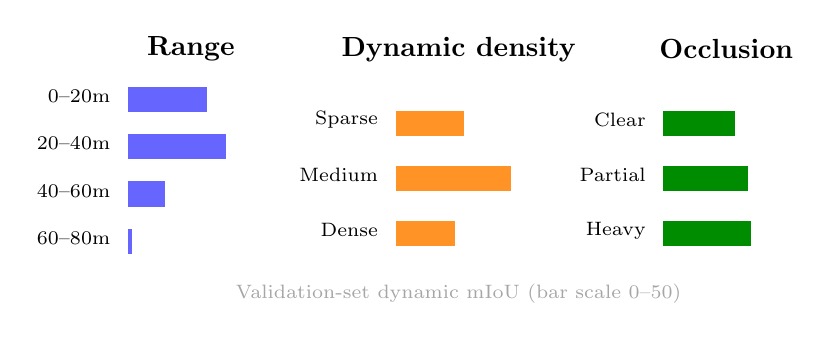
\begin{tikzpicture}[font=\scriptsize, >=Latex, line width=.4pt]
    \node[font=\bfseries] at (1.45,3.15) {Range};
    \node[font=\bfseries] at (4.85,3.15) {Dynamic density};
    \node[font=\bfseries] at (8.25,3.15) {Occlusion};
    \foreach \y/\label in {2.55/0--20,1.95/20--40,1.35/40--60,.75/60--80}
      \node[anchor=east] at (.55,\y) {\label m};
    \fill[blue!60] (.65,2.35) rectangle ++(1.00,.32);
    \fill[blue!60] (.65,1.75) rectangle ++(1.24,.32);
    \fill[blue!60] (.65,1.15) rectangle ++(.47,.32);
    \fill[blue!60] (.65,.55) rectangle ++(.05,.32);
    \foreach \y/\label in {2.25/Sparse,1.55/Medium,.85/Dense}
      \node[anchor=east] at (3.95,\y) {\label};
    \fill[orange!85] (4.05,2.05) rectangle ++(.87,.32);
    \fill[orange!85] (4.05,1.35) rectangle ++(1.47,.32);
    \fill[orange!85] (4.05,.65) rectangle ++(.76,.32);
    \foreach \y/\label in {2.25/Clear,1.55/Partial,.85/Heavy}
      \node[anchor=east] at (7.35,\y) {\label};
    \fill[green!55!black] (7.45,2.05) rectangle ++(.91,.32);
    \fill[green!55!black] (7.45,1.35) rectangle ++(1.08,.32);
    \fill[green!55!black] (7.45,.65) rectangle ++(1.11,.32);
    \node[text=gray!70,align=center] at (4.85,.05)
      {Validation-set dynamic mIoU (bar scale 0--50)};
  \end{tikzpicture}}}

\newcommand{\trajectorydiagram}{%
  \resizebox{\linewidth}{!}{%
  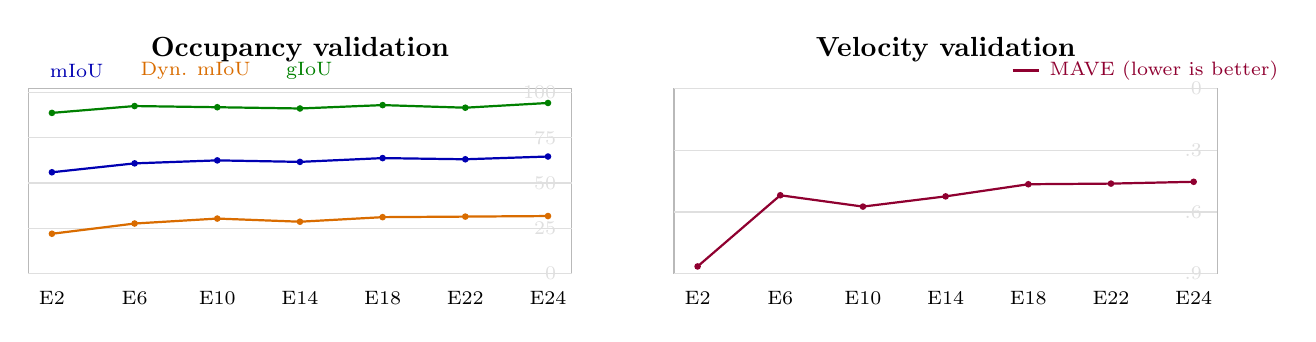
\begin{tikzpicture}[font=\scriptsize, >=Latex, line width=.45pt]
    \node[font=\bfseries] at (3.45,2.85) {Occupancy validation};
    \draw[gray!55] (0,0) rectangle (6.9,2.35);
    \foreach \y/\label in {0/0,.575/25,1.15/50,1.725/75,2.3/100}
      \draw[gray!25] (0,\y) -- (6.9,\y) node[anchor=east,xshift=-2pt] {\label};
    \foreach \x/\label in {.3/E2,1.35/E6,2.4/E10,3.45/E14,4.5/E18,5.55/E22,6.6/E24}
      \node[anchor=north] at (\x,-.10) {\label};
    \draw[blue!70!black,thick] plot coordinates {(.3,1.287) (1.35,1.400) (2.4,1.438) (3.45,1.419) (4.5,1.467) (5.55,1.452) (6.6,1.487)};
    \draw[orange!85!black,thick] plot coordinates {(.3,.506) (1.35,.636) (2.4,.699) (3.45,.659) (4.5,.717) (5.55,.724) (6.6,.731)};
    \draw[green!50!black,thick] plot coordinates {(.3,2.041) (1.35,2.128) (2.4,2.113) (3.45,2.097) (4.5,2.140) (5.55,2.107) (6.6,2.167)};
    \foreach \x/\y in {.3/1.287,1.35/1.400,2.4/1.438,3.45/1.419,4.5/1.467,5.55/1.452,6.6/1.487}
      \fill[blue!70!black] (\x,\y) circle (1.2pt);
    \foreach \x/\y in {.3/.506,1.35/.636,2.4/.699,3.45/.659,4.5/.717,5.55/.724,6.6/.731}
      \fill[orange!85!black] (\x,\y) circle (1.2pt);
    \foreach \x/\y in {.3/2.041,1.35/2.128,2.4/2.113,3.45/2.097,4.5/2.140,5.55/2.107,6.6/2.167}
      \fill[green!50!black] (\x,\y) circle (1.2pt);
    \node[anchor=west,text=blue!70!black] at (.15,2.58) {mIoU};
    \node[anchor=west,text=orange!85!black] at (1.30,2.58) {Dyn. mIoU};
    \node[anchor=west,text=green!50!black] at (3.15,2.58) {gIoU};
    \node[font=\bfseries] at (11.65,2.85) {Velocity validation};
    \draw[gray!55] (8.2,0) rectangle (15.1,2.35);
    \foreach \y/\label in {0/.9,.783/.6,1.567/.3,2.35/0}
      \draw[gray!25] (8.2,\y) -- (15.1,\y) node[anchor=east,xshift=-2pt] {\label};
    \foreach \x/\label in {8.5/E2,9.55/E6,10.6/E10,11.65/E14,12.7/E18,13.75/E22,14.8/E24}
      \node[anchor=north] at (\x,-.10) {\label};
    \draw[purple!75!black,thick] plot coordinates {(8.5,.091) (9.55,.995) (10.6,.851) (11.65,.981) (12.7,1.135) (13.75,1.143) (14.8,1.166)};
    \foreach \x/\y in {8.5/.091,9.55/.995,10.6/.851,11.65/.981,12.7/1.135,13.75/1.143,14.8/1.166}
      \fill[purple!75!black] (\x,\y) circle (1.2pt);
    \draw[purple!75!black,thick] (12.5,2.58) -- ++(.34,0) node[anchor=west] {MAVE (lower is better)};
  \end{tikzpicture}}}

\newcommand{\fullmotivationdiagram}{%
  \resizebox{\linewidth}{!}{%
  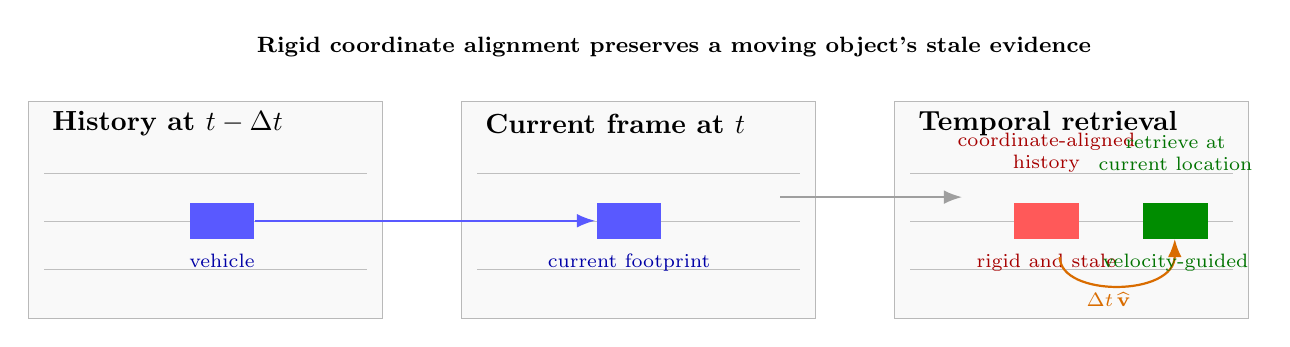
\begin{tikzpicture}[font=\scriptsize, >=Latex, line width=.45pt]
    \node[font=\footnotesize\bfseries] at (8.2,3.45)
      {Rigid coordinate alignment preserves a moving object's stale evidence};
    \foreach \x/\label in {0/History at $t-\Delta t$,5.5/Current frame at $t$,11.0/Temporal retrieval} {
      \draw[fill=gray!5,draw=gray!55] (\x,0) rectangle ++(4.5,2.75);
      \node[anchor=west,font=\bfseries] at (\x+.18,2.47) {\label};
      \draw[gray!50] (\x+.20,.62) -- (\x+4.30,.62);
      \draw[gray!50] (\x+.20,1.23) -- (\x+4.30,1.23);
      \draw[gray!50] (\x+.20,1.84) -- (\x+4.30,1.84);
    }
    \fill[blue!65] (2.05,1.01) rectangle ++(.82,.45);
    \node[below,text=blue!65!black] at (2.46,.94) {vehicle};
    \draw[->,blue!65,thick] (2.88,1.24) .. controls (4.10,1.24) and (5.15,1.24) .. (7.20,1.24);
    \fill[blue!65] (7.22,1.01) rectangle ++(.82,.45);
    \node[below,text=blue!65!black] at (7.63,.94) {current footprint};
    \draw[->,gray!75,thick] (9.55,1.54) -- (11.86,1.54);
    \fill[red!65] (12.52,1.01) rectangle ++(.82,.45);
    \node[below,text=red!65!black] at (12.93,.94) {rigid and stale};
    \draw[->,orange!85!black,thick] (13.10,.78) .. controls (13.10,.27) and (14.56,.27) .. (14.56,1.01);
    \fill[green!55!black] (14.16,1.01) rectangle ++(.82,.45);
    \node[below,text=green!45!black] at (14.57,.94) {velocity-guided};
    \node[align=center,text=red!65!black] at (12.93,2.10) {coordinate-aligned\\history};
    \node[align=center,text=green!45!black] at (14.57,2.10) {retrieve at\\current location};
    \node[text=orange!85!black,align=center] at (13.72,.24)
      {$\Delta t\,\widehat{\mathbf v}$};
  \end{tikzpicture}}}

\newcommand{\fulloverviewdiagram}{%
  \resizebox{\linewidth}{!}{%
  \begin{tikzpicture}[font=\scriptsize, >=Latex, line width=.45pt,
    block/.style={draw=##1!75!black,fill=##1!8,rounded corners=1pt,
      minimum width=2.35cm,minimum height=1.05cm,align=center}]
    \node[block=gray] (img) at (1.2,2.1) {Current multi-view\\images};
    \node[block=gray] (hist) at (1.2,.30) {Historical voxel\\queue};
    \node[block=blue] (lift) at (4.2,2.1) {Voxel hierarchy\\and provisional occupancy};
    \node[block=blue] (dca) at (7.25,2.1) {DCA\\dynamic image updates};
    \node[block=orange] (vve) at (10.25,2.1) {VVE\\local correspondence};
    \node[block=green] (vdsf) at (13.25,2.1) {VDSF\\motion-compensated read};
    \node[block=gray] (out) at (16.15,2.1) {Semantic occupancy\\and velocity};
    \draw[->] (img) -- (lift);
    \draw[->] (lift) -- node[above] {candidate map} (dca);
    \draw[->] (dca) -- (vve);
    \draw[->] (vve) -- node[above] {velocity} (vdsf);
    \draw[->] (vdsf) -- (out);
    \draw[->,dashed,gray!80] (hist.east) -| node[pos=.28,below] {rigidly aligned history} (vve.south);
    \draw[->,dashed,green!55!black] (vve.south) -- ++(0,-.55) -| (vdsf.south);
    \node[font=\footnotesize\bfseries,anchor=west] at (.0,3.08)
      {RoadOcc uses one dynamic candidate map for attention routing and sparse temporal fusion};
  \end{tikzpicture}}}

\newcommand{\fullvelocitydiagram}{%
  \resizebox{\linewidth}{!}{%
  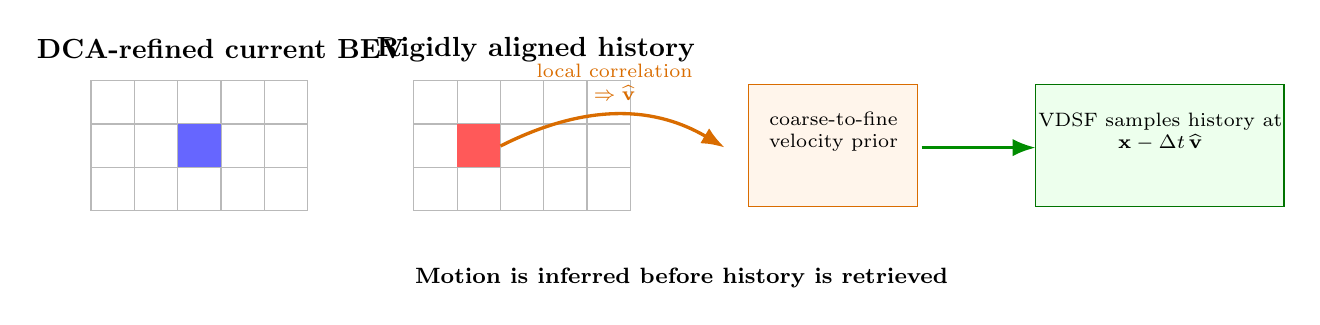
\begin{tikzpicture}[font=\scriptsize, >=Latex, line width=.45pt]
    \node[font=\bfseries] at (1.65,3.45) {DCA-refined current BEV};
    \node[font=\bfseries] at (5.65,3.45) {Rigidly aligned history};
    \foreach \x in {0,...,4} {
      \draw[gray!55] (\x*.55,1.4) rectangle ++(.55,.55);
      \draw[gray!55] (\x*.55,1.95) rectangle ++(.55,.55);
      \draw[gray!55] (\x*.55,2.5) rectangle ++(.55,.55);
      \draw[gray!55] (4.1+\x*.55,1.4) rectangle ++(.55,.55);
      \draw[gray!55] (4.1+\x*.55,1.95) rectangle ++(.55,.55);
      \draw[gray!55] (4.1+\x*.55,2.5) rectangle ++(.55,.55);
    }
    \fill[blue!60] (1.10,1.95) rectangle ++(.55,.55);
    \fill[red!65] (4.65,1.95) rectangle ++(.55,.55);
    \draw[->,orange!85!black,very thick] (5.20,2.22) .. controls (6.35,2.80) and (7.20,2.70) .. (8.05,2.20);
    \node[text=orange!85!black,align=center] at (6.65,3.03)
      {local correlation\\$\Rightarrow\widehat{\mathbf v}$};
    \draw[fill=orange!8,draw=orange!85!black] (8.35,1.45) rectangle ++(2.15,1.55);
    \node[align=center] at (9.43,2.40) {coarse-to-fine\\velocity prior};
    \draw[->,green!55!black,very thick] (10.55,2.20) -- (12.00,2.20);
    \draw[fill=green!7,draw=green!45!black] (12.00,1.45) rectangle ++(3.15,1.55);
    \node[align=center] at (13.58,2.40) {VDSF samples history at\\$\mathbf x-\Delta t\,\widehat{\mathbf v}$};
    \node[font=\footnotesize\bfseries] at (7.5,.55)
      {Motion is inferred before history is retrieved};
  \end{tikzpicture}}}

\newcommand{\fullroutingdiagram}{%
  \resizebox{\linewidth}{!}{%
  \begin{tikzpicture}[font=\scriptsize, >=Latex, line width=.45pt,
    panel/.style={draw=gray!60,fill=gray!5,minimum width=2.85cm,
      minimum height=1.45cm,align=center},
    module/.style={draw=##1!75!black,fill=##1!8,rounded corners=1pt,
      minimum width=3.20cm,minimum height=1.15cm,align=center}]
    \node[font=\footnotesize\bfseries] at (8.0,4.05)
      {The dynamic candidate map is shared, but image updating and temporal retrieval remain distinct};
    \node[panel] (occ) at (1.65,2.15) {Provisional voxel\\semantic state};
    \foreach \x/\y/\fillshade in {0.75/1.55/blue!60,1.12/1.55/blue!60,
      1.49/1.55/orange!85,1.86/1.55/orange!85,2.23/1.55/blue!60,
      1.12/1.92/blue!60,1.49/1.92/orange!85,1.86/1.92/orange!85,
      1.12/2.29/blue!60,1.49/2.29/blue!60,1.86/2.29/orange!85} {
      \fill[\fillshade] (\x,\y) rectangle ++(.31,.31);
    }
    \node[font=\tiny,text=orange!85!black] at (1.65,.92) {dynamic semantic support};
    \node[module=orange] (cand) at (5.55,2.15) {Shared candidate map $\mathbf c_t^s$\\
      dynamic score $\times$ nonempty support};
    \draw[->] (occ) -- (cand);
    \node[panel] (images) at (9.65,3.15) {Current multi-view\\image features};
    \foreach \x in {8.82,9.42,10.02} {
      \draw[gray!60,fill=blue!4] (\x,2.72) rectangle ++(.42,.52);
      \draw[gray!40] (\x+.06,2.83) -- (\x+.36,2.83);
      \draw[gray!40] (\x+.06,2.96) -- (\x+.36,2.96);
    }
    \node[module=blue] (dca) at (13.25,3.15) {DCA\\extra image cross-attention};
    \draw[->,blue!65!black] (cand.north east) |- node[pos=.64,above] {candidate-routed queries} (dca.west);
    \draw[->,blue!65!black] (images) -- (dca);
    \node[panel] (queue) at (9.65,.90) {Aligned history queue};
    \foreach \x/\label in {8.85/$t-2$,9.49/$t-1$,10.13/$t$} {
      \draw[gray!60,fill=green!5] (\x,.53) rectangle ++(.48,.30);
      \node[font=\tiny] at (\x+.24,.34) {\label};
    }
    \node[module=green] (vdsf) at (13.25,.90) {VDSF\\top-$K$ motion-compensated read};
    \draw[->,green!45!black] (cand.south east) |- node[pos=.62,below] {selected dynamic tokens} (vdsf.west);
    \draw[->,green!45!black] (queue) -- node[above] {$\mathbf x-\Delta t\widehat{\mathbf v}$} (vdsf);
    \node[module=gray] (out) at (17.05,2.15) {Updated current\\voxel state};
    \draw[->,blue!65!black] (dca.east) -| (out.north west);
    \draw[->,green!45!black] (vdsf.east) -| (out.south west);
    \node[font=\tiny,text=gray!75,align=center] at (17.05,.63)
      {DCA adds image evidence. VDSF adds only retrieved temporal evidence.};
  \end{tikzpicture}}}

\newcommand{\fullqualdiagram}{%
  \resizebox{\linewidth}{!}{%
  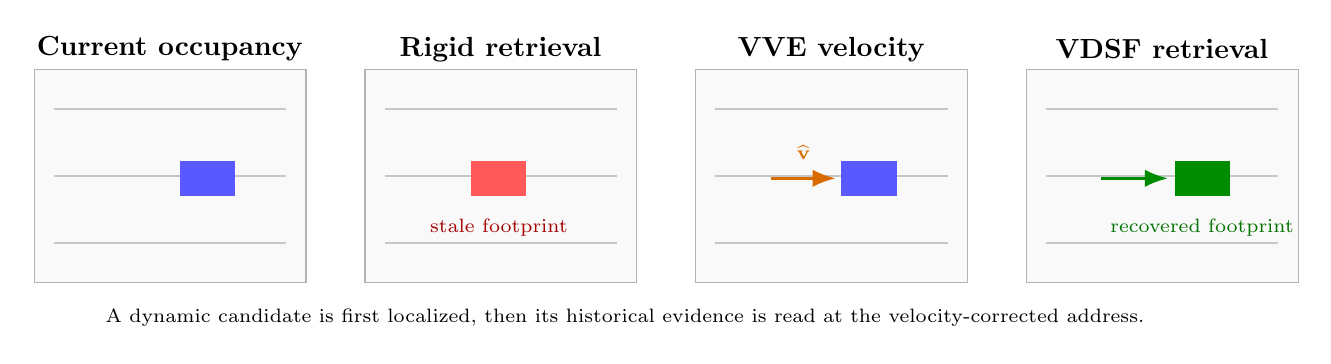
\begin{tikzpicture}[font=\scriptsize, >=Latex, line width=.45pt]
    \foreach \x/\title in {0/Current occupancy,4.2/Rigid retrieval,8.4/VVE velocity,12.6/VDSF retrieval} {
      \draw[fill=gray!5,draw=gray!60] (\x,0) rectangle ++(3.45,2.70);
      \node[font=\bfseries] at (\x+1.72,2.96) {\title};
      \draw[gray!45] (\x+.25,.50) -- (\x+3.20,.50);
      \draw[gray!45] (\x+.25,1.35) -- (\x+3.20,1.35);
      \draw[gray!45] (\x+.25,2.20) -- (\x+3.20,2.20);
    }
    \fill[blue!65] (1.85,1.10) rectangle ++(.70,.44);
    \fill[red!65] (5.55,1.10) rectangle ++(.70,.44);
    \fill[blue!65] (10.25,1.10) rectangle ++(.70,.44);
    \draw[->,orange!85!black,very thick] (9.35,1.32) -- (10.18,1.32);
    \node[text=orange!85!black,above] at (9.77,1.43) {$\widehat{\mathbf v}$};
    \fill[green!55!black] (14.48,1.10) rectangle ++(.70,.44);
    \draw[->,green!55!black,very thick] (13.55,1.32) -- (14.40,1.32);
    \node[text=red!65!black,below] at (5.90,.93) {stale footprint};
    \node[text=green!45!black,below] at (14.83,.93) {recovered footprint};
    \node[align=center] at (7.5,-.45)
      {A dynamic candidate is first localized, then its historical evidence is read at the velocity-corrected address.};
  \end{tikzpicture}}}

\newcommand{\compactretrievaldiagram}{%
  \resizebox{.96\columnwidth}{!}{%
  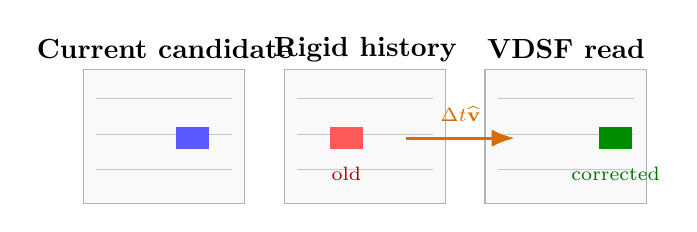
\begin{tikzpicture}[font=\scriptsize, >=Latex, line width=.45pt]
    \foreach \x/\title in {0/Current candidate,2.55/Rigid history,5.10/VDSF read} {
      \draw[fill=gray!5,draw=gray!60] (\x,0) rectangle ++(2.05,1.70);
      \node[font=\bfseries] at (\x+1.03,1.96) {\title};
      \draw[gray!45] (\x+.16,.43) -- (\x+1.89,.43);
      \draw[gray!45] (\x+.16,.88) -- (\x+1.89,.88);
      \draw[gray!45] (\x+.16,1.33) -- (\x+1.89,1.33);
    }
    \fill[blue!65] (1.18,.69) rectangle ++(.42,.28);
    \fill[red!65] (3.13,.69) rectangle ++(.42,.28);
    \fill[green!55!black] (6.55,.69) rectangle ++(.42,.28);
    \draw[->,orange!85!black,very thick] (4.10,.83) -- (5.48,.83);
    \node[text=orange!85!black,above] at (4.79,.92) {$\Delta t\widehat{\mathbf v}$};
    \node[text=red!65!black,below] at (3.34,.59) {old};
    \node[text=green!45!black,below] at (6.76,.59) {corrected};
  \end{tikzpicture}}}

\title{RoadOcc: Learning When to Persist, Transport, or Refresh Memory for Roadside Occupancy Prediction}
\author{Anonymous Authors}

% \iclrfinalcopy
\begin{document}

\maketitle

\begin{abstract}
3D semantic occupancy prediction has advanced rapidly for ego-centric driving,
while camera-only roadside occupancy remains underexplored. Unlike moving ego
sensors, fixed roadside cameras observe a persistent world frame in which static
structure remains aligned but sparse traffic moves. This asymmetry makes history
valuable for weak or occluded actors but dangerous when moving evidence remains
at stale locations. Motion-guided retrieval can relocate historical features,
but the resulting address alone does not indicate whether the retrieved history
is valid for the current voxel. We therefore formulate temporal memory
as semantic-support-supervised routing among evidence sources. For each selected voxel,
\method{} can \emph{persist} with fixed-coordinate history, \emph{transport}
velocity-addressed history, or \emph{refresh} from current evidence when
historical support is unreliable. Dynamic-aware Cross-attention (DCA) localizes
where temporal reasoning is needed, multi-scale voxel velocity estimation (VVE)
combines current and temporal motion cues to determine where history should be
read, and velocity-guided dynamic sparse fusion (VDSF) routes fixed-coordinate,
transported, or current evidence before fusion. Together, they separate source
localization, address construction, and evidence admission. On InfraOcc,
RoadOcc reaches 65.29 mIoU and 32.37 dynamic mIoU, outperforming STCOcc by
4.44 and 4.71 points. Three-seed routing controls, transfer to two temporal
frameworks, and Occ3D-nuScenes results support the design. Code will be released.
\end{abstract}

\section{Introduction}
\label{sec:introduction}

Semantic occupancy prediction reconstructs free space, static layout, and
traffic participants in a common voxel volume. Camera-only methods have made
this representation practical through sparse voxel queries, BEV lifting,
tri-plane features, and unified panoptic volumes
\citep{MonoScene,VoxFormer,OpenOccupancy,Occ3D2023,BEVFormer,TPVFormer,
SurroundOcc,SparseOcc,GaussianFormer}. However, these methods
are predominantly developed for moving platforms, where each observation is
interpreted in an ego-centric frame. A roadside sensor instead repeatedly
observes a persistent scaffold overlaid by sparse, short-lived dynamics. History
is most valuable for weak or occluded actors, yet stale footprints can overwrite
exactly these targets. The fixed world frame therefore shifts the central
temporal problem to local evidence management.
Static history is already aligned, whereas dynamic history must be selectively
relocated or rejected.

The same history can provide either valid support or stale evidence.
Fixed-coordinate memory preserves static layout and can recover weak or occluded vehicle
boundaries, but it does not relocate an object that moved within the fixed
coordinate system. Reading such memory from the former footprint can blur a
dynamic boundary, duplicate an object, or attach it to nearby static layout.
Discarding history avoids these errors but also removes useful support. The
challenge is therefore not simply whether to use history, but to decide where
temporal evidence is needed, where supporting history should be read, and
whether that source remains admissible. These cases can coexist within one scene
or along a single object boundary, making a uniform temporal fusion rule
insufficient.

Recent temporal methods demonstrate the value of multi-frame context for
occupancy, flow, and 3D perception \citep{Cam4DOcc,OccWorld,UniOcc,ALOcc,
STCOcc,LetOccFlow,BEVDet4D,RecurrentBEV,STOccMemory}. Existing designs
already incorporate temporal memory, motion alignment, and adaptive fusion.
These capabilities motivate a source-level view of temporal evidence: motion
specifies a retrieval address, while semantic support informs source selection.
A stationary object may reuse fixed-coordinate memory, a moving object may
retrieve memory near $\mathbf x-\Delta t\,\mathbf v_t(\mathbf x)$, and a newly
appearing object can draw on current evidence. The useful source can vary across
voxels even within one object. We encode these alternatives as three supervised
states, using historical same-class support to train source preferences. This
gives temporal fusion an explicit learning target for selecting among aligned
history, motion-addressed history, and the current observation.
\begin{wrapfigure}{r}{0.65\columnwidth}
  \centering
  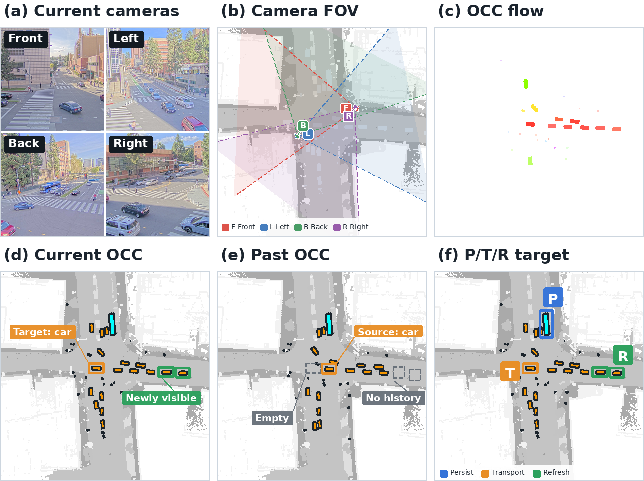
\includegraphics[width=0.65\textwidth]{./Fig0-ptrteaser.pdf}
  \caption{\textbf{Real-scene evidence for explicit source routing.}
  The top row shows current views, camera FOVs, and current-aligned occupancy
  flow (a--c). The bottom row shows current/past occupancy and P/T/R targets
  (d--f), illustrating a
  persistent bus, transported car, and newly visible cars assigned Refresh.}
  \label{fig:motivation}
  \vspace{-10pt}
\end{wrapfigure}
We therefore formulate temporal occupancy as explicit evidence-source routing.
\emph{Should each selected voxel Persist, Transport, or Refresh?} Persist reuses
the fixed-coordinate source, Transport applies backwarp sampling to
velocity-addressed history, and Refresh supplies the current observation.
Flow proposes where history should be read, while semantic-support targets
teach P/T/R preferences over the three sources. Their probabilities condition
fusion, making address construction and source selection separately testable.

RoadOcc realizes this principle through a DCA--VVE--VDSF chain. DCA
localizes the dynamic candidate and refines the current observation. VVE then
combines current and temporal flow into dynamic flow, after which VDSF selects
fixed-coordinate, backwarped, or current evidence. The stages therefore resolve
where temporal reasoning is needed, where history should be read, and which
source should enter fusion. Candidate maps, velocity fields, and route
probabilities provide intermediate representations for studying dynamic
localization, historical addressing, and source selection in the same scene.
Figure~\ref{fig:motivation} grounds the three evidence-source alternatives. 
Our contributions are summarized below.



\begin{itemize}[leftmargin=10pt]
  \item We propose \method{}, which formulates roadside temporal occupancy as
  a Persist--Transport--Refresh routing problem. Semantic-support supervision
  teaches source preferences, connecting motion-based retrieval with learned
  selection of historical and current evidence.
  \item We realize this principle with a staged DCA--VVE--VDSF chain that
  localizes temporal queries, constructs historical addresses, and predicts
  source preferences. DCA localizes dynamic candidates, VVE estimates
  multi-scale dynamic flow, and VDSF performs P/T/R
  source selection before fusion.
  \item We evaluate the source-routing hypothesis with dynamic-first occupancy,
  flow-advected next-frame consistency, and velocity diagnostics.
  Three-seed controls assess source routing, complemented by framework
  transfer, Occ3D-nuScenes evaluation, and temporal-gap generalization.
\end{itemize}

\section{Related Work}
\label{sec:related}

\subsection{Camera Occupancy and Roadside Perception}
Camera occupancy methods lift multi-view image evidence into volumetric
representations. MonoScene \cite{MonoScene} and VoxFormer \cite{VoxFormer} establish image-based semantic scene
completion, while BEVDet, BEVDepth, and BEVFormer improve multi-view lifting and
BEV reasoning \citep{BEVDet,BEVDepth,BEVFormer}. Occupancy-specific designs
span tri-plane, dense,
sparse, Gaussian, and forward--backward representations
\citep{TPVFormer,SurroundOcc,OccFormer,SparseOcc,GaussianFormer,FBOCC}, as well
as panoptic and instance-aware prediction
\citep{PanoOcc,VoxDet}. Unlike MC-BEVRO's roadside BEV occupancy monitoring
\citep{MCBEVRO}, RoadOcc routes evidence for class-aware 3D occupancy.
\begin{wrapfigure}{r}{0.65\columnwidth}
  \vspace{-5pt}
  \centering
  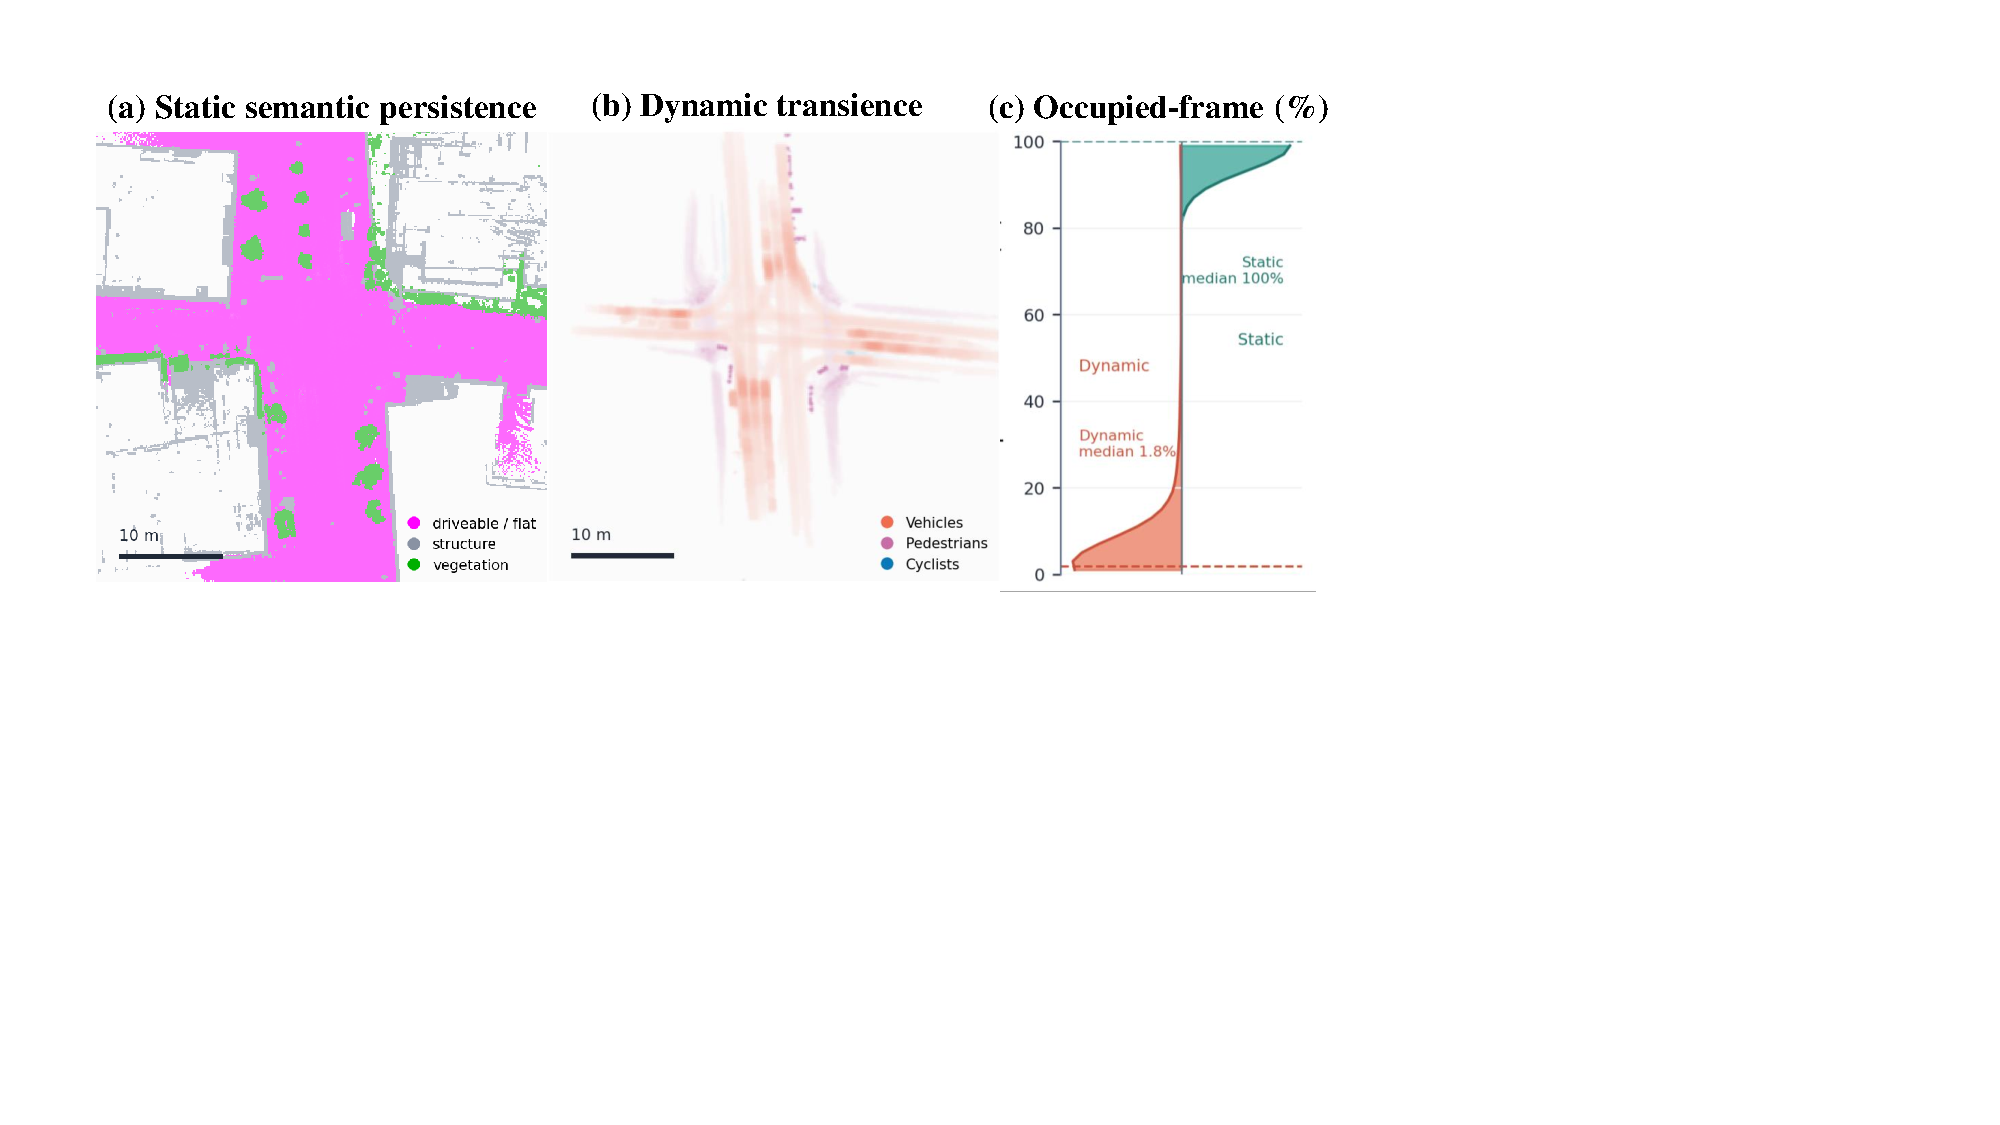
\includegraphics[width=\linewidth]{Fig1-datasetvis.pdf}
  \vspace{-15pt}
  \caption{\textbf{Static-to-dynamic persistence in InfraOcc.}}
  \label{fig:datasetvis}
  % \vspace{-13pt}
\end{wrapfigure}
\vspace{-1pt}
\noindent InfraOcc provides a roadside occupancy benchmark
emphasizing persistent infrastructure \citep{InfraOcc}.
Figure~\ref{fig:datasetvis} reveals its temporal asymmetry. Fixed roadway
structure provides broad, stable support, while dynamic participants form
sparse, short-lived trails. This asymmetry favors retaining static context while
selectively relocating moving evidence.

\subsection{Temporal Occupancy, Motion, and Alignment}

Temporal occupancy methods improve memory through recurrent aggregation,
motion-aware alignment, and explicit association. Recurrent and video-based
models maintain or forecast scene state
\citep{BEVDet4D,RecurrentBEV,SelfOcc,ForecastOcc}, while occupancy--flow methods
couple volumetric semantics with motion
\citep{Cam4DOcc,OccWorld,UniOcc,ALOcc,STCOcc,LetOccFlow,OFMPNet,OmniHDScenes}.
Other approaches organize temporal cues, learn semantic associations, or
retrieve traversal priors \citep{STOccMemory,GDFusion,LinkOcc,LMPOcc}. These
approaches establish complementary tools for temporal retrieval and aggregation.
RoadOcc couples motion-addressed retrieval with semantic-support supervision
over three source states: fixed-coordinate history, transported history, and
current evidence. The predicted state probabilities then condition fusion.

\begin{table*}[htbp]
  \centering
  \begin{minipage}[t]{0.65\textwidth}
    \centering
    \caption{\textbf{Generated GT-flow target at $t+0.5$ s.}
    Zero-flow and GT-flow transport share the inter-frame transform and differ
    only by object displacement. Same/Dyn./Occ. denote unchanged semantics,
    dynamic class, and occupied class. Values are percentages and $N$
    counts valid queries in millions.}
    \label{tab:temporal_verification}
    \footnotesize
    \setlength{\tabcolsep}{0pt}
    \setlength{\belowrulesep}{0pt}
    \setlength{\aboverulesep}{0pt}
    \begin{tabular}{@{}L{2.03cm}C{0.80cm}C{0.85cm}C{0.85cm}C{0.85cm}C{0.85cm}C{0.85cm}C{0.85cm}C{1.08cm}@{}}
      \toprule[1.0pt]
      \multirow{2}{=}{Speed} & \multirow{2}{=}{$N$ (M)} &
      \multicolumn{3}{C{2.55cm}}{Zero-flow transport} &
      \multicolumn{3}{C{2.55cm}}{GT-flow warp} &
      \multirow{2}{=}{$\Delta$ Same} \\
      \cmidrule(lr){3-5}\cmidrule(lr){6-8}
      & & Same & Dyn. & Occ. & Same & Dyn. & Occ. & \\
      \midrule
      All & 11.83 & 72.93 & 78.86 & 90.92 & \textbf{89.21} & \textbf{95.79} & \textbf{99.38} & $+$16.28 \\
      \midrule
      Slow ($<2$ m/s) & 7.87 & 85.19 & 94.08 & 98.80 & 86.51 & \textbf{96.25} & \textbf{99.70} & $+$1.32 \\
      Med. (2--5 m/s) & 1.16 & 71.08 & 71.38 & 87.50 & \textbf{96.65} & \textbf{97.64} & \textbf{99.53} & $+$25.57 \\
      Fast ($\geq5$ m/s) & 2.80 & 39.57 & 39.59 & 70.41 & \textbf{93.73} & \textbf{93.75} & \textbf{98.43} & $+$54.16 \\
      \bottomrule[1.0pt]
    \end{tabular}
  \end{minipage}\hfill
  \begin{minipage}[t]{0.34\textwidth}
    \centering
    \captionof{figure}{\textbf{Motion compensation restores temporal consistency.}
     GT flow preserves dynamic support across speed ranges, whereas fixed-coordinate
     retrieval becomes increasingly misaligned as speed grows.}
     \vspace{-5pt}
    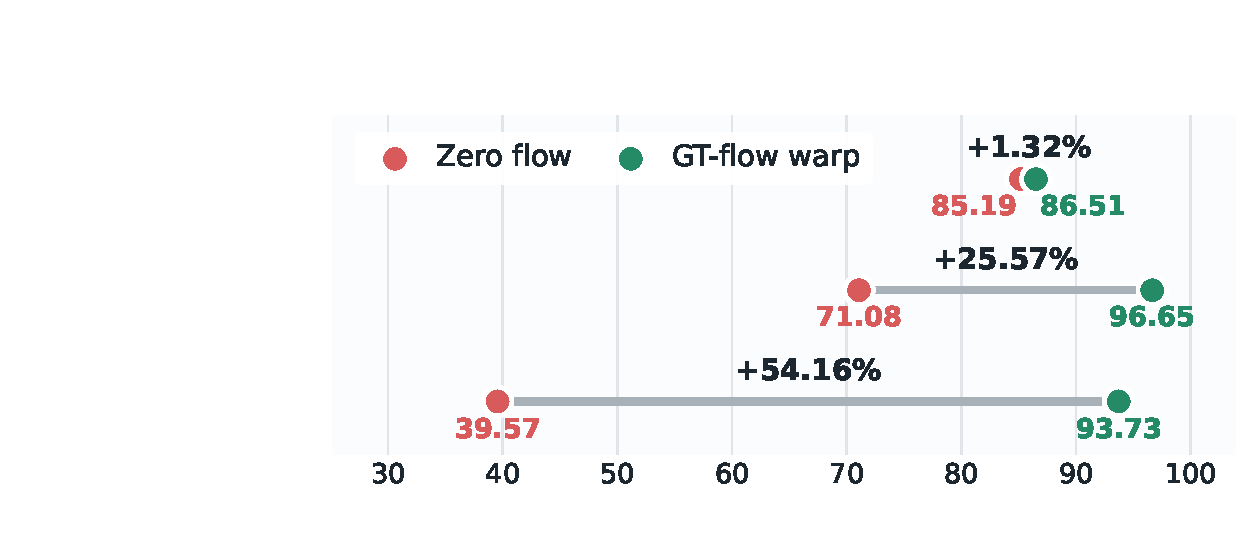
\includegraphics[width=\linewidth]{Fig2-motionissue.pdf}
    \label{fig:speed_temporal_alignment}
  \end{minipage}
\end{table*}
\vspace{-10pt}

Flow-based alignment is closest to this problem. AsyncBEV aligns asynchronous
cross-modal observations with BEV feature flow \citep{AsyncBEV}. In the fixed
roadside setting, Table~\ref{tab:temporal_verification} and
Figure~\ref{fig:speed_temporal_alignment} show that GT-flow warping improves
same-class agreement by 1.32 points for slow objects, but by 25.57 and
54.16 points for medium and fast objects. The rapidly growing gap shows that
fixed-coordinate reuse fails where displacement makes recovery most important, motivating
selective motion compensation.

% Dynamic voxels are sparse and affected by class imbalance and occlusion. Focal
% and class-balanced objectives address related long-tail effects
% \citep{FocalLoss,ClassBalancedLoss}. However, reweighting rare classes does not
% resolve their heterogeneous temporal states because historical evidence may already be
% aligned, displaced, or unsupported. Class imbalance and temporal provenance are
% therefore complementary problems.

\section{Method}
\label{sec:method}

\subsection{Preliminary Analysis}

Let $\mathcal I_t=\{I_t^n\}_{n=1}^{4}$ denote the synchronized roadside images
at time $t$. RoadOcc predicts semantic occupancy $\mathbf y_t$ over a voxel
domain $\Omega$ and a planar velocity field
$\mathbf v_t:\Omega\rightarrow\mathbb R^2$. Among the 18 occupancy states, the
dynamic set is $\mathcal C_{\rm dyn}=\{\text{bicycle, bus, car, motorcycle,
pedestrian, truck}\}$. Velocity is expressed in the common roadside horizontal
frame.

Because fixed roadside cameras share a persistent physical frame, cached
history already lies on the current voxel grid at inference. We only reconcile
relative BEV augmentations during training. Under a locally constant velocity
approximation, history supporting a current voxel
$\mathbf x$ is read from
\begin{equation}
  \widetilde{\mathbf h}_{t-\Delta t}(\mathbf x)=
  \operatorname{Sample}\!\left(\overline{\mathbf h}_{t-\Delta t},
  \mathbf x-\Delta t\,\mathbf v_t(\mathbf x)\right),
  \label{eq:warp}
\end{equation}
where $\overline{\mathbf h}$ is same-grid history and
$\operatorname{Sample}$ is trilinear interpolation. The three candidates are
fixed-coordinate history at $\mathbf x$ (Persist), flow-addressed history at
$\mathbf x-\Delta t\,\mathbf v_t(\mathbf x)$ (Transport), and current evidence
(Refresh). Equation~\ref{eq:warp} specifies only an address. VDSF still decides
whether the sampled source has class-consistent historical support.

\subsection{Overview}
\label{sec:method_overview}

RoadOcc decodes $\{\mathbf V_t^s\}_{s\in\{1/8,1/4,1/2\}}$ from coarse to fine.
As shown in Figure~\ref{fig:overview}, the encoder lifts four camera views into
multi-scale voxel features. At each aggregation stage, DCA determines where
evidence is needed, VVE determines where history should be read, and VDSF
determines which source should enter fusion. The output feature and dynamic flow
seed the next finer stage before occupancy decoding. Supplementary
Figure~\ref{fig:supp_recursive_decoding} visualizes this progression.

\begin{figure*}[t]
  \centering
  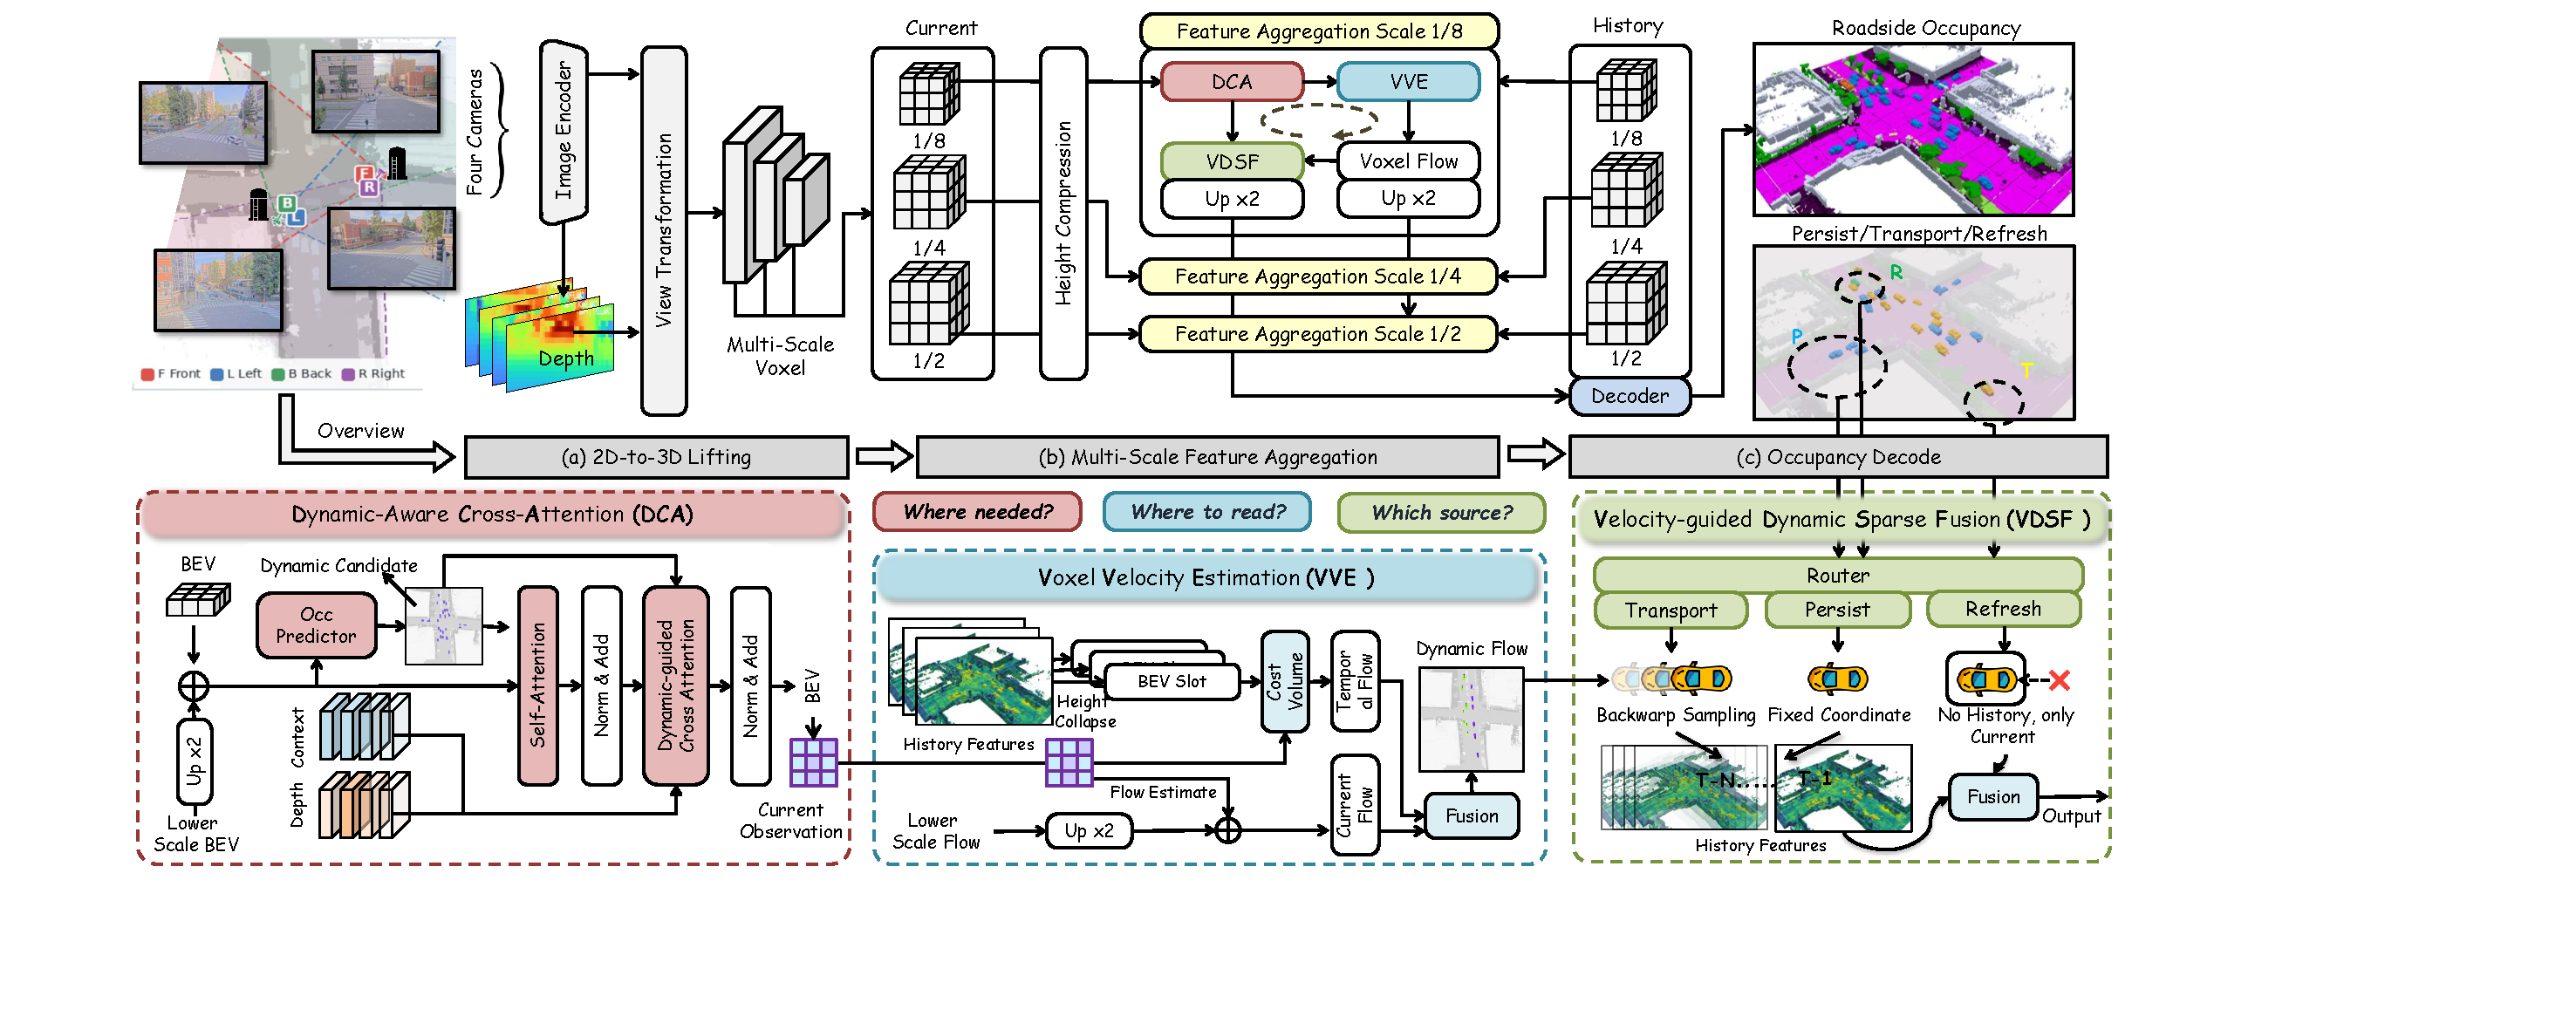
\includegraphics[width=\textwidth]{Fig3-framework.pdf}
  \caption{\textbf{RoadOcc framework.} The image encoder and view
  transformation construct multi-scale voxel features. At each feature
  aggregation scale, DCA produces the current observation, VVE fuses current,
  temporal, and lower-scale flow into dynamic flow, and VDSF routes
  fixed-coordinate, backwarped, or current evidence to fusion. Coarse-to-fine
  outputs feed occupancy decoding for semantic occupancy and voxel flow.}
  \label{fig:overview}
\end{figure*}

\subsection{Dynamic-aware Cross-attention (DCA)}
\label{sec:dca}

Dynamic objects occupy few voxels, so uniformly repeating image cross-attention
spends most computation on stable structure. After the first nonempty-guided
image update, DCA combines the current representation with an upsampled
lower-scale BEV to derive a dynamic candidate. Let
$\boldsymbol\pi_{t,\rm cur}^s$ and $\boldsymbol\pi_{t,\rm sta}^s$ denote the
provisional distributions produced by the current and static prediction heads
after the first image update, and let
$\mathcal C_{\rm sta}^{+}$ contain the static classes and free space. The mean
semantic discrepancy $\delta_{t,\rm sta}^s$ over $\mathcal C_{\rm sta}^{+}$ and
current dynamic probability $p_{t,\rm dyn}^s$ form the candidate map
\begin{equation}
  c_t^s(\mathbf x)
  =\operatorname{Norm}\!\left(\max\!\left\{
  \delta_{t,\rm sta}^s(\mathbf x),p_{t,\rm dyn}^s(\mathbf x)
  \right\}\right).
  \label{eq:dca_candidate}
\end{equation}
Here $\operatorname{Norm}$ divides by the per-sample spatial maximum, clamped to
$10^{-6}$. Discrepancy recovers departures from the static hypothesis, while
dynamic probability retains visible actors. Their maximum also preserves early
semantic misses detected through change evidence.

The candidate map controls a second image cross-attention rather than directly
reweighting the voxel feature. Following projected deformable attention
\citep{BEVFormer} and occupancy-aware reference sampling
\citep{STCOcc}, let $\mathbf q_{t,\mathbf x}^s$ be the BEV query at
$\mathbf x$, $\mathcal R_n(\mathbf x)$ its visible height anchors in camera
$n$, and $\mathbf F_t^n$ the corresponding image feature. DCA retains
$\mathcal R_{n,c}^s(\mathbf x)=\{\mathbf r\in\mathcal R_n(\mathbf x):
u_{\mathbf r}<c_t^s(\mathbf r)\}$ and updates the query as
\begin{equation}
 \begin{aligned}
 \mathbf q_{t,\mathbf x}^{s,+}=\mathbf q_{t,\mathbf x}^{s}
  +\mathbf W_o\frac{1}{|\mathcal V_{\mathbf x}|}
  \sum_{n\in\mathcal V_{\mathbf x}}\sum_{\mathbf r\in
  \mathcal R_{n,c}^s(\mathbf x)}
  \beta_{n,\mathbf r}^s\,
  \mathcal A_{\rm def}\!\left(
  \mathbf q_{t,\mathbf x}^{s},\mathcal P_n(\mathbf r),\mathbf F_t^n\right),
 \end{aligned}
 \label{eq:dca_cross_attention}
\end{equation}
where $\mathbf r=(\mathbf x,z_{\mathbf r})$ indexes a voxel-height score shared
across cameras, $\mathcal V_{\mathbf x}$ contains valid cameras, and
$\mathcal P_n$ projects anchors. Depth consistency $\beta_{n,\mathbf r}^s$
multiplies normalized deformable weights before camera averaging. During
training, $u_{\mathbf r}$ is sampled from a normal distribution
with mean $0.5$ and standard deviation $1$, truncated to $[0,1]$. At inference,
it is fixed to $0.5$. The stochastic
rule exposes uncertain boundary voxels during training, while deterministic
thresholding keeps inference stable. Queries without retained support follow
the residual path unchanged.

The candidate gates a second cross-attention over image depth context and also
allocates VDSF tokens. DCA therefore localizes where additional image and
temporal evidence is needed without repeatedly updating the stable scene.


\subsection{Multi-scale Voxel Velocity Estimation (VVE)}
\label{sec:vve}

DCA refines the current observation but does not locate displaced history. VVE
estimates its address from the DCA feature and nearest valid history. From the
current occupancy distribution $\boldsymbol\pi_t^s(\mathbf x)$, it computes
dynamic support
$d_t^s=\sum_{c\in\mathcal C_{\rm dyn}}\pi_{t,c}^s$ and nonempty support
$e_t^s=1-\pi_{t,\rm free}^s$. Here $d_t^s$ guides height compression into the
current BEV slot $\mathbf B_t^s$, while $e_t^s$ guides temporal token selection.
Applying the same compression to history gives
$\overline{\mathbf B}_{t-\Delta t}^s$.

VVE next compares each current BEV slot with a small neighborhood in the
historical slot, producing the local cost volume
\begin{equation}
  \mathbf K_t^s(\mathbf x,\delta)=
  \left\langle
    \frac{\mathbf B_t^s(\mathbf x)}{\|\mathbf B_t^s(\mathbf x)\|_2},
    \frac{\overline{\mathbf B}_{t-\Delta t}^s(\mathbf x+\delta)}
         {\|\overline{\mathbf B}_{t-\Delta t}^s(\mathbf x+\delta)\|_2}
  \right\rangle,
  \quad \delta\in[-r,r]^2,
  \label{eq:cost_volume}
\end{equation}
where $r=2$ yields a $5\times5$ neighborhood and both norms use an
$\epsilon=10^{-6}$ floor. The cost-volume decoder converts this local
correspondence evidence into temporal flow.

VVE estimates flow recursively rather than solving each resolution in
isolation. Let $s^-$ denote the preceding coarser stage and set the upsampled
lower-scale flow $\mathbf v_{t,\uparrow}^s$ to zero at $1/8$ and to
$\operatorname{Up}_s(\mathbf v_{t,\rm cur}^{s^-})$ otherwise. This prior
initializes the current flow. Current appearance and its semantic embedding
$\mathbf S_t^s$ predict a
current-only correction, while the history feature and cost volume predict the
temporal flow. Their fusion is
\begin{equation}
 \begin{aligned}
  \mathbf v_{t,\rm cur}^s
    &=\mathbf v_{t,\uparrow}^s+\Delta\mathbf v_{t,\rm cur}^s,
  \quad \mathbf v_{t,\rm tmp}^s
    =f_{\rm tmp}(\mathbf B_t^s,\overline{\mathbf B}_{t-\Delta t}^s,
      \mathbf K_t^s),
      \\\widehat{\mathbf v}_t^s
    &=(1-\alpha_t^s)\mathbf v_{t,\rm cur}^s
      +\alpha_t^s\mathbf v_{t,\rm tmp}^s
      +\Delta\mathbf v_{t,\rm ref}^s.
 \end{aligned}
  \label{eq:velocity_prior}
\end{equation}
Here $f_{\rm tmp}$ is the cost-volume decoder and
$\alpha_t^s=0.5\,\mathbf 1_{\rm hist}\max_z d_t^s$ gates history, becoming zero
at sequence starts. The residual $\Delta\mathbf v_{t,\rm ref}^s$ produces the
dynamic flow, which is lifted across height as the VDSF address. Coarse stages
capture motion structure and fine stages refine boundaries.

\subsection{Velocity-guided dynamic sparse fusion (VDSF)}
\label{sec:vdsf}


\paragraph{Velocity-guided sparse fusion.}
Applying the full temporal memory after DCA and VVE would mostly repeat static
context. VDSF makes gather--fuse--scatter \citep{STCOcc} motion aware by
combining DCA guidance with nonempty support under a fixed token budget
\begin{equation}
  \mathbf g_t^s=\operatorname{clip}
  (c_t^s+\eta\,e_t^s,0,1),
  \qquad
  \mathcal X_t^s=\operatorname{TopK}(\mathbf g_t^s),
  \label{eq:vdsf_selection}
\end{equation}
where $\eta$ balances change evidence and occupied support. The selected set
$\mathcal X_t^s$ receives full stage-local history. Its complement uses a short
fixed-coordinate path, preserving background context at lower cost.

Each scale receives multi-frame history features and their VVE motion priors.
For $\mathbf x\in\mathcal X_t^s$, elapsed time converts dynamic flow into a
voxel offset. Backwarp sampling produces the Transport candidate $\mathbf h^T$,
while the fixed-coordinate read produces the Persist candidate $\mathbf h^P$.

\paragraph{Persist--Transport--Refresh routing.}
Dynamic flow supplies the Transport address, and semantic-support supervision
teaches VDSF to select among the three evidence sources.
It retains $\mathbf h^P$ and $\mathbf h^T$ and defines the
current-only Refresh candidate as $\mathbf h^R=\mathbf q_t$. During training,
the route target
is constructed from the current and nearest historical semantic occupancy
labels together with the motion target, and assigns each current dynamic voxel
according to class-consistent historical support:
\begin{equation}
 z_t(\mathbf x)=
 \begin{cases}
 P, & \|\mathbf v_t(\mathbf x)\|\leq\epsilon
      \ \land\ \operatorname{Supp}(\mathbf x),\\
 T, & \|\mathbf v_t(\mathbf x)\|>\epsilon
      \ \land\ \operatorname{Supp}
      (\mathbf x-\Delta t\,\mathbf v_t(\mathbf x)),\\
 R, & \text{otherwise},
 \end{cases}
 \label{eq:ptr_target}
\end{equation}
where $\operatorname{Supp}$ tests same-class occupancy at the same height within
the local correspondence radius. We use $\epsilon=10^{-3}$ m/s and a one-voxel
radius to absorb discretization error. The construction follows the semantic
occupancy label space used by InfraOcc and is evaluated at every execution
scale using its physical cell size, with a native-grid endpoint for
full-resolution supervision. Supported stationary voxels Persist and supported
moving voxels Transport. Refresh supplies the target when the motion-selected
historical candidate lacks support. The motion field in
Eq.~\ref{eq:ptr_target} is the offline supervision target; predicted flow
conditions inference. Supplementary Sec.~\ref{sec:velocity_target_contract}
details target construction.

At each feature aggregation scale, the router combines the current observation,
nearest fixed-coordinate history feature, normalized dynamic flow, and
upsampled coarser P/T/R distribution. It predicts stage-local logits. A
lightweight native head upsamples the finest context with full-resolution flow.
Softmax gives
$\boldsymbol\alpha_t^s=(\alpha_P,\alpha_T,\alpha_R)$ and the routed candidate
\begin{equation}
 \mathbf h^{\rm PTR}_t=\alpha_P\mathbf h^P+
 \alpha_T\mathbf h^T+\alpha_R\mathbf h^R,\qquad
 (\alpha_P,\alpha_T,\alpha_R)=\operatorname{softmax}(\psi(\cdot)).
 \label{eq:ptr_route}
\end{equation}
The three probabilities express a learned preference over evidence sources.
Transport supplies backwarped history, Persist supplies fixed-coordinate
history, and Refresh supplies current evidence. Semantic-support targets
supervise the router; fusion uses its soft probabilities, and argmax identifies
the route shown in diagnostics.

% Defined here to keep the full-width class table close to its discussion in
% Sec.~\ref{sec:main_results}, rather than allowing it to split the objective.
\newcommand{\mainresultstable}{%
\begin{table}[t]
  \caption{\textbf{Main InfraOcc occupancy results.}}
  %RoadOcc (ours) uses
  % strictly current-frame-only input. The two rows marked $^{\mathrm T}$ report
  % their strongest evaluated multi-frame checkpoints. All remaining rows use
  % current-frame-only input.
  \label{tab:infraocc_main_results}
  \centering
  \definecolor{best}{RGB}{255, 180, 180}
  \definecolor{second}{RGB}{255, 230, 180}
  \definecolor{third}{RGB}{255, 255, 200}
  \newlength{\mainmethodwd}
  \newlength{\mainmetricwd}
  \newlength{\mainclasswd}
  \setlength{\mainmethodwd}{0.16\textwidth}
  \setlength{\mainmetricwd}{0.043\textwidth}
  \setlength{\mainclasswd}{\dimexpr(\textwidth-\mainmethodwd-4\mainmetricwd-2\arrayrulewidth)/15\relax}
  \newcommand{\methodcell}[1]{\makebox[\mainmethodwd][l]{##1}}
  \newcommand{\metriccell}[1]{\makebox[\mainmetricwd][c]{##1}}
  \newcommand{\classcell}[1]{\makebox[\mainclasswd][c]{##1}}
  \newcommand{\bestmetriccell}[1]{\cellcolor{best}\metriccell{\textbf{##1}}}
  \newcommand{\secondmetriccell}[1]{\cellcolor{second}\metriccell{\underline{##1}}}
  \newcommand{\thirdmetriccell}[1]{\cellcolor{third}\metriccell{##1}}
  \newcommand{\bestclasscell}[1]{\cellcolor{best}\classcell{\textbf{##1}}}
  \newcommand{\secondclasscell}[1]{\cellcolor{second}\classcell{\underline{##1}}}
  \newcommand{\thirdclasscell}[1]{\cellcolor{third}\classcell{##1}}
  \scriptsize
  \setlength{\tabcolsep}{1.5pt}
  \renewcommand{\arraystretch}{1.05}
  \resizebox{\textwidth}{!}{%
  \begin{tabular}{@{}c|c|*{3}{c}|*{15}{c}@{}}
  \toprule
  \methodcell{Method} & \metriccell{gIoU} & \multicolumn{3}{c|}{\metriccell{mIoU}} & \classcell{\occclassname{Bike}} & \classcell{\occclassname{Bus}} & \classcell{\occclassname{Car}} & \classcell{\occclassname{Motorcycle}} & \classcell{\occclassname{Pedestrian}} & \classcell{\occclassname{Truck}} & \classcell{\occclassname{Other}} & \classcell{\occclassname{Barrier}} & \classcell{\occclassname{Cone}} & \classcell{\occclassname{Driveable}} & \classcell{\occclassname{Sidewalk}} & \classcell{\occclassname{Terrain}} & \classcell{\occclassname{Manmade}} & \classcell{\occclassname{Vegetation}} & \classcell{\occclassname{Free}} \\
  \cmidrule(lr){3-5}
  \methodcell{} & \metriccell{} & \metriccell{all} & \metriccell{dyn} & \metriccell{sta} & \classcell{\classswatch{occBike}} & \classcell{\classswatch{occBus}} & \classcell{\classswatch{occCar}} & \classcell{\classswatch{occMotor}} & \classcell{\classswatch{occPed}} & \classcell{\classswatch{occTruck}} & \classcell{\classswatch{occOther}} & \classcell{\classswatch{occBarrier}} & \classcell{\classswatch{occCone}} & \classcell{\classswatch{occDrive}} & \classcell{\classswatch{occSide}} & \classcell{\classswatch{occTerrain}} & \classcell{\classswatch{occManmade}} & \classcell{\classswatch{occVegetation}} & \classcell{\classswatch{occFree}} \\
  \midrule
  % \rowcolor{gray!5}{\methodcell{Multi-modal (C+L)}} \\
  % \methodcell{BEVFusion~'23} & \metriccell{\secondcell{77.01}} & \metriccell{\secondcell{55.44}} & \metriccell{\secondcell{32.57}} & \metriccell{\secondcell{72.60}} & \classcell{\secondcell{11.03}} & \classcell{\secondcell{65.04}} & \classcell{\secondcell{55.73}} & \classcell{\secondcell{15.26}} & \classcell{\secondcell{29.48}} & \classcell{\bestcell{18.88}} & \classcell{\secondcell{55.04}} & \classcell{\secondcell{72.04}} & \classcell{\secondcell{72.07}} & \classcell{\secondcell{75.43}} & \classcell{\secondcell{73.53}} & \classcell{\secondcell{81.26}} & \classcell{\secondcell{76.82}} & \classcell{\secondcell{74.60}} & \classcell{\secondcell{96.58}} \\
  % \rowcolor{gray!5}\methodcell{ProSD-Occ~'26} & \metriccell{\bestcell{91.78}} & \metriccell{\bestcell{65.87}} & \metriccell{\bestcell{37.92}} & \metriccell{\bestcell{86.82}} & \classcell{\bestcell{30.07}} & \classcell{\bestcell{66.95}} & \classcell{\bestcell{58.55}} & \classcell{\bestcell{19.82}} & \classcell{\bestcell{34.65}} & \classcell{\secondcell{17.51}} & \classcell{\bestcell{72.31}} & \classcell{\bestcell{73.79}} & \classcell{\bestcell{89.68}} & \classcell{\bestcell{94.25}} & \classcell{\bestcell{88.35}} & \classcell{\bestcell{94.73}} & \classcell{\bestcell{90.37}} & \classcell{\bestcell{91.12}} & \classcell{\bestcell{99.09}} \\
  % \midrule
  % \rowcolor{gray!5}{\methodcell{LiDAR-Only (L)}} \\
  % \methodcell{VoxelNet~'18} & \metriccell{\secondcell{75.69}} & \metriccell{\secondcell{53.87}} & \metriccell{31.13} & \metriccell{\secondcell{70.92}} & \classcell{11.08} & \classcell{\bestcell{65.63}} & \classcell{\secondcell{54.52}} & \classcell{\secondcell{13.43}} & \classcell{27.85} & \classcell{14.29} & \classcell{\secondcell{53.39}} & \classcell{72.22} & \classcell{\secondcell{68.26}} & \classcell{\secondcell{75.13}} & \classcell{\secondcell{72.35}} & \classcell{\secondcell{78.99}} & \classcell{\secondcell{74.69}} & \classcell{\secondcell{72.36}} & \classcell{\secondcell{96.31}} \\
  % \methodcell{PointPillars~'19} & \metriccell{70.53} & \metriccell{50.51} & \metriccell{\secondcell{31.55}} & \metriccell{64.74} & \classcell{\bestcell{14.99}} & \classcell{61.62} & \classcell{54.03} & \classcell{11.50} & \classcell{\secondcell{32.62}} & \classcell{\secondcell{14.55}} & \classcell{44.06} & \classcell{\bestcell{73.83}} & \classcell{57.49} & \classcell{72.11} & \classcell{67.67} & \classcell{70.75} & \classcell{66.42} & \classcell{65.56} & \classcell{95.27} \\
  % \rowcolor{gray!5}\methodcell{ProSD-Occ~'26} & \metriccell{\bestcell{90.86}} & \metriccell{\bestcell{63.66}} & \metriccell{\bestcell{33.87}} & \metriccell{\bestcell{85.99}} & \classcell{\secondcell{11.59}} & \classcell{\secondcell{65.62}} & \classcell{\bestcell{58.29}} & \classcell{\bestcell{15.22}} & \classcell{\bestcell{33.09}} & \classcell{\bestcell{19.42}} & \classcell{\bestcell{68.00}} & \classcell{\secondcell{73.75}} & \classcell{\bestcell{90.18}} & \classcell{\bestcell{94.02}} & \classcell{\bestcell{88.14}} & \classcell{\bestcell{95.16}} & \classcell{\bestcell{88.53}} & \classcell{\bestcell{90.17}} & \classcell{\bestcell{98.99}} \\
  % \midrule
  % \rowcolor{gray!5}{\methodcell{Camera-Only (C)}} \\
  \methodcell{BEVDet~'21} & \metriccell{68.62} & \metriccell{45.14} & \metriccell{21.19} & \metriccell{63.11} & \classcell{9.23} & \classcell{42.75} & \classcell{38.04} & \classcell{9.68} & \classcell{15.01} & \secondclasscell{12.45} & \classcell{42.88} & \classcell{70.36} & \classcell{53.77} & \classcell{72.04} & \classcell{68.07} & \classcell{73.09} & \classcell{64.28} & \classcell{60.38} & \classcell{94.87} \\
  \methodcell{BEVFormer~'22} & \metriccell{81.72} & \metriccell{47.76} & \metriccell{10.73} & \metriccell{75.53} & \classcell{7.97} & \classcell{20.39} & \classcell{17.65} & \classcell{3.47} & \classcell{8.62} & \classcell{6.30} & \classcell{42.47} & \thirdclasscell{76.26} & \classcell{72.83} & \classcell{85.19} & \classcell{81.95} & \classcell{88.95} & \classcell{79.52} & \classcell{77.05} & \classcell{97.56} \\
  \methodcell{BEVDepth~'23} & \metriccell{71.89} & \metriccell{46.81} & \metriccell{19.64} & \metriccell{67.19} & \classcell{14.84} & \classcell{33.87} & \classcell{38.74} & \classcell{3.42} & \classcell{16.86} & \classcell{10.14} & \classcell{48.73} & \classcell{71.05} & \classcell{62.37} & \classcell{73.31} & \classcell{69.32} & \classcell{76.07} & \classcell{70.51} & \classcell{66.15} & \classcell{95.54} \\
  \methodcell{TPVFormer~'23} & \metriccell{73.80} & \metriccell{43.09} & \metriccell{4.36} & \metriccell{72.13} & \classcell{0.10} & \classcell{3.69} & \classcell{13.80} & \classcell{0.41} & \classcell{6.86} & \classcell{1.33} & \classcell{42.86} & \classcell{75.29} & \classcell{69.69} & \classcell{80.61} & \classcell{77.62} & \classcell{86.63} & \classcell{72.61} & \classcell{71.70} & \classcell{96.12} \\
  \methodcell{SurroundOcc~'23} & \metriccell{83.78} & \metriccell{50.77} & \metriccell{11.37} & \metriccell{80.32} & \classcell{12.66} & \classcell{21.90} & \classcell{18.54} & \classcell{2.06} & \classcell{9.50} & \classcell{3.55} & \classcell{65.09} & \bestclasscell{79.04} & \classcell{72.70} & \classcell{86.38} & \classcell{83.99} & \classcell{91.10} & \classcell{83.16} & \classcell{81.09} & \classcell{97.80} \\
  \methodcell{CONet~'23} & \metriccell{78.56} & \metriccell{49.25} & \metriccell{18.93} & \metriccell{72.00} & \classcell{3.06} & \classcell{37.24} & \classcell{39.47} & \classcell{4.42} & \classcell{17.64} & \classcell{11.72} & \classcell{45.01} & \classcell{75.31} & \classcell{64.94} & \classcell{84.29} & \classcell{79.45} & \classcell{84.27} & \classcell{72.96} & \classcell{69.79} & \classcell{97.08} \\
  \methodcell{ALOcc~'25} & \metriccell{75.66} & \metriccell{43.31} & \metriccell{5.86} & \metriccell{71.40} & \classcell{8.41} & \classcell{4.04} & \classcell{8.52} & \classcell{0.00} & \classcell{4.48} & \classcell{9.71} & \classcell{63.90} & \classcell{68.97} & \classcell{63.40} & \classcell{90.09} & \classcell{77.77} & \classcell{78.16} & \classcell{65.07} & \classcell{63.85} & \classcell{97.12} \\
  \methodcell{Let Occ Flow~'24} & \metriccell{87.18} & \metriccell{51.38} & \metriccell{8.78} & \thirdmetriccell{83.34} & \classcell{11.27} & \classcell{11.53} & \classcell{14.07} & \classcell{4.34} & \classcell{8.12} & \classcell{3.34} & \classcell{62.06} & \classcell{75.06} & \secondclasscell{85.56} & \classcell{92.55} & \thirdclasscell{85.63} & \thirdclasscell{92.98} & \thirdclasscell{87.10} & \thirdclasscell{85.74} & \classcell{98.56} \\
  \methodcell{SparseOcc~'24} & \metriccell{71.61} & \metriccell{45.42} & \metriccell{9.41} & \metriccell{72.42} & \classcell{1.50} & \classcell{20.94} & \classcell{24.87} & \classcell{0.00} & \classcell{4.60} & \classcell{4.57} & \thirdclasscell{67.68} & \secondclasscell{76.37} & \classcell{61.51} & \classcell{74.67} & \classcell{76.59} & \classcell{88.54} & \classcell{68.79} & \classcell{65.19} & \classcell{96.31} \\
  \methodcell{GaussianFormer~'24} & \metriccell{77.89} & \metriccell{43.63} & \metriccell{10.45} & \metriccell{68.51} & \classcell{3.13} & \classcell{22.11} & \classcell{23.17} & \classcell{1.29} & \classcell{8.21} & \classcell{4.80} & \classcell{36.70} & \classcell{68.54} & \classcell{55.60} & \classcell{82.59} & \classcell{79.37} & \classcell{74.20} & \classcell{77.85} & \classcell{73.21} & \classcell{96.71} \\
  \methodcell{CRT-Fusion-S~'24} & \thirdmetriccell{88.73} & \thirdmetriccell{55.94} & \metriccell{21.98} & \metriccell{81.40} & \classcell{13.02} & \classcell{45.16} & \classcell{38.48} & \classcell{7.34} & \classcell{18.99} & \classcell{8.90} & \classcell{63.53} & \classcell{71.99} & \classcell{74.82} & \thirdclasscell{93.38} & \classcell{84.40} & \classcell{91.19} & \classcell{86.39} & \classcell{85.53} & \thirdclasscell{98.73} \\
  \methodcell{STCOcc-S~'25} & \metriccell{78.54} & \metriccell{50.71} & \metriccell{23.48} & \metriccell{71.14} & \classcell{13.43} & \thirdclasscell{47.83} & \thirdclasscell{39.62} & \classcell{10.21} & \classcell{17.83} & \classcell{11.93} & \classcell{50.18} & \classcell{71.54} & \classcell{58.33} & \classcell{90.30} & \classcell{78.78} & \classcell{84.90} & \classcell{67.72} & \classcell{67.32} & \classcell{97.47} \\
  \methodcell{CRT-Fusion~'24} & \metriccell{80.35} & \metriccell{53.83} & \thirdmetriccell{27.02} & \metriccell{73.94} & \secondclasscell{32.58} & \classcell{46.63} & \classcell{39.49} & \secondclasscell{12.22} & \thirdclasscell{20.81} & \classcell{10.41} & \classcell{53.08} & \classcell{72.27} & \classcell{68.15} & \classcell{89.06} & \classcell{79.09} & \classcell{84.48} & \classcell{72.06} & \classcell{73.30} & \classcell{97.68} \\
  \methodcell{STCOcc~'25} & \secondmetriccell{92.54} & \secondmetriccell{60.85} & \secondmetriccell{27.66} & \secondmetriccell{85.74} & \thirdclasscell{27.13} & \secondclasscell{48.78} & \secondclasscell{44.93} & \thirdclasscell{10.23} & \bestclasscell{22.85} & \thirdclasscell{12.03} & \secondclasscell{68.84} & \classcell{70.93} & \thirdclasscell{81.60} & \secondclasscell{95.88} & \secondclasscell{89.41} & \secondclasscell{95.36} & \secondclasscell{91.85} & \secondclasscell{92.04} & \secondclasscell{99.18} \\
  \methodcell{\textbf{RoadOcc (ours)}} & \bestmetriccell{94.03} & \bestmetriccell{65.29} & \bestmetriccell{32.37} & \bestmetriccell{89.98} & \bestclasscell{37.60} & \bestclasscell{55.46} & \bestclasscell{49.36} & \bestclasscell{13.01} & \secondclasscell{22.66} & \bestclasscell{16.13} & \bestclasscell{87.66} & \classcell{72.05} & \bestclasscell{86.03} & \bestclasscell{97.85} & \bestclasscell{92.81} & \bestclasscell{96.90} & \bestclasscell{92.91} & \bestclasscell{93.66} & \bestclasscell{99.35} \\
  \bottomrule
  \end{tabular}%
  }
  \end{table}%
}
\mainresultstable
Let $\mathbf H_t^{\rm PTR,s}(\mathbf x)$ concatenate the routed multi-frame
history at scale $s$. VDSF combines this temporal evidence with
the current observation and its semantic embedding through the fusion MLP
\begin{equation}
 \mathbf q_{t,\rm fuse}^s(\mathbf x)=\mathbf q_t^s(\mathbf x)+
 \Phi_s\!\left([\mathbf q_t^s(\mathbf x),
 \mathbf H_t^{\rm PTR,s}(\mathbf x),
 \operatorname{Emb}(\boldsymbol\pi_t^s(\mathbf x))]\right).
 \label{eq:vdsf_fusion}
\end{equation}
The output residual is scattered to $\mathcal X_t^s$ and joined with the
background path. The fused volume and dynamic flow feed the next scale and are
retained for subsequent frames. Detailed memory, token, source-matching, and
routing settings appear in supplementary Secs.~\ref{sec:exact_contract}
and~\ref{sec:controlled}.


\subsection{Training Objective}
\label{sec:objective}

Training jointly optimizes four functional objectives.
\begin{equation}
  \mathcal L=\lambda_{\rm depth}\mathcal L_{\rm depth}+
  \mathcal L_{\rm sem}+
  \lambda_{\rm mot}\mathcal L_{\rm mot}+
  \lambda_{\rm route}\mathcal L_{\rm route}.
  \label{eq:loss}
\end{equation}
$\mathcal L_{\rm depth}$ supervises camera depth for view transformation, while
$\mathcal L_{\rm sem}$ covers full- and multi-scale occupancy together with the
static, dynamic, and DCA auxiliaries. $\mathcal L_{\rm mot}$ supervises
the dynamic flow used for backwarp sampling, whereas $\mathcal L_{\rm route}$
supervises the P/T/R router on valid dynamic voxels. Together, they separate
where history features are read from which source enters fusion. Full target
construction, weights, and schedules are given in supplementary
Sec.~\ref{sec:training_objectives}.

% \begin{figure}[t]
%   \centering
%   
\includegraphics[width=\columnwidth]{\figdir/roadocc_sparse_selection.png}
%   \caption{\textbf{Flow-guided dynamic sparse fusion at the finest decoder
%   stage.} The visualizer reports the guidance score, selected top-$K$ mask,
%   dynamic ground truth, and semantic occupancy. VDSF reads history only at
%   selected tokens, while the flow field determines the source address of each
%   read.}
%   \label{fig:dynamic_retrieval}
% \end{figure}


\begin{figure*}[t]
  \centering
  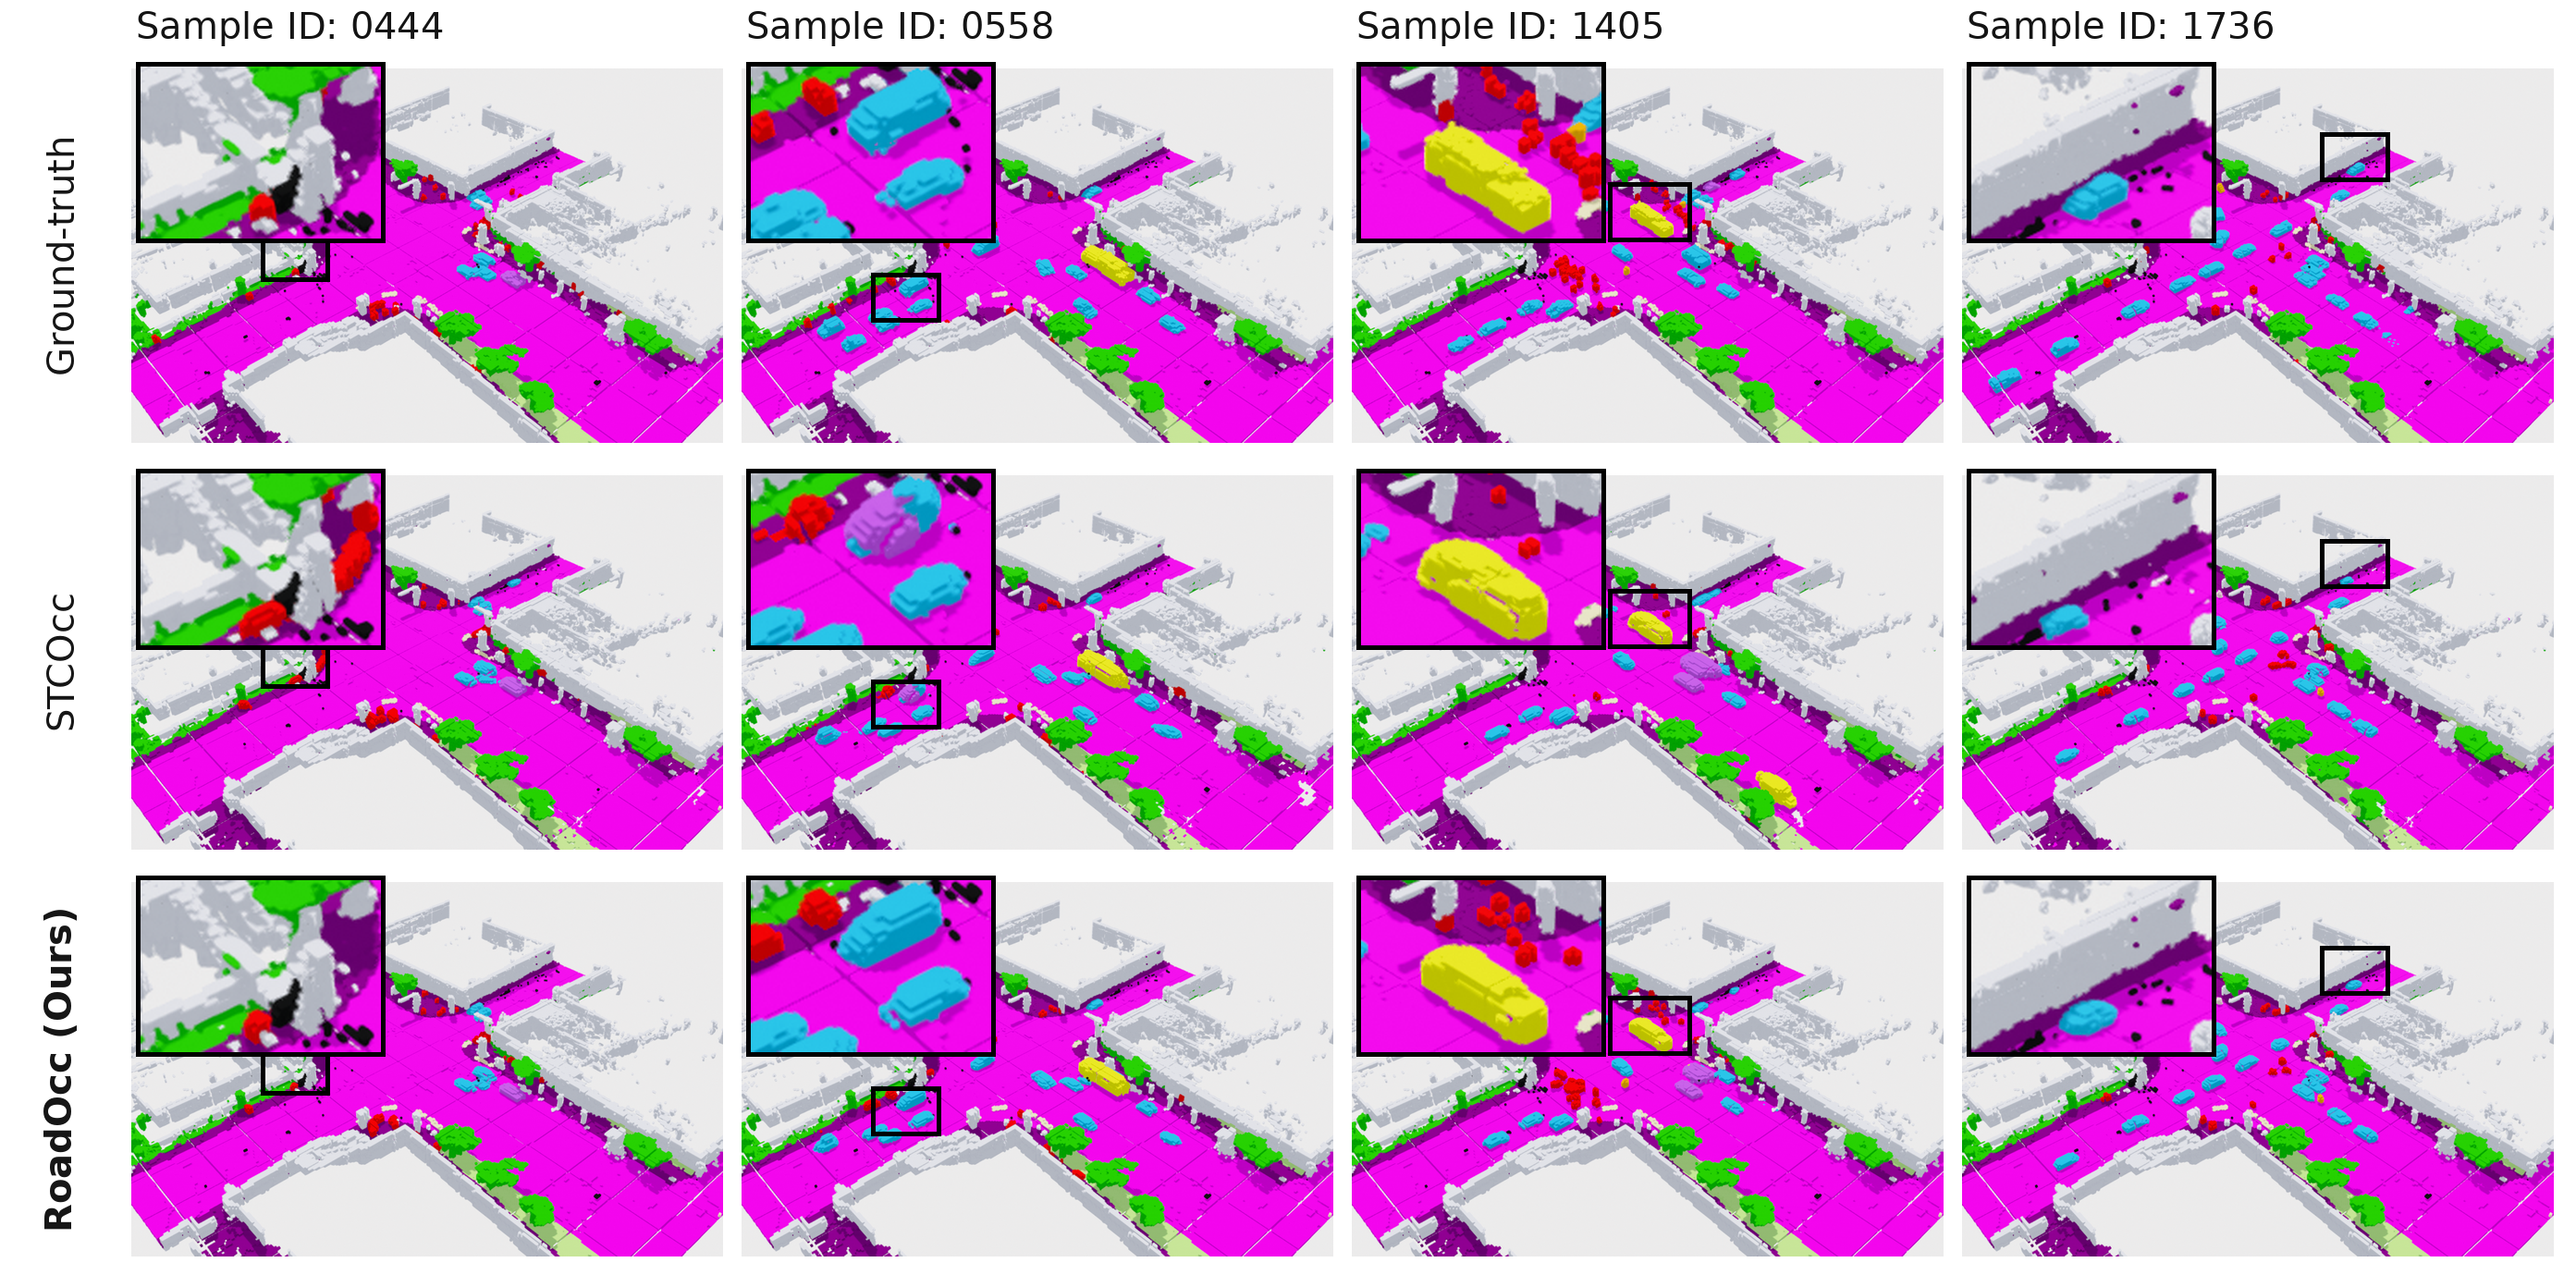
\includegraphics[width=\textwidth]{Fig4-comparison.png}
  \caption{\textbf{Qualitative comparison with STCOcc.}
  RoadOcc more closely recovers dynamic-object presence, semantic identity,
  and geometry, including spurious pedestrian occupancy, vehicle-class
  confusion, bus-shape distortion, and an incomplete car footprint.}
  \label{fig:qualitative_comparison}
\end{figure*}
\begin{table*}[!t]
  \centering
  \caption{\textbf{Joint occupancy--velocity comparison.}}
  \label{tab:joint_results}
  \footnotesize
  \definecolor{ptrrow}{RGB}{239,247,252}
  \setlength{\tabcolsep}{1pt}
  \setlength{\belowrulesep}{0pt}
  \setlength{\aboverulesep}{0pt}
  \begin{tabular}{@{}L{3.55cm}|C{0.95cm}C{0.95cm}C{0.95cm}C{0.95cm}C{0.95cm}|C{1.90cm}|C{1.30cm}C{1.00cm}@{}}
    \toprule
    \multicolumn{1}{C{4.11cm}|}{\multirow{2}{=}{Method}} &
    \multicolumn{5}{c|}{Occupancy} & \multicolumn{1}{c|}{Velocity} &
    \multicolumn{2}{c}{Diagnostics} \\
    \cmidrule(lr){2-6}\cmidrule(lr){7-7}\cmidrule(l){8-9}
    & mIoU & Dyn. & Sta. & gIoU & RayIoU & \mbox{Direct MAVE} & \mbox{\scriptsize TP-MAVE} & DSR \\
    \midrule
    CRT-Fusion~(NeurIPS 2024) & 53.83 & 27.02 & 73.94 & 80.35 & 48.08 & 2.227 & 1.839 & 57.56 \\
    \quad + VDSF P/T/R & 57.15 & 28.30 & 78.79 & 83.46 & 52.34 & 1.990 & 1.958 & \underline{59.45} \\
    \rowcolor{ptrrow}\quad $\Delta$ & $+$3.32 & $+$1.28 & $+$4.85 & $+$3.11 & $+$4.26 & $-$0.237 & $+$0.119 & $+$1.89 \\
    STCOcc~(CVPR 2025) & 60.85 & 27.66 & 85.74 & 92.54 & 55.94 & 1.946 & 0.703 & 57.12 \\
    \quad + VDSF P/T/R & \underline{61.81} & \underline{28.80} & \underline{86.56} & \underline{93.59} & \underline{58.07} & \underline{1.770} & \textbf{0.648} & 58.78 \\
    \rowcolor{ptrrow}\quad $\Delta$ & $+$0.96 & $+$1.14 & $+$0.82 & $+$1.05 & $+$2.13 & $-$0.176 & $-$0.055 & $+$1.66 \\
    \midrule
    \textbf{RoadOcc (ours)} & \textbf{65.29} & \textbf{32.37} & \textbf{89.98} & \textbf{94.03} & \textbf{65.44} & \textbf{1.669} & \underline{0.661} & \textbf{61.11} \\
    \bottomrule
  \end{tabular}
\end{table*}


\section{Experiments}
\label{sec:experiments}

% \subsection{Setup}
% \label{sec:setup}

\noindent\textbf{Dataset and metrics.}
We evaluate camera-only roadside occupancy on InfraOcc, derived from V2X-Real
\citep{V2XReal,InfraOcc}. Four synchronized views are mapped to 18 occupancy
states. Under the InfraOcc protocol, semantic mIoU excludes construction
vehicle, trailer, other flat, and Free. Free IoU is reported separately in the
class-wise table. We report semantic and geometric IoU, next-frame dynamic IoU,
and motion coverage. Direct MAVE covers all GT dynamic voxels, while TP-MAVE
conditions on semantic matches and is paired with recall (DSR).
InfraOcc provides the dense fixed-roadside camera-only protocol used throughout.
Since existing roadside datasets mainly provide object-level labels, we
complement the benchmark results with matched backbone transfer and controlled
studies. Full benchmark details appear in the supplement.

\noindent\textbf{Implementation details.}
RoadOcc uses a ResNet-50 backbone, $256\times704$ images, and three voxel stages
from 0.8 m to 0.4 m over $[-64,64]\times[-64,64]\times[-4.8,1.6]$ m. Frames are
0.5 s apart. AdamW training runs for 24 epochs from $5\times10^{-4}$ with
$10^{-2}$ weight decay and cosine annealing. Comparisons share the voxel range,
ignored classes, and evaluator. Controlled variants keep the
backbone, data split, optimizer, schedule and other
configuration fixed.

% The $-$S suffix disables temporal history while
% retaining the task architecture and training protocol, whereas unmarked temporal
% variants use their corresponding memory path. 

\subsection{Main Results}
\label{sec:main_results}


% We first establish the official occupancy gain in
% Table~\ref{tab:infraocc_main_results}, then test whether this gain is accompanied
% by improved motion accuracy and historical-support coverage in
% Table~\ref{tab:joint_results}.
% Table~\ref{tab:infraocc_main_results} addresses the first using
% current-frame camera baselines. Table~\ref{tab:joint_results} addresses the
% second under a common temporal protocol with occupancy, velocity, and support
% diagnostics.

\noindent\textbf{InfraOcc occupancy benchmark.}
Table~\ref{tab:infraocc_main_results} tests whether the proposed routing chain
improves occupancy under the InfraOcc evaluator. RoadOcc establishes a new state
of the art at 65.29 mIoU, a $+$4.44 gain over STCOcc. Dynamic mIoU rises by
$+$4.71 to 32.37, while static mIoU rises by $+$4.24 to 89.98. The joint gain
follows the framework's staged decisions. DCA supplies the dynamic candidate,
VVE converts current and temporal flow into source addresses, and the VDSF
router selects among fixed-coordinate, backwarped, and current evidence.
Together, they improve transient-object recovery without destabilizing the
persistent roadside scaffold.

\noindent\textbf{Joint occupancy--velocity behavior.}
Table~\ref{tab:joint_results} tests whether these occupancy gains follow the
proposed routing mechanism. Direct MAVE measures the quality of the VVE address,
while DSR measures the dynamic support recovered by the complete routing path.
Relative to STCOcc, RoadOcc lowers Direct MAVE from 1.946 to 1.669 and raises
DSR from 57.12 to 61.11. This paired improvement supports both routing
decisions. VVE
improves the dynamic flow used for backwarp sampling, while P/T/R determines
which source is admissible for fusion.
Adding VDSF P/T/R to CRT-Fusion and STCOcc likewise raises Dyn. by $+$1.28 and
$+$1.14, respectively, while improving Direct MAVE and DSR. The consistent
trend across both backbones links the gain to source-aware routing rather than
backbone-specific capacity. TP-MAVE conditions on semantic matches and must be
read with DSR. For CRT-Fusion, the $+$1.89 DSR gain indicates broader dynamic
recovery even though the conditional error over matched voxels increases.

\noindent\textbf{Qualitative occupancy recovery.}
Figure~\ref{fig:qualitative_comparison} supports the aggregate dynamic gain with
representative matched scenes. STCOcc produces
stale or spurious pedestrian occupancy, confuses a vehicle class, distorts a
bus footprint, and incompletely recovers a car. By correcting displaced reads
and rejecting unsupported history, RoadOcc suppresses these errors and recovers
object identity and extent more consistently with GT, while preserving the
surrounding roadway.

\subsection{Ablation Studies}
\label{sec:ablation}

Using \citet{STCOcc} as the baseline, we hold the backbone, token budget, temporal-memory
configuration, and training protocol fixed unless explicitly varied.
Tables~\ref{tab:temporal_design}, \ref{tab:flow_branch}, and
\ref{tab:motion_counterfactual} then isolate component composition,
historical-address correction, and P/T/R source selection, respectively.

\begin{wraptable}[9]{r}{0.50\columnwidth}
  \vspace{-15pt}
  \centering
  \captionof{table}{\textbf{Component ablation.}}
  \label{tab:temporal_design}
  \footnotesize
  \renewcommand{\arraystretch}{1.00}
  \setlength{\tabcolsep}{0pt}
  \setlength{\belowrulesep}{0pt}
  \setlength{\aboverulesep}{0pt}
  \begin{tabular}{@{}C{1.00cm}|C{0.82cm}C{0.82cm}C{0.82cm}C{0.82cm}|C{0.85cm}C{0.85cm}C{0.85cm}@{}}
    \toprule[1.0pt]
    \multicolumn{1}{C{0.95cm}|}{\multirow{2}{=}{Base}} &
    \multicolumn{4}{c|}{Design} &
    \multicolumn{3}{c}{Output $\uparrow$} \\
    \cmidrule(lr){2-5}\cmidrule(l){6-8}
     & DCA & VVE & VDSF & P/T/R & All & Dyn. & Nxt. \\
    \midrule
    \cmark &  &  &  &  & 60.85 & 27.66 & 26.74 \\
    \cmark &  &  & \cmark &  & 61.05 & 28.01 & 26.99 \\
    \cmark & \cmark &  &  &  & 61.69 & 28.55 & 27.64 \\
    \cmark & \cmark &  & \cmark &  & 63.01 & 30.10 & 29.44 \\
    \cmark & \cmark & \cmark & \cmark &  & 64.17 & 30.97 & 30.78 \\
    \cmark & \cmark & \cmark & \cmark & \cmark & \textbf{65.29} & \textbf{32.37} & \textbf{31.72} \\
    \bottomrule[1.0pt]
  \end{tabular}
\end{wraptable}

\begin{figure*}[t]
  \centering
  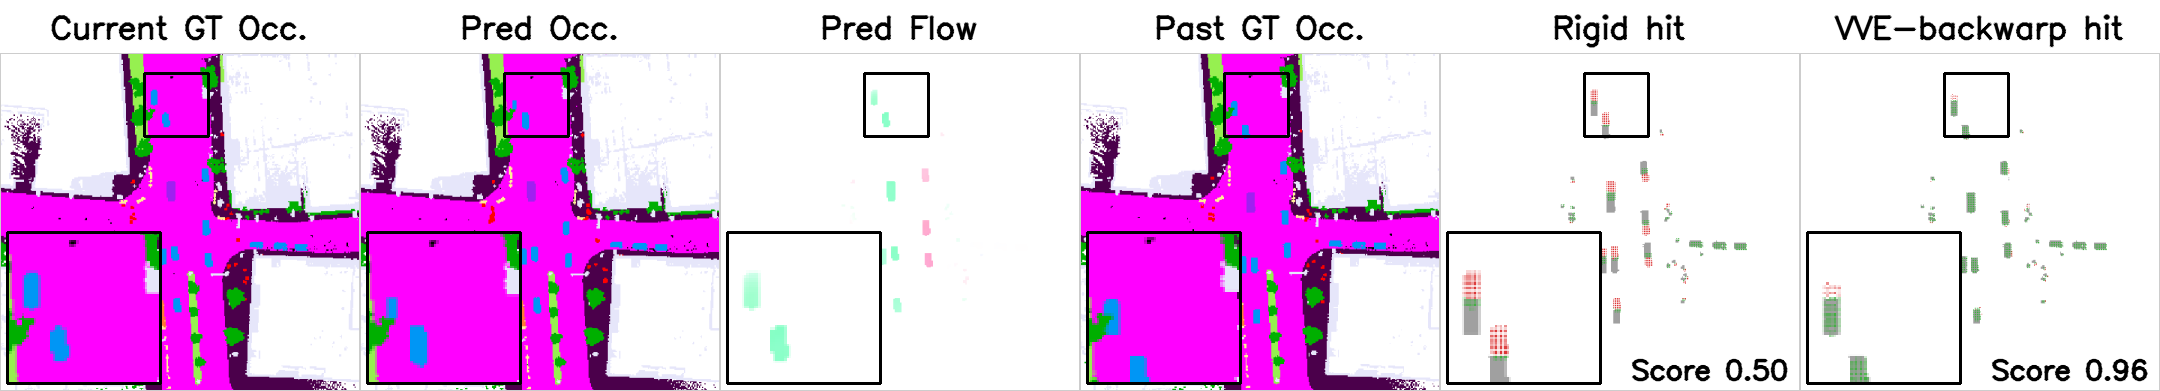
\includegraphics[width=1.0\textwidth]{Fig5-backwarp.png}
  \caption{\textbf{Velocity-guided historical retrieval.} With queried
  dynamic targets fixed by current GT, the panels show the end-to-end occupancy
  prediction and compare a fixed-coordinate read with the VVE backtrace into aligned past
  GT. Black boxes are enlarged in the insets. \hitbox{hitmatch} same-class
  matches, \hitbox{hitmismatch} unmatched targets, and \hitbox{hitother} other
  queried voxels are shown in green, red, and gray, respectively.
  The score is the same-class hit rate within the one-voxel matching radius.}
  \label{fig:vve_backwarp}
\end{figure*}

\noindent\textbf{Overall ablation.}
Table~\ref{tab:temporal_design} follows the routing chain. VDSF alone adds only
0.20 mIoU because moving evidence remains at unresolved source locations. DCA
and VDSF then raise Dyn. by $+$1.55 and Nxt. by $+$1.80, showing that the dynamic
candidate identifies where sparse temporal fusion is useful. With these
locations fixed, VVE adds $+$1.16 mIoU by correcting the dynamic flow and
backwarp-sampling address. P/T/R adds a further $+$1.12 mIoU by selecting
fixed-coordinate, backwarped, or current evidence for fusion. The ordered gains
therefore track the three framework decisions rather than undifferentiated
temporal capacity.

\noindent\textbf{Address correction and source selection.}
With capacity and token budget fixed, the fixed-coordinate and VVE reads in
Table~\ref{tab:flow_branch} differ only in historical address. VVE raises Dyn. by
$+$0.87, lowers dMAVE from 2.146 to 1.690, and raises DSR by $+$1.51, directly
verifying address correction. With that address fixed, P/T/R adds $+$1.40 Dyn.
and $+$1.76 DSR. This second transition shows that a corrected address is useful
only when the fusion stage can select supported evidence.


\begin{wraptable}[16]{r}{0.48\columnwidth}
  \vspace{-5pt}
  \centering
  \captionof{table}{\textbf{Controlled address and source selection.} All
  variants use the same sparse-token budget and model capacity.}
  \label{tab:flow_branch}
  \footnotesize
  \renewcommand{\arraystretch}{1.00}
  \setlength{\tabcolsep}{0.4pt}
  \setlength{\belowrulesep}{0pt}
  \setlength{\aboverulesep}{0pt}
  \begin{tabular}{@{}C{1.50cm}|C{1.00cm}C{1.00cm}|C{0.75cm}C{0.75cm}C{0.75cm}C{0.75cm}@{}}
    \toprule[1.0pt]
    \multicolumn{1}{>{\centering\arraybackslash}m{1.38cm}|}{\multirow{2}{*}{Variant}} &
     \multicolumn{2}{c|}{Design} & \multicolumn{4}{c}{Output} \\
    \cmidrule(lr){2-3}\cmidrule(l){4-7}
    & VVE & P/T/R & Dyn.$\uparrow$ & Nxt.$\uparrow$ & dM$\downarrow$ & DSR$\uparrow$ \\
    \midrule
    \mbox{Fixed read} &  &  & 30.10 & 29.44 & 2.146 & 57.84 \\
    \mbox{VVE read} & \cmark &  & 30.97 & 30.78 & 1.690 & 59.35 \\
    \textbf{Full} & \cmark & \cmark & \textbf{32.37} & \textbf{31.72} & \textbf{1.669} & \textbf{61.11} \\
    \bottomrule[1.0pt]
  \end{tabular}
  \centering

  \captionof{table}{\textbf{P/T/R routing controls.} Mean $\pm$ standard
  deviation over three independent seeds.}
  \label{tab:motion_counterfactual}
  \footnotesize
  \renewcommand{\arraystretch}{1.05}
  \setlength{\tabcolsep}{0.7pt}
  \setlength{\belowrulesep}{0pt}
  \setlength{\aboverulesep}{0pt}
  \begin{tabular}{@{}l|cccc@{}}
    \toprule[1.0pt]
    Variant & Dyn.$\uparrow$ & Nxt.$\uparrow$ & DSR$\uparrow$ & dM$\downarrow$ \\
    \midrule
    None & 30.97$\pm$.27 & 30.78$\pm$.34 & 59.35$\pm$.39 & 1.690$\pm$.019 \\
    Gate & 31.25$\pm$.20 & 30.94$\pm$.30 & 59.75$\pm$.45 & 1.685$\pm$.018 \\
    State & 31.88$\pm$.18 & 31.38$\pm$.25 & 60.52$\pm$.40 & 1.675$\pm$.017 \\
    \textbf{Full} & \textbf{32.37$\pm$.11} & \textbf{31.72$\pm$.26} & \textbf{61.11$\pm$.38} & \textbf{1.669$\pm$.020} \\
    \bottomrule[1.0pt]
  \end{tabular}
\end{wraptable}


\noindent\textbf{P/T/R routing controls.}
Table~\ref{tab:motion_counterfactual} holds DCA--VVE--VDSF fixed and isolates
source selection. Gate tests adaptive weighting, State introduces explicit
P/T/R states, and Full uses the predicted routes in fusion. State exceeds Gate
by $+$0.63 Dyn., $+$0.44 Nxt., and $+$0.77 DSR, while Full adds another
$+$0.49, $+$0.34, and $+$0.59. Overall, Full surpasses Gate by $+$1.12 Dyn.,
$+$0.78 Nxt., and $+$1.36 DSR, attributing the gain to explicit source states
and route-conditioned fusion rather than adaptive weighting alone.

% \noindent\textbf{Dynamic behavior.}
% Recall and footprint diagnostics distinguish missing support from semantic
% confusion, while ghost occupancy measures stale evidence left at a previous
% location. Together with the speed-stratified analysis in
% Table~\ref{tab:temporal_verification}, these diagnostics test whether the model
% improves moving objects without disturbing already aligned slow or stationary
% participants.




\begin{wrapfigure}{r}{0.68\columnwidth}
  \vspace{-7pt}
  \centering
  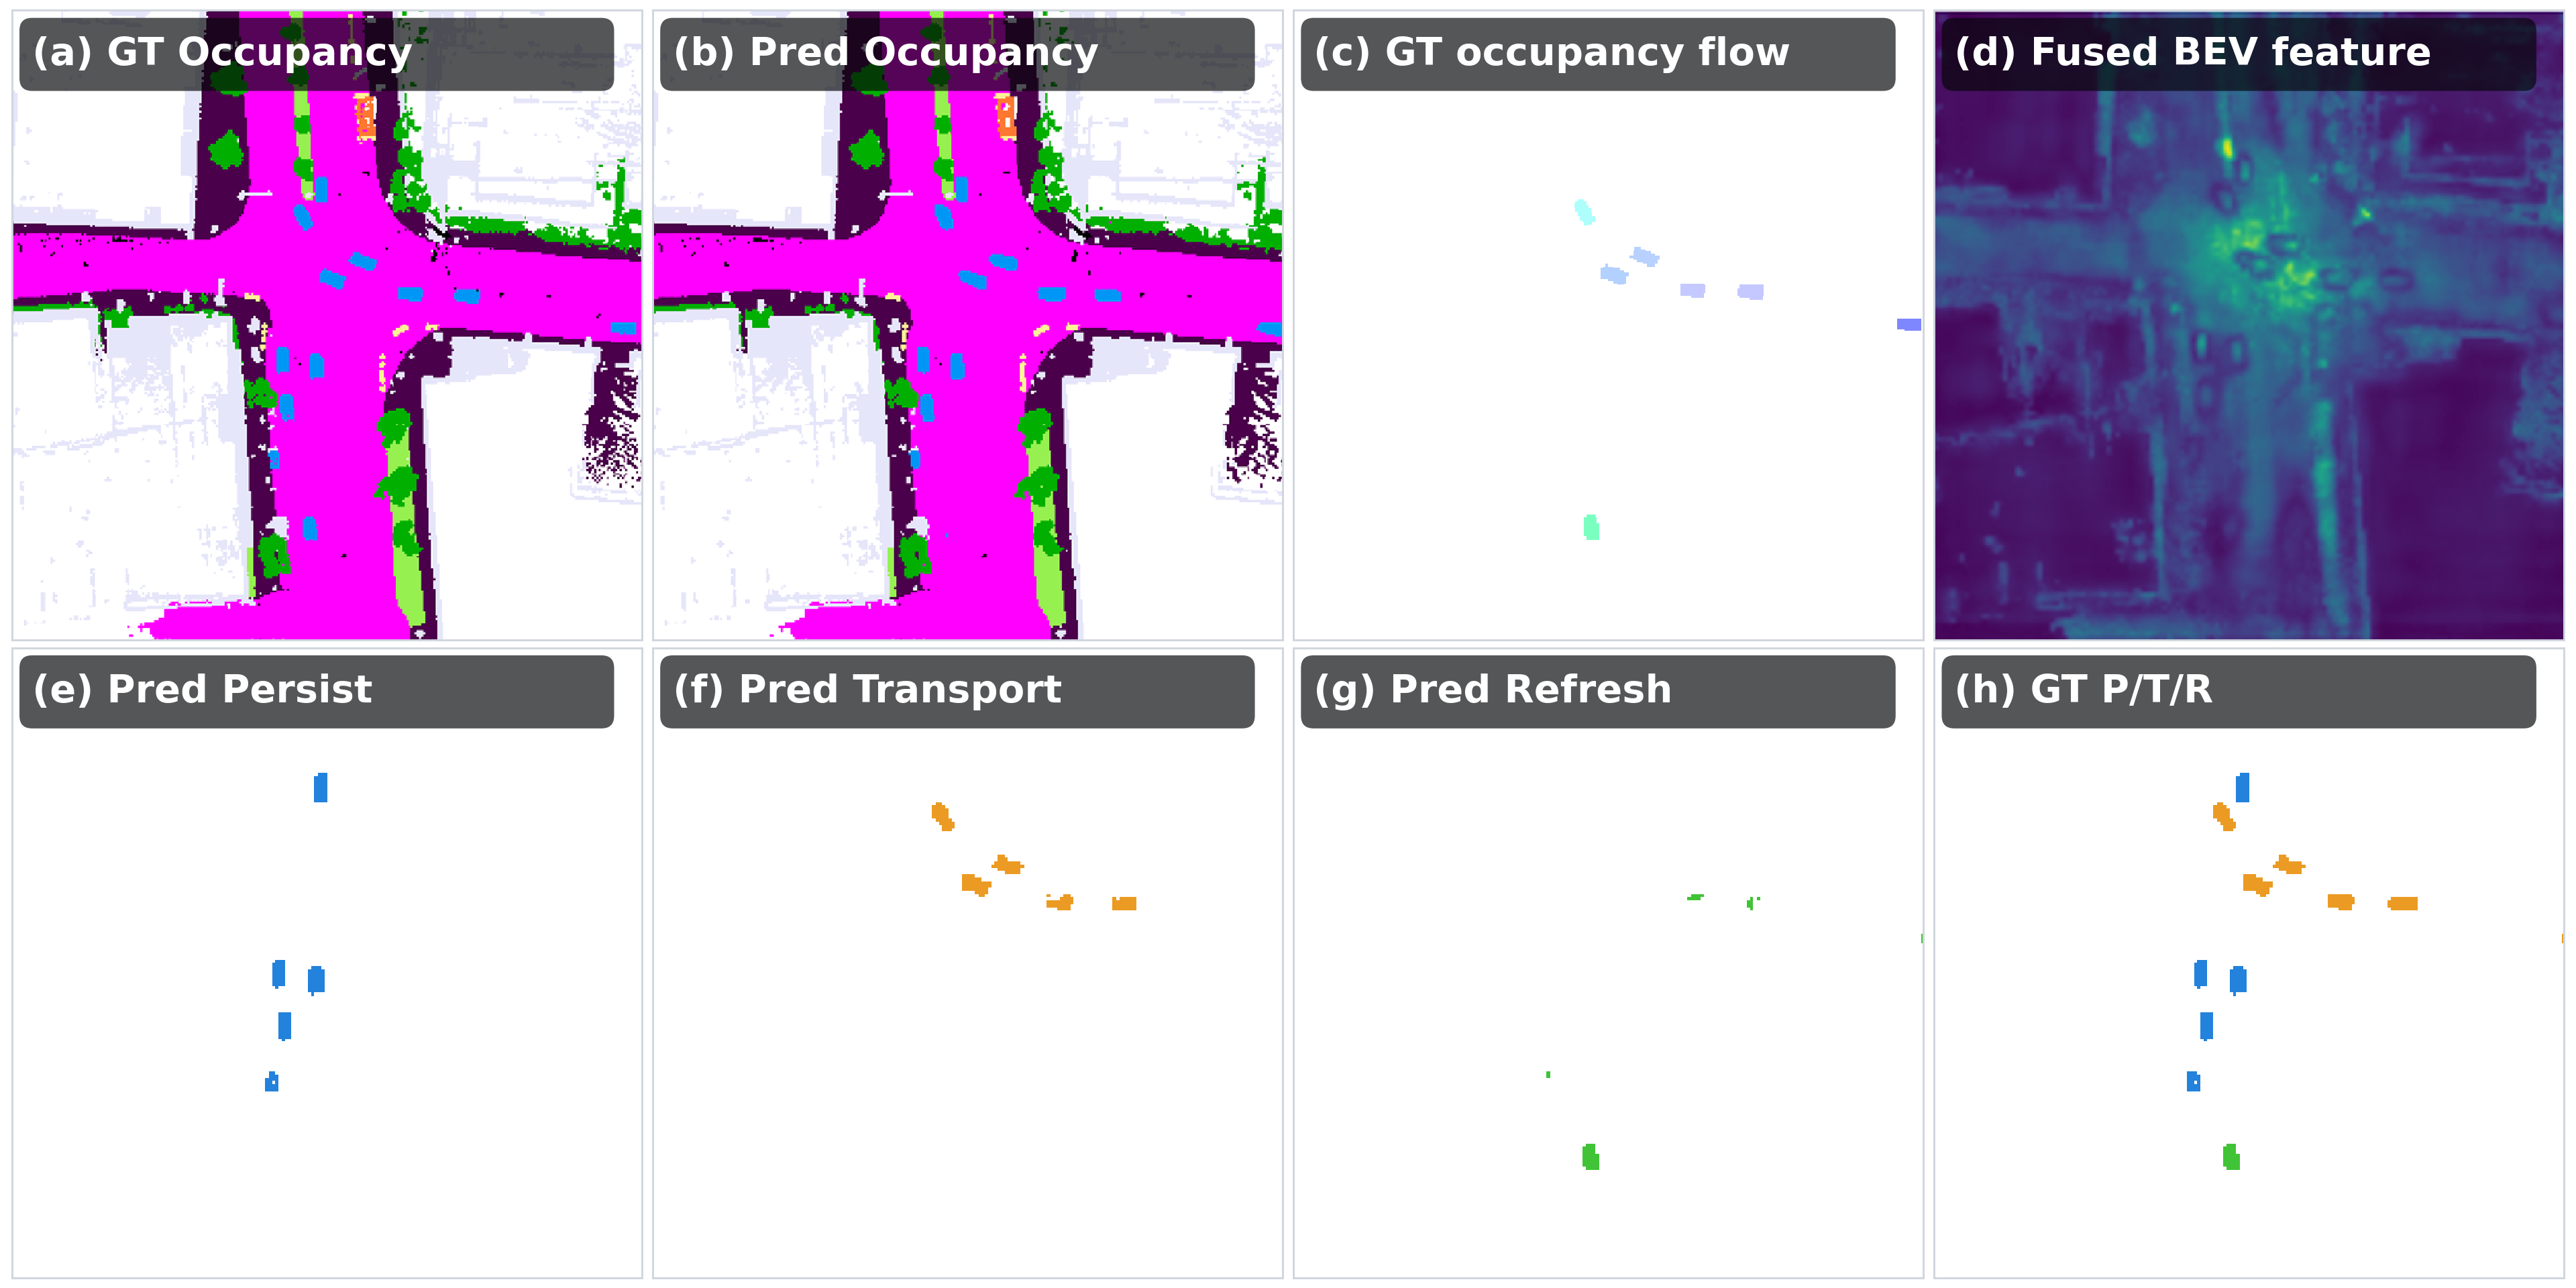
\includegraphics[width=\linewidth]{Fig6-ptrcontrol.png}
  \vspace{-15pt}
  \caption{\textbf{Predicted P/T/R on GT dynamic support.}}
  \vspace{-10pt}
  % Current GT/predicted
  % occupancy, GT flow, and fused BEV features are paired with Persist,
  % Transport, Refresh, and combined routing targets.
  \label{fig:ptr_control}
\end{wrapfigure}
\noindent\textbf{P/T/R source-admissibility routing.}
P/T/R represents semantic source validity rather than instance correspondence.
Persist and Transport require same-class, height-consistent support at the
fixed-coordinate and VVE-addressed locations, while Refresh covers neither
source. GT-conditioned
diagnostics isolate routing from detection, whereas Dyn., Nxt., Direct MAVE, and
DSR retain end-to-end evaluation. This construction turns source validity into
a direct routing decision rather than an implicit feature weight. The supplement
details construction.

\noindent\textbf{Visual analysis.}
Figure~\ref{fig:vve_backwarp} compares zero-motion reading with VVE backtracing.
Current GT fixes the queried dynamic voxels and their classes, while predicted
occupancy provides the end-to-end context. Red-to-green changes show dynamic
flow relocating queries through backwarp sampling onto same-class past GT,
isolating address quality from the subsequent routing decision. On the same GT
dynamic support, Figure~\ref{fig:ptr_control} then shows Persist following
fixed-coordinate support, Transport following displacement, and Refresh
rejecting unsupported history. The paired controls therefore separate where
history is read from which source is selected.

Together, the two visualizations summarize RoadOcc's evidence-routing principle.
VVE resolves \emph{where} each queried voxel should retrieve historical evidence,
while P/T/R verifies its semantic validity, preserving supported history and
refreshing unreliable evidence before VDSF fusion.

\section{Conclusion}
\label{sec:conclusion}

In this work, we present RoadOcc, a voxel-level evidence-source routing framework for temporal
roadside occupancy. Rather than relying on implicit temporal aggregation,
RoadOcc explicitly determines where supported history should be retrieved and
whether it should be reused. DCA uses current image evidence to identify
motion-sensitive voxels, VVE estimates their historical source addresses, and
VDSF turns these addresses into Persist, Transport, or Refresh decisions. On
the InfraOcc protocol, the unified formulation achieves state-of-the-art
occupancy accuracy while improving dynamic recovery and velocity estimation.
Future work will extend this principle to moving platforms, longer temporal horizons, and
instance-level modeling.
% Cross-dataset validation is currently constrained by the absence of another
% compatible real-world benchmark for dense fixed-roadside occupancy. 
% These results support explicit physical
% provenance as a coherent and interpretable complement to conventional temporal
% fusion.
\section*{AI Use Statement}
Generative AI tools were used for literature organization, reviewer-style
feedback, and language editing. The authors verified all citations, technical
descriptions, analyses, and revisions, and take responsibility for the final
content of this work.
\bibliography{iclr2027}
\bibliographystyle{iclr2027}
% Keep the supplementary material in the same single-column ICLR document,
% after the main-paper references.
\clearpage
\onecolumn
\section*{Appendix}

\appendix
% This appendix is input by manuscript.tex after the references.
\providecommand{\method}{RoadOcc}
\providecommand{\metricup}{\ensuremath{\uparrow}}
\providecommand{\metricdown}{\ensuremath{\downarrow}}
\graphicspath{{supplementary/}{./supplementary/}{./}}
\setcounter{figure}{0}
\setcounter{table}{0}
\renewcommand{\thefigure}{A\arabic{figure}}
\renewcommand{\thetable}{A\arabic{table}}

\newcolumntype{C}[1]{>{\centering\arraybackslash}m{#1}}
\newcolumntype{L}[1]{>{\raggedright\arraybackslash}m{#1}}


\section{Overview}
This supplement documents the implementation and controlled evidence underlying
\method{}. (1) Sections~\ref{sec:sensor_setup}--\ref{sec:velocity_target_contract}
define the fixed-roadside data and velocity targets used to construct historical
addresses. (2) Section~\ref{sec:metrics} specifies the coupled occupancy,
motion, and coverage diagnostics used to assess those addresses and their routed
sources. (3) Sections~\ref{sec:training_objectives}--\ref{sec:exact_contract}
provide the scale-wise objectives and exact DCA--VVE--VDSF execution contract.
(4) Sections~\ref{sec:model_size}--\ref{sec:visuals} report efficiency,
controlled studies, and scope under the complete model configuration.

\section{Roadside Sensor Configuration}
\label{sec:sensor_setup}

\begin{wrapfigure}{r}{0.50\columnwidth}
  \centering
  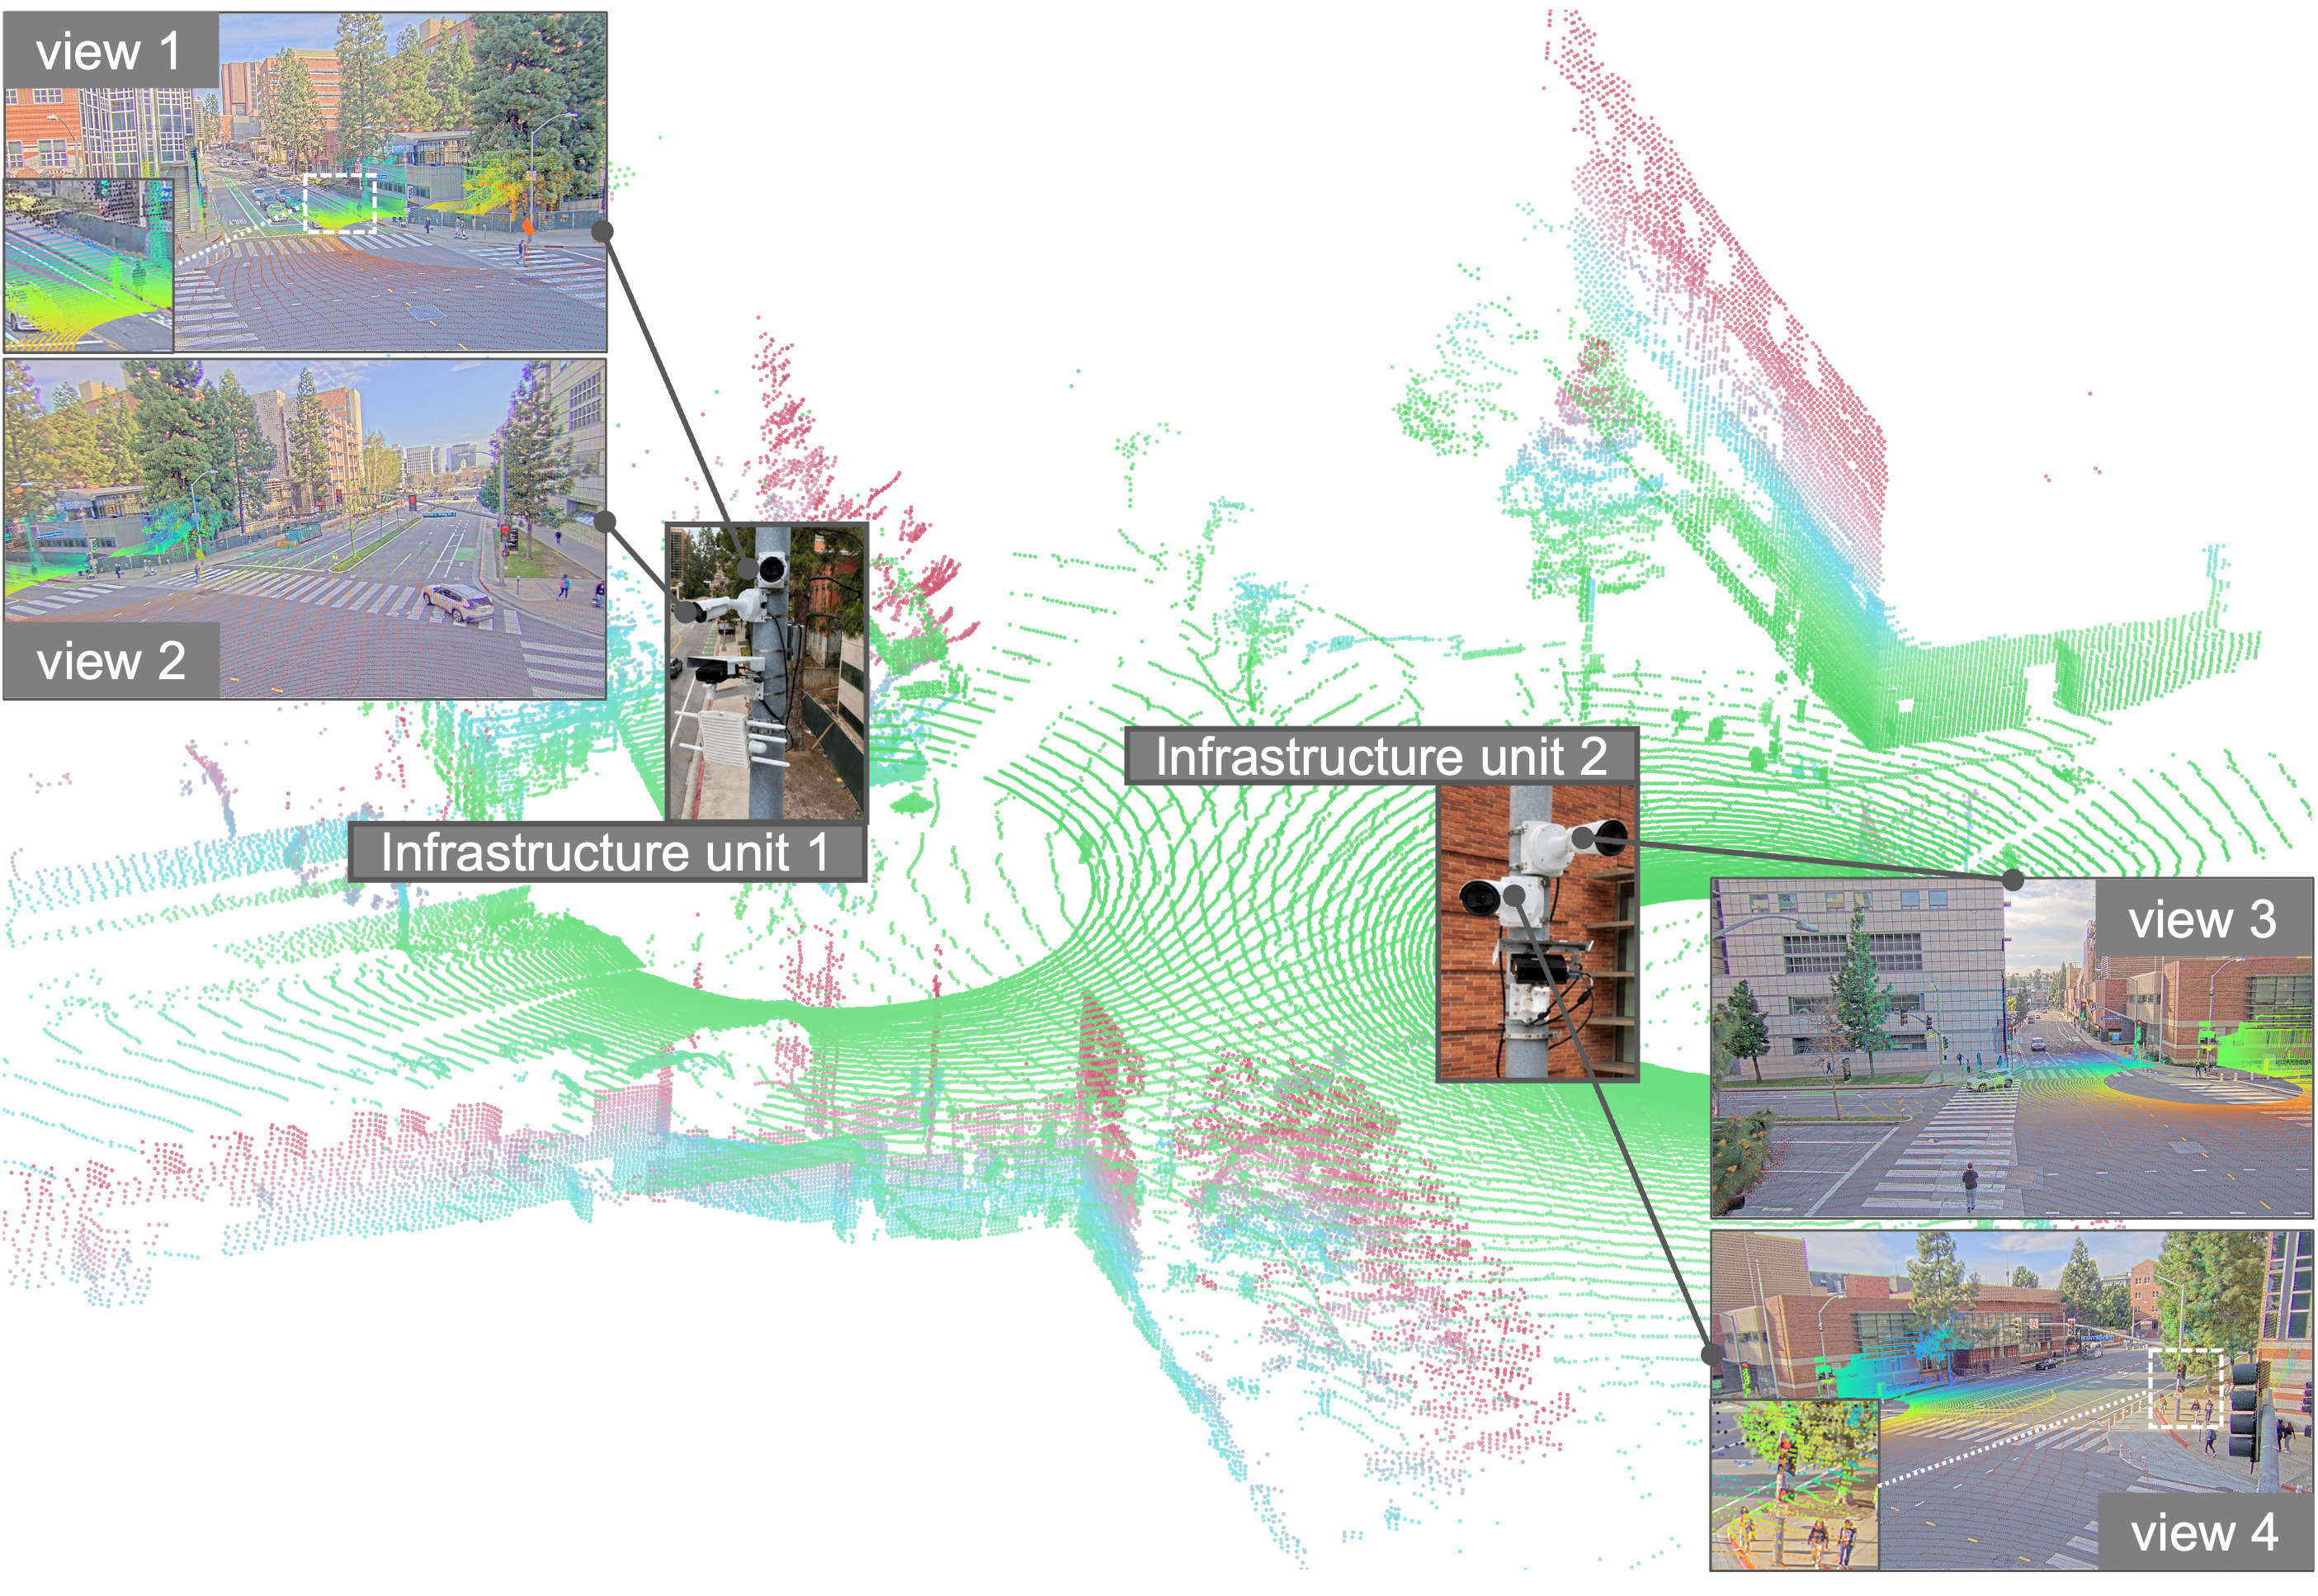
\includegraphics[width=\linewidth]{Fig1-sensor-setup.png}
  \caption{Infrastructure-side sensor configuration. Two fixed units provide
  four synchronized cameras and two LiDARs calibrated to a common roadside
  frame.}
  \vspace{-10pt}
  \label{fig:sensor_setup}
\end{wrapfigure}

InfraOcc reorganizes synchronized V2X-Real streams from object-level
cooperative perception into dense roadside occupancy supervision
\citep{InfraOcc}. Two fixed infrastructure units each carry one LiDAR and two
high-resolution cameras under GPS time synchronization. Calibration maps the
four camera streams, two point clouds, and occupancy annotations into a common
roadside coordinate system. The four cameras are the only exteroceptive model
inputs. LiDAR is used solely for benchmark construction and ground-truth
generation. Thus the reported setting remains camera-only despite the
multimodal data-collection platform.

Roadside benchmarks such as Rope3D and DAIR-V2X also study fixed or cooperative
perception \citep{Rope3D,DAIRV2X}, but primarily evaluate object-level
detection. InfraOcc instead retains a fixed coordinate system for dense
occupancy, exposing voxel-level persistence and displacement. This property is
essential for testing whether a current voxel retrieves its historical feature
from a source-consistent location.

\subsection{Benchmark Scope and Construction Contract}
\label{sec:benchmark_contract}

InfraOcc provides a real-world protocol that combines fixed roadside sensing,
temporally continuous dense semantic voxel labels, and camera-only evaluation.
Ego-centric occupancy benchmarks assume a moving sensor frame, while existing
roadside and cooperative datasets predominantly expose object-level detection
or tracking labels. We therefore use the InfraOcc protocol for primary
evaluation and complement it with matched P/T/R transfer to two temporal
occupancy backbones.

The benchmark contains 290 temporally continuous roadside sequences, with 215
used for training and 75 for evaluation. Each sequence spans approximately
10--24 seconds. Raw streams are captured at 10 Hz and dense occupancy is labeled
at 2 Hz, giving the 0.5 s interval used by RoadOcc. Each keyframe contains four
calibrated camera views and a semantic occupancy volume over
$[-64,64]\times[-64,64]\times[-4.8,1.6]$ m at 0.4 m resolution, or
$320\times320\times16$ voxels. Labels distinguish occupied, free, and
unobserved space; unobserved voxels are excluded from supervision and
evaluation.

Occupancy construction separates persistent structure from transient objects.
A semantic static scaffold is accumulated from registered vehicle-side LiDAR
after dynamic-point removal. Dynamic geometry is reconstructed from
infrastructure-side LiDAR using annotated object tracklets, box-guided alignment,
and local registration. The two sources are recomposed at each keyframe in the
fixed roadside frame and voxelized. Ray traversal labels free space before the
first observed surface, while voxels behind surfaces or outside valid rays remain
unobserved. These LiDAR sources construct supervision only; RoadOcc receives no
LiDAR feature as model input.

\begin{figure}[t]
  \centering
  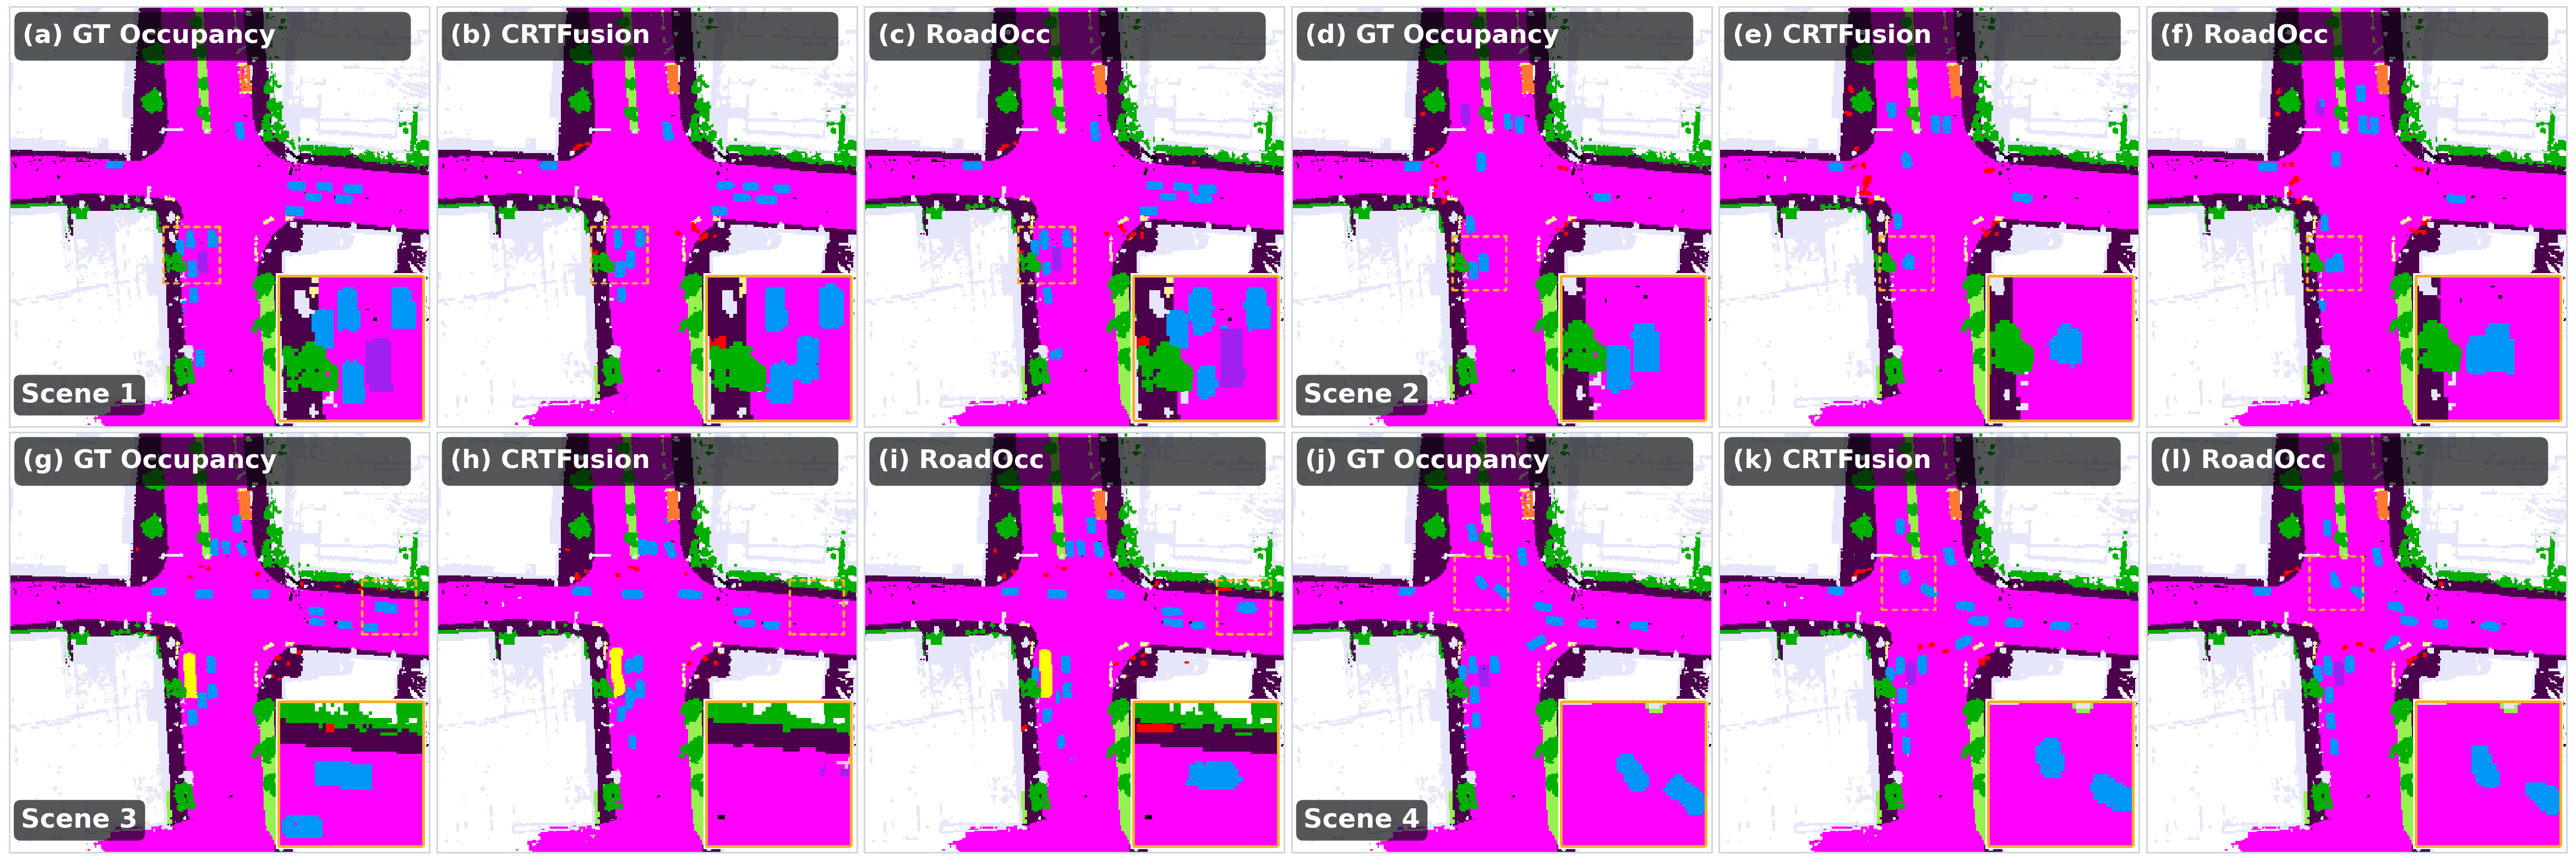
\includegraphics[width=\linewidth]{Fig2-comparison.png}
  \caption{Matched-token occupancy comparison across four scenes. Each triplet
  shows GT, CRT-Fusion, and RoadOcc in a common BEV frame and semantic palette.
  The lower-right insets enlarge a representative region that RoadOcc recovers
  but CRT-Fusion mispredicts.}
  \label{fig:supp_crtfusion}
\end{figure}

\noindent\textbf{Qualitative occupancy recovery.}
Figure~\ref{fig:supp_crtfusion} compares both methods on identical tokens and
coordinates. In the highlighted regions, CRT-Fusion either omits a participant
or assigns an incorrect footprint, whereas RoadOcc more closely follows the GT
extent and class. The surrounding road structure remains visually unchanged.
The gain is therefore concentrated on transient participants rather than
obtained by altering the dominant static background.

\subsection{Velocity-Target Construction}
\label{sec:velocity_target_contract}

InfraOcc occupancy labels do not by themselves define the transport field used
by RoadOcc. We therefore generate planar voxel-velocity targets from annotated
dynamic boxes and their temporal tracklets. Raw box velocity and adjacent-frame
tracklet displacement provide two candidates in the fixed roadside frame.

For track $j$, let $\mathbf R_{\rm rs\leftarrow raw}$ transform planar vectors
from the annotation frame into the fixed roadside frame, and let
$\mathbf c_{j,t}^{\rm rs}$ be its roadside-frame center. The two candidate
velocities are
\begin{equation}
 \widetilde{\mathbf v}_{j,t}
 =\mathbf R_{\rm rs\leftarrow raw}\mathbf v^{\rm raw}_{j,t},
 \qquad
 \mathbf d_{j,t}
 =\frac{\mathbf c_{j,t+\Delta t}^{\rm rs}-\mathbf c_{j,t}^{\rm rs}}{\Delta t},
 \qquad \Delta t=0.5\ \mathrm{s}.
 \label{eq:supp_velocity_candidates}
\end{equation}
We denote the selected candidate by $\overline{\mathbf v}_{j,t}$. A valid
tracklet displacement replaces the raw estimate when the raw estimate is
invalid, when their speeds differ by at most $10\ \mathrm{m/s}$, or when their
speed ratio is at most two.
The corrected velocity is rasterized over dynamic occupancy inside each box,
whose vertical extent is expanded by a factor of 1.5 to absorb sparse boundary
misalignment. Let $\widetilde B_{j,t}$ denote this expanded box. The native
target assigned to a dynamic voxel is
\begin{equation}
 \mathbf v_t^{\rm gt}(\mathbf x)=
 \begin{cases}
 \mathbf 0, & \|\overline{\mathbf v}_{j,t}\|_2<0.8\ \mathrm{m/s},\\
 \operatorname{clip}_{60}\!\left(\overline{\mathbf v}_{j,t}\right),
 & \mathbf x\in\widetilde B_{j,t}\cap\mathcal O_{t}^{\rm dyn},
 \end{cases}
 \label{eq:supp_velocity_rasterization}
\end{equation}
where $\operatorname{clip}_{60}$ limits the magnitude to $60\ \mathrm{m/s}$.
For candidates no faster than 2 m/s, a one-step ($0.5$ s)
future-occupancy check compares zero-motion and transported same-class support.
The check is applied only with at least eight support voxels; zero motion is
selected when its score exceeds the transported score by at least 0.05.
Finally, face-connected component repair propagates valid motion within the
corresponding raw dynamic occupancy component, and targets are generated at
native, $1/2$, $1/4$, and $1/8$ scales.

Future occupancy is used only to construct offline supervision and evaluation
targets. Neither future images nor future features are provided to RoadOcc at
training or inference time. The two velocity thresholds serve different roles.
The 0.8 m/s threshold denoises the physical target, whereas
$\epsilon=10^{-3}$ m/s is the numerical zero test used by the P/T/R rule after
target construction.

\section{Evaluation Contract}
\label{sec:metrics}

Aggregate occupancy is dominated by persistent structure and can therefore
conceal missed or stale traffic participants. Standard protocols emphasize
semantic and geometric IoU \citep{OpenOccupancy,Occ3D2023}, whereas dynamic
occupancy and flow require motion-aware diagnostics
\citep{Cam4DOcc,LetOccFlow}. Table~\ref{tab:supp_metric_contract} formalizes our
evaluation contract on InfraOcc \citep{V2XReal,InfraOcc}. Dynamic and next-frame
IoU measure semantic recovery at the current and flow-advected next-frame
locations. Direct MAVE
and DSR jointly measure motion accuracy and coverage. Static, geometric, and ray
metrics measure whether dynamic recovery preserves the fixed scene. Together,
these diagnostics distinguish improved correspondence from reduced dynamic
support or retained stale evidence.

\begin{figure*}[t]
  \centering
  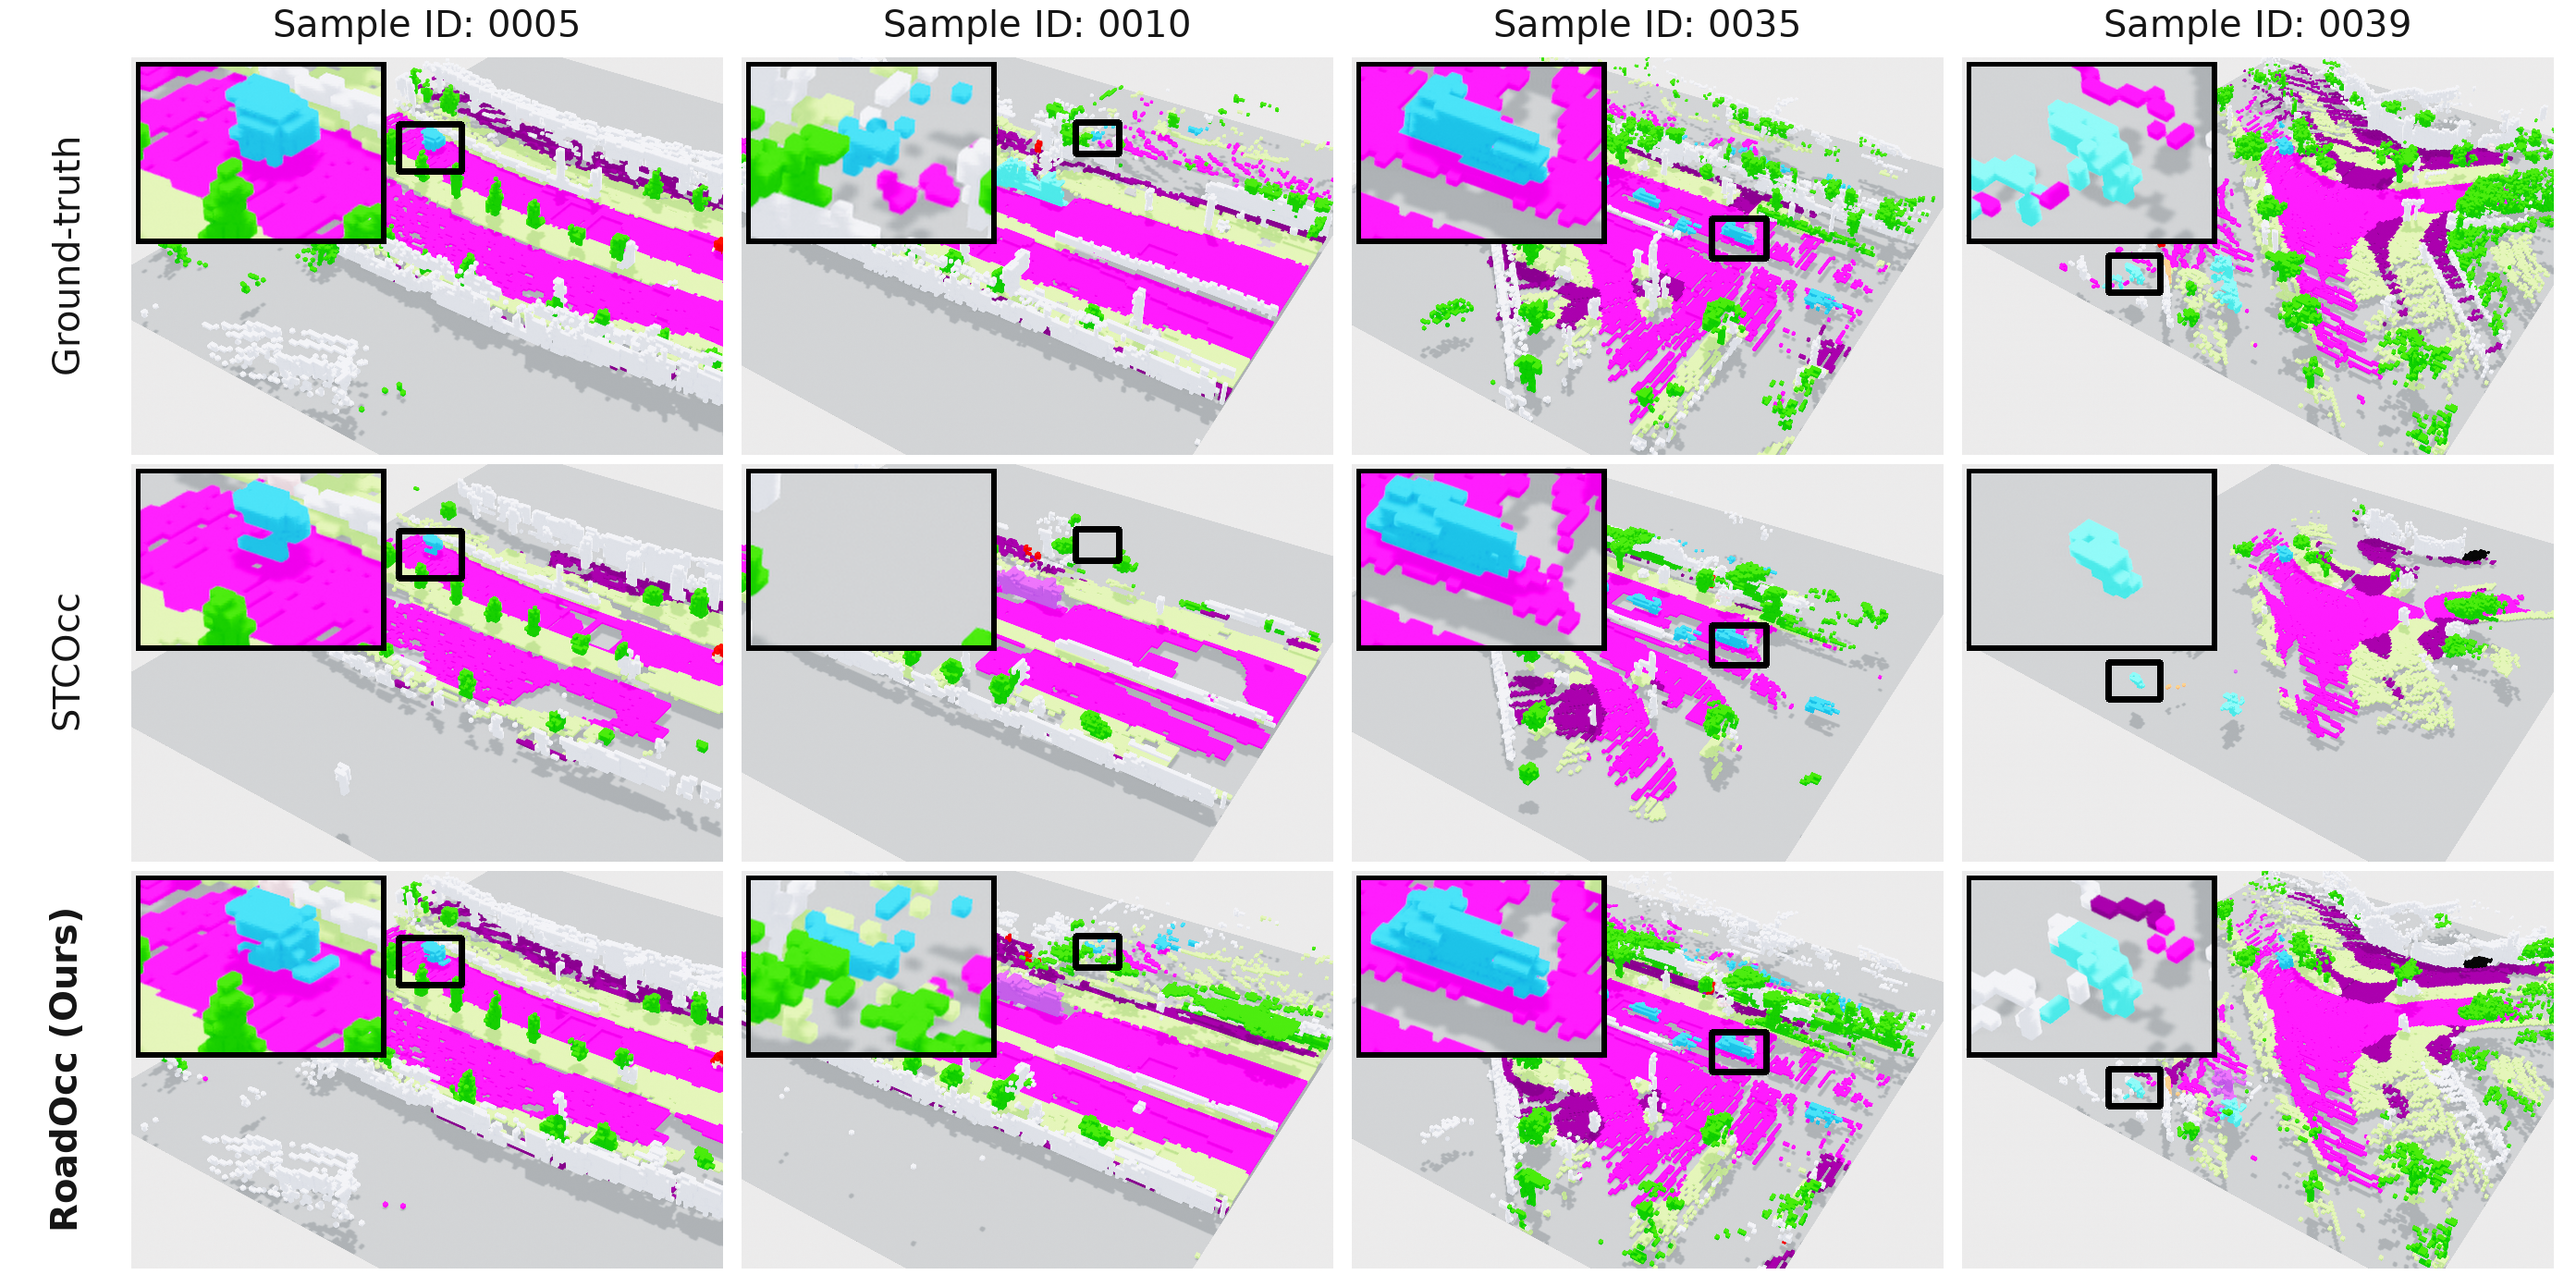
\includegraphics[width=\textwidth]{supplementary/Fig3-occ3d-comparison.png}
  \caption{\textbf{Qualitative comparison on Occ3D-nuScenes.}
  We show four validation frames under the official camera-visible mask,
  semantic palette, voxel grid, and viewing transform. Black boxes and the
  upper-left insets show the same GT dynamic component in all three rows.
  Each region is selected where RoadOcc recovers more of that component than
  the released STCOcc checkpoint.}
  \label{fig:supp_occ3d_comparison}
\end{figure*}

\noindent\textbf{Dynamic-object comparison.}
From left to right, RoadOcc raises recall within the highlighted GT component
from 58.5 to 92.5, 0.0 to 87.5, 76.4 to 92.7, and 59.0 to 90.2\%, respectively.
The insets show the corresponding recovery of missed or truncated traffic
participants.

\begin{table}[h]
  \belowrulesep=0pt
  \aboverulesep=0pt
  \centering
  \footnotesize
  \caption{Metric and diagnostic scope.}
  \label{tab:supp_metric_contract}
  \renewcommand{\arraystretch}{1.05}
  \setlength{\tabcolsep}{0pt}
  \begin{tabular*}{\textwidth}{@{\extracolsep{\fill}}llll@{}}
    \toprule[1.0pt]
    \multicolumn{1}{c}{Metric} & \multicolumn{1}{c}{Support} &
    \multicolumn{1}{c}{Failure} & \multicolumn{1}{c}{Role} \\
    \midrule
    Dyn. mIoU $\metricup$ & Dynamic GT voxels & Omission / class error & Dynamic semantic recovery \\
    Static / gIoU $\metricup$ & Static / occupied support & Static-structure damage & Static-scene guardrail \\
    Next Dyn. $\metricup$ & Advected dynamic GT & Displacement error & Next-frame consistency \\
    Direct MAVE $\metricdown$ & All dynamic GT voxels & Miss-induced motion bias & Unconditional flow error \\
    TP-MAVE $\metricdown$ / DSR $\metricup$ & Matched semantics / dynamic GT & Conditional-match bias & Matched accuracy / coverage \\
    RayIoU $\metricup$ & Visible evaluation rays & Surface-depth mismatch & Geometric fidelity \\
    \bottomrule
  \end{tabular*}
\end{table}



Direct MAVE evaluates every valid GT dynamic voxel, whereas TP-MAVE is
conditional on a correct semantic match and must therefore be interpreted with
DSR. A valid routing improvement should increase dynamic IoU and DSR, decrease
Direct MAVE, and preserve the static and geometric guardrails. Reporting these
quantities together distinguishes improved semantic correspondence from a lower
conditional error caused by reduced semantic support.
For completeness, let $\mathcal D$ be the set of evaluated dynamic classes,
$V_c=\{i:y_i=c\}$ the valid GT voxels of class $c$, and
$V_c^{\rm TP}=\{i\in V_c:\widehat y_i=c\}$. Classes without valid support are
omitted from the corresponding class macro-average; $\mathcal D'$ and
$\mathcal D''$ denote the supported classes for Direct and TP-MAVE,
respectively. The two velocity metrics and semantic recall are
\begin{align}
 \mathrm{Direct\ MAVE}
 &=\frac{1}{|\mathcal D'|}\sum_{c\in\mathcal D'}
   \frac{1}{|V_c|}\sum_{i\in V_c}
   \|\widehat{\mathbf v}_i-\mathbf v_i\|_2,\\
 \mathrm{TP\mbox{-}MAVE}
 &=\frac{1}{|\mathcal D''|}\sum_{c\in\mathcal D''}
   \frac{1}{|V_c^{\rm TP}|}\sum_{i\in V_c^{\rm TP}}
   \|\widehat{\mathbf v}_i-\mathbf v_i\|_2.
\end{align}
Thus MAVE is class-macro while DSR is a micro recall over GT dynamic voxels.
For next-frame dynamic IoU, centers of predicted current dynamic voxels are
advanced by the predicted planar velocity for $0.5$ s, transformed to the next
roadside frame, and voxelized. Collisions use deterministic per-class majority
assignment before class-macro IoU is computed against next-frame GT. This
flow-advected diagnostic is distinct from the same-class radius-one hit score
used only in the backwarp visualization.
\begin{align}
\mathrm{DSR}
&=\frac{\sum_{c\in\mathcal D}|V_c^{\rm TP}|}
        {\sum_{c\in\mathcal D}|V_c|}.
\end{align}



\section{Occ3D-nuScenes Transfer}
\label{sec:occ3d_nuscenes}

\begin{wraptable}[11]{r}{0.62\columnwidth}
  \vspace{-5pt}
  \belowrulesep=0pt
  \aboverulesep=0pt
  \centering
  \footnotesize
  \caption{Mask-trained comparison on Occ3D-nuScenes. All metrics are percentages.}
  \label{tab:occ3d_nuscenes}
  \setlength{\tabcolsep}{0pt}
  \renewcommand{\arraystretch}{1.05}
  \begin{tabular}{@{}C{2.40cm}C{1.10cm}C{1.35cm}C{0.80cm}C{1.55cm}C{1.45cm}@{}}
    \toprule
    Method & BB & Res. & mIoU & Dynamic mIoU & Static mIoU \\
    \midrule
    FB-Occ & R50 & 256$\!\times\!$704 & 39.10 & 33.75 & 43.89 \\
    ViewFormer & R50 & 256$\!\times\!$704 & 41.90 & 35.00 & 47.93 \\
    COTR & R50 & 256$\!\times\!$704 & 44.50 & 38.60 & 49.63 \\
    ALOcc & R50 & 256$\!\times\!$704 & 41.40 & 35.40 & 46.73 \\
    STCOcc & R50 & 256$\!\times\!$704 & 44.60 & 39.01 & 49.58 \\
    \method{} & R50 & 256$\!\times\!$704 & \textbf{45.01} & \textbf{39.80} & \textbf{49.64} \\
    \bottomrule
  \end{tabular}
\end{wraptable}

Table~\ref{tab:occ3d_nuscenes} compares representative camera-only temporal
methods under the mask-trained Occ3D-nuScenes protocol~\citep{Occ3D2023,FBOCC,ALOcc,ViewFormer,COTR,STCOcc}.
Dynamic mIoU averages the eight traffic-participant classes, while static mIoU
averages the remaining nine occupied classes. We compute both group metrics
from published per-class IoUs when available. ALOcc directly reports dynamic
mIoU; its static mIoU follows from its reported dynamic and overall mIoUs.
Before rounding, the three aggregates satisfy
$\mathrm{mIoU}=(8\,\mathrm{Dyn.}+9\,\mathrm{Sta.})/17$.
RoadOcc leads all three aggregates, improving STCOcc by 0.41 overall, 0.79
dynamic, and 0.06 static mIoU points. The larger dynamic gain shows that
motion-aware routing transfers without sacrificing static-scene accuracy.


\section{Training Objectives}
\label{sec:training_objectives}
\begin{figure}[t]
  \centering
  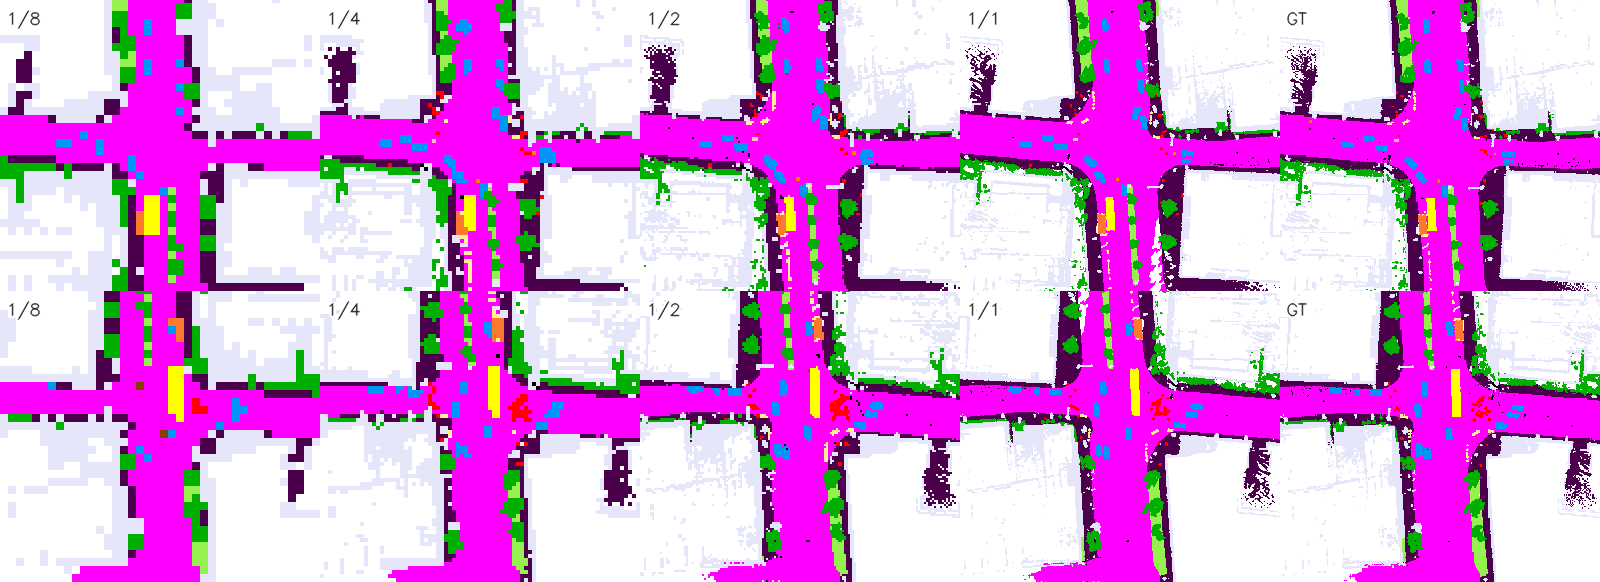
\includegraphics[width=\textwidth]{Fig4-recursive.png}
  \caption{Coarse-to-fine occupancy decoding for two representative samples.
  Columns show predictions from $1/8$ scale through full resolution and the
  corresponding GT. Successive stages sharpen road boundaries and recover
  traffic participants that remain unresolved at coarse resolution.}
  \label{fig:supp_recursive_decoding}
\end{figure}
RoadOcc assigns each loss to one decision in the DCA--VVE--VDSF chain.
Camera-depth supervision uses weight $0.5$. Semantic occupancy is supervised
from full resolution to $1/8$ scale with weights $[1.0,0.5,0.25,0.125]$, while
the static, dynamic, and DCA-candidate auxiliaries each use $0.5$. VVE receives
class- and speed-balanced robust flow supervision at all four scales with weight
$0.1$. Its local-connectivity term also uses $0.1$ and starts after epoch 3 to
limit noisy early correspondences.
The P/T/R route loss spans the native, $1/2$, $1/4$, and $1/8$ scales with
relative weights $[1,0.5,0.25,0.125]$, normalized under
$\lambda_{\rm route}=0.5$. Each scale constructs the semantic-support target
using its physical cell size. Equal-class-weight cross-entropy is augmented from
epoch 2 by a soft-overlap term of weight $0.5$ with state weights
$[1,1,0.25]$. Each executed routing field therefore receives
resolution-matched supervision.


\subsection{Candidate, Motion, and Routing Contract}
\label{sec:exact_contract}

\noindent\textbf{DCA score.}
Let $\boldsymbol\pi_{\rm cur}$ and $\boldsymbol\pi_{\rm sta}$ denote current
and static-reference class probabilities, and let
$\mathcal C_{\rm sta}^{+}$ contain the static classes together with empty
class. The executed
change and dynamic scores are
\begin{align}
 \delta(\mathbf x)&=\frac{1}{|\mathcal C_{\rm sta}^{+}|}
 \sum_{c\in\mathcal C_{\rm sta}^{+}}
 |\pi_{{\rm cur},c}(\mathbf x)-\pi_{{\rm sta},c}(\mathbf x)|,\\
 p_{\rm dyn}(\mathbf x)&=\sum_{c\in\mathcal C_{\rm dyn}}
 \pi_{{\rm cur},c}(\mathbf x),\\
 c(\mathbf x)&=\frac{\max\{\delta(\mathbf x),p_{\rm dyn}(\mathbf x)\}}
 {\max_{\mathbf y}\max\{\delta(\mathbf y),p_{\rm dyn}(\mathbf y)\}+10^{-6}}.
\end{align}
DCA ranks this normalized score. Before fixed top-$K$ selection, VDSF uses
$\operatorname{clip}(c+0.5e,0,1)$, where $e$ is nonempty support and hence
$\eta=0.5$ in Eq.~\ref{eq:vdsf_selection}. For an anchor
$\mathbf r=(\mathbf x,z_{\mathbf r})$, $c(\mathbf r)$ is the score of the
corresponding voxel-height bin and is shared across cameras before visibility
masking. Let $d_{n,\mathbf r}$ be its projected depth, $\widehat d_n$ the
winning predicted depth bin, and $\Delta_d=1$ m the bin width. The executed
depth-consistency factor is
\begin{equation}
 \beta_{n,\mathbf r}=\exp\!\left[-\frac{\sigma^2}{2}
 \min_{\xi\in\{-\Delta_d,+\Delta_d\}}
 \left|d_{n,\mathbf r}-(\widehat d_n+\xi)\right|^2\right],
 \qquad \sigma=2.
\end{equation}
Deformable-attention weights are first softmax-normalized over sampled points,
then multiplied by $\beta$. They are not renormalized afterward; camera
outputs are averaged over cameras retaining at least one visible anchor.




\begin{figure}[t]
  \centering
  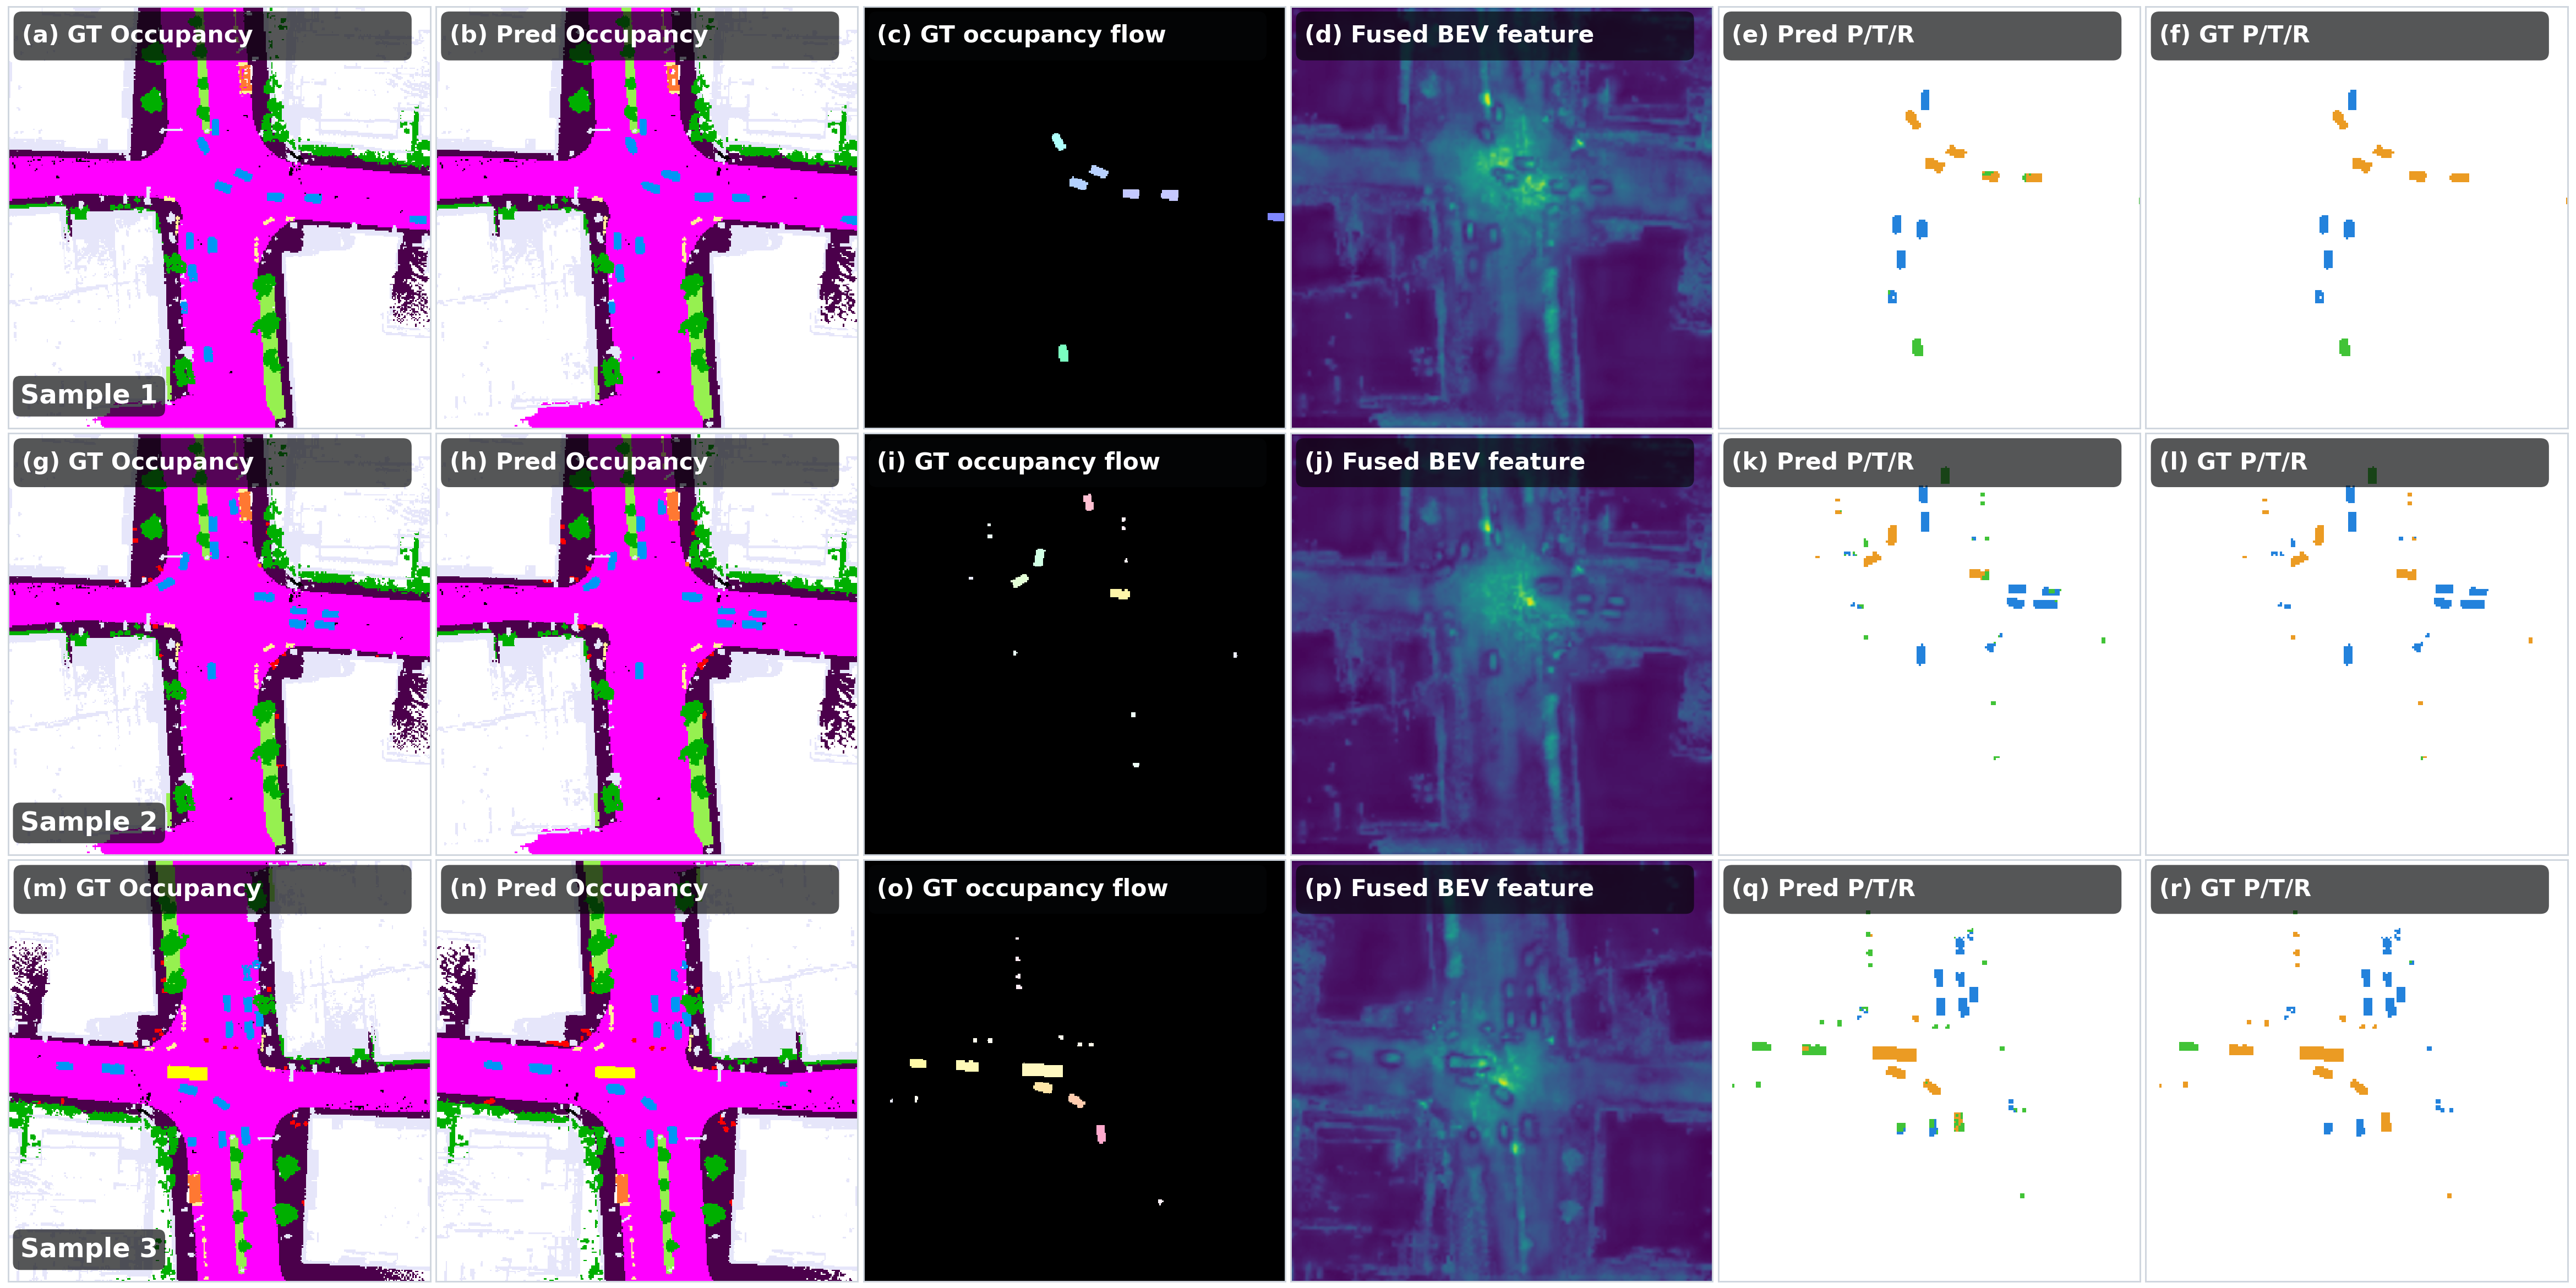
\includegraphics[width=\linewidth]{Fig5-ptrnative.png}
  \caption{Native-scale P/T/R routing across three samples. Predicted and GT
  routes share GT dynamic support. Blue, orange, and green denote Persist,
  Transport, and Refresh, respectively.}
  \label{fig:supp_ptr_prediction}
\end{figure}



\noindent\textbf{Recursive occupancy decoding.}
Figure~\ref{fig:supp_recursive_decoding} shows the progressive output of the
multi-scale decoder. Coarse predictions establish scene layout, while finer
stages restore object boundaries and sparse traffic participants before the
full-resolution output.

\noindent\textbf{VVE correspondence range.}
At scales $1/8$, $1/4$, and $1/2$, the $5\times5$ correlation volume
($r=2$) spans $\pm6.4$, $\pm3.2$, and $\pm1.6$ m on the native $0.4$ m grid.
Over the $0.5$ s interval, the equivalent speed ranges are twice these values.

Each correlation operand is normalized to unit $\ell_2$ norm with
$\epsilon=10^{-6}$. The resulting volume has 25 channels and is concatenated
with current and historical BEV embeddings, processed by two $3\times3$
convolution blocks, and decoded as a two-dimensional velocity residual in m/s.
The window bounds only the
explicit matching evidence. The coarse velocity is
added to each finer prediction and the final continuous residual is not clipped,
so it does not impose a hard bound on predicted speed. The GT-flow study in the
main paper isolates the value of transport addresses across speed ranges. In
the temporal blend, the history branch receives weight
$0.5\,\mathbf 1_{\rm hist}\max_z p_{\rm dyn}(\mathbf x,z)$; this is current
dynamic support gated by history validity, rather than a calibrated measure of
historical correspondence.

\noindent\textbf{Native P/T/R target.}
For a current dynamic voxel, the Transport source is
\begin{equation}
 \mathbf x_{\rm src}=\operatorname{round}\!\left(
 \mathbf x-\frac{\Delta t\,\mathbf v_t(\mathbf x)}{0.4\ \mathrm m}\right),
 \qquad \Delta t=0.5\ \mathrm s.
\end{equation}
Persist tests the fixed-coordinate address and Transport tests $\mathbf x_{\rm src}$.
Support means that the nearest previous GT contains the same semantic class at
the same height within a $3\times3$ XY neighborhood ($L_\infty$ radius one).
Support is Boolean. One or more matching voxels suffice, with no instance-level
tie-breaking.
Out-of-grid or unsupported candidates are assigned Refresh rather than removed.
The target follows InfraOcc's voxel-level semantic supervision and therefore
tests class-consistent support without requiring instance identities.

\noindent\textbf{Coarse-to-fine FIFO routing.}
At each decoder scale, a shared controller projects current features and the
nearest fixed-coordinate history to eight channels, adds embeddings of detached VVE flow
(normalized by 10 m/s) and detached upsampled coarse P/T/R, and predicts three
route logits after a $3\times3\times3$ refinement. A lightweight native head
combines upsampled $1/2$ context, native flow, and the finest P/T/R distribution
for full-resolution routing. Each scale shares its route distribution across
valid FIFO slots, whose ages and cached VVE fields determine source-consistent
inverse-trajectory Transport addresses. Routed slots are concatenated before
fusion. Invalid slots are masked and queues reset at scene boundaries. Fusion
uses soft routes, with argmax only for diagnostics.


\section{Capacity and Efficiency Context}
\label{sec:model_size}

\begin{wraptable}[5]{r}{0.50\columnwidth}
  \vspace{-5pt}
  \belowrulesep=0pt
  \aboverulesep=0pt
  \centering
  \footnotesize
  \caption{Accuracy--efficiency comparison.}
  \label{tab:capacity_efficiency}
  \setlength{\tabcolsep}{2.0pt}
  \renewcommand{\arraystretch}{1.05}
  \begin{tabular}{@{}L{2.20cm}|C{1.00cm}C{1.00cm}|C{1.00cm}C{1.00cm}@{}}
    \toprule[1.0pt]
    Setting & Params.$\downarrow$ & Lat.$\downarrow$ & All$\uparrow$ & Dyn.$\uparrow$ \\
    \midrule
    % BEVDet~'21 & 100.66 & 41.92 & 45.14 & 21.19 \\
    % BEVFormer~'22 & 69.21 & 180.59 & 47.76 & 10.73 \\
    % BEVDepth~'23 & 100.66 & 57.43 & 46.81 & 19.64 \\
    % TPVFormer~'23 & 80.76 & 134.63 & 43.09 & 4.36 \\
    % SurroundOcc~'23 & 80.04 & 44.40 & 50.77 & 11.37 \\
    % CONet~'23 & 100.74 & 53.23 & 49.25 & 18.93 \\
    % SparseOcc~'24 & 105.08 & 64.30 & 45.42 & 9.41 \\
    % GaussianFormer~'24 & 36.32 & 65.50 & 43.63 & 10.45 \\
    % CRT-Fusion~'24 & 56.82 & 106.22 & 53.83 & 27.02 \\
    STCOcc~'25 & 60.47 & 333.44 & 60.85 & 27.66 \\
    RoadOcc (\textbf{ours}) & 78.69 & 253.25 & 65.29 & 32.37 \\
    \bottomrule
  \end{tabular}
  \vspace{-5pt}
\end{wraptable}
Table~\ref{tab:capacity_efficiency} reports parameters, synchronized model
latency measured on a single NVIDIA RTX A6000 with batch size 1, and occupancy
accuracy for the reproduced temporal configurations.
Although RoadOcc contains more parameters than STCOcc, it reduces latency from
333.44 to 253.25 ms because DCA, VVE, and P/T/R operate on sparse or
low-resolution features, while the main temporal path uses shorter histories
and smaller token budgets. This efficient routing also improves all-class and
dynamic mIoU by $+$4.44 and $+$4.71 points, respectively.

\begin{wrapfigure}[17]{r}{0.50\columnwidth}
  \vspace{-15pt}
  \centering
  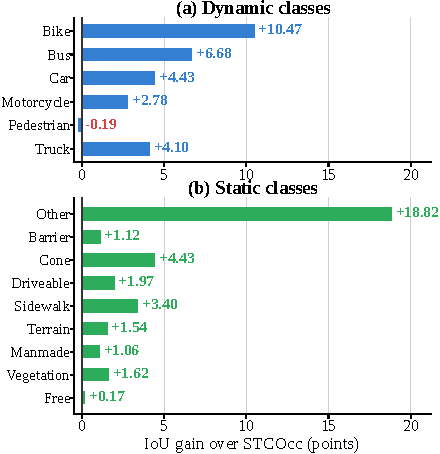
\includegraphics[width=\linewidth]{Fig6-classwise-gains.pdf}
  \caption{Class-wise IoU gains over STCOcc.}
  \label{fig:supp_classwise_gains}
  \vspace{-20pt}
\end{wrapfigure}
\noindent\textbf{Class-wise improvement.}
Figure~\ref{fig:supp_classwise_gains} resolves the official result in
Table~\ref{tab:infraocc_main_results} into dynamic and static classes. Relative
to STCOcc, RoadOcc improves five of the six dynamic classes, led by Bike at
$+$10.47 and Bus at $+$6.68, while Pedestrian changes by $-$0.19. Every static
class also improves. The category pattern therefore connects the aggregate gain
to both parts of the routing objective. Corrected addresses recover transient
participants, while source selection preserves the persistent roadside scene.


\section{Controlled Design Studies}
\label{sec:controlled}


All studies hold the backbone, data protocol, optimizer, training schedule,
scene-boundary queue reset, and VDSF configuration fixed. Unless varied explicitly,
the decoder stages use $K=[2000,512,128]$ sparse tokens and retain
$[8,4,2]$ history samples, respectively. The main paper reports the matched
address and P/T/R controls. The supplementary studies below provide
non-overlapping evidence on VVE training, route prediction, sparse allocation,
and address construction.

\noindent\textbf{Temporal-gap zero-shot generalization.}
Table~\ref{tab:supp_temporal_gap} evaluates checkpoints trained only at the
$0.5$ s cadence without fine-tuning. Phase-offset streams retain all 1,970
validation inputs, while the same 1,520 anchors with valid past and future
$1.5$ s context are scored at every gap. The elapsed time is recovered from
timestamps and used by temporal transport.

\begin{table}[H]
  \belowrulesep=0pt
  \aboverulesep=0pt
  \centering
  \footnotesize
  \caption{Temporal-gap zero-shot evaluation on matched anchors. Both
  checkpoints are trained only at a $0.5$ s interval.}
  \label{tab:supp_temporal_gap}
  \renewcommand{\arraystretch}{1.05}
  \setlength{\tabcolsep}{5.5pt}
  \begin{tabular}{@{}lccc|ccc@{}}
    \toprule[1.0pt]
    & \multicolumn{3}{c|}{Dyn. $\metricup$} &
      \multicolumn{3}{c}{Nxt. $\metricup$} \\
    \cmidrule(lr){2-4}\cmidrule(l){5-7}
    Method & $0.5$ s & $1.0$ s & $1.5$ s & $0.5$ s & $1.0$ s & $1.5$ s \\
    \midrule
    STCOcc~\citep{STCOcc} & 28.04 & 28.26 & 28.58 & 25.21 & 20.90 & 19.12 \\
    RoadOcc (\textbf{ours}) & \textbf{33.71} & \textbf{33.57} & \textbf{33.49} &
      \textbf{30.23} & \textbf{25.18} & \textbf{22.78} \\
    \bottomrule
  \end{tabular}
\end{table}

RoadOcc preserves a 4.91-point Dyn. advantage and a 3.65-point Nxt. advantage
even when the test gap triples. VVE represents displacement through a physical
velocity field, while P/T/R selects fixed-coordinate, transported, or current
evidence. Their combination therefore remains effective when elapsed time
changes rather than depending only on the observed $0.5$ s transition pattern.


\begin{wrapfigure}{r}{0.50\columnwidth}
  \centering
  \vspace{-10pt}
  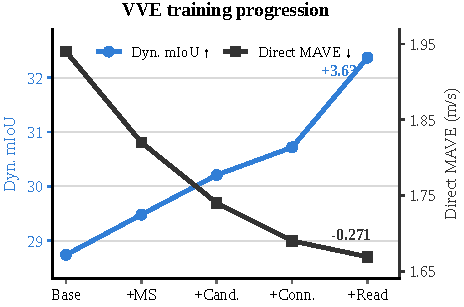
\includegraphics[width=\linewidth]{Fig7-vve-progression.pdf}
  \caption{Dynamic occupancy and motion-error progression under the VVE
  training signals.}
  \label{fig:supp_vve_progression}
  \vspace{-15pt}
\end{wrapfigure}
\noindent\textbf{VVE training design.}
The main-paper control establishes the value of reading from a corrected
address. Figure~\ref{fig:supp_vve_progression} follows a progressive sequence
that introduces multi-scale flow, candidate-map guidance, connectivity
regularization, and flow-addressed history retrieval. Dyn. improves monotonically
while Direct MAVE decreases across this progression. Overall, Dyn. rises by
$+$3.63 and Direct MAVE falls by 0.271. The final flow-addressed read contributes
another $+$1.65 Dyn. while Direct MAVE decreases by only 0.021, indicating that
its main benefit comes from retrieving useful history.

\noindent\textbf{Supported-route analysis.}
Table~\ref{tab:supp_ptr_fidelity} audits the two historical routes on valid GT
dynamic voxels. Persist emphasizes precise reuse of fixed-coordinate evidence,
while Transport provides broader coverage after displacement. Since VDSF fuses
soft probabilities over all source alternatives, these argmax statistics
characterize history reuse rather than the complete fused output. The end-to-end
effect of routing is evaluated separately through Dyn., Nxt., Direct MAVE, and
DSR.

\begin{wraptable}{r}{0.50\columnwidth}
  \belowrulesep=0pt
  \aboverulesep=0pt
  \centering
  \footnotesize
  \caption{Supported historical-route statistics on valid GT dynamic voxels.
  Percentages are computed against the full routing population.}
  \label{tab:supp_ptr_fidelity}
  \renewcommand{\arraystretch}{1.05}
  \setlength{\tabcolsep}{2.2pt}
  \begin{tabular}{@{}L{1.30cm}|C{1.25cm}C{1.25cm}|C{1.25cm}C{1.25cm}@{}}
    \toprule[1.0pt]
    State & Target & Pred. & Precision & Recall \\
    \midrule
    Persist   & 52.34 & 38.84 & 95.50 & 70.87 \\
    Transport & 44.30 & 50.40 & 72.98 & 83.03 \\
    % Refresh   &  3.36 & 10.76 & 16.87 & 54.00 \\
    \bottomrule
  \end{tabular}
  \belowrulesep=0pt
  \aboverulesep=0pt
  \centering
  \footnotesize
  \caption{Sensitivity to sparse-token allocation.}
  \label{tab:supp_token_budget}
  \renewcommand{\arraystretch}{1.05}
  \setlength{\tabcolsep}{0pt}
  \begin{tabular}{@{}C{2.50cm}|C{1.05cm}C{1.05cm}C{1.25cm}C{1.05cm}@{}}
    \toprule[1.0pt]
    Budget $K$ & Dyn. $\metricup$ & Nxt. $\metricup$ & dM $\metricdown$ & DSR $\metricup$ \\
    \midrule
    $[1000,256,64]$ & 31.74 & 30.96 & 1.716 & 60.28 \\
    $[2000,512,128]$ & 32.37 & 31.72 & 1.669 & 61.11 \\
    $[4000,1024,256]$ & 32.39 & 31.69 & 1.665 & 61.18 \\
    \bottomrule
  \end{tabular}
  \vspace{-5pt}
\end{wraptable}
\noindent\textbf{Qualitative routing behavior.}
Figure~\ref{fig:supp_ptr_prediction} relates each route to observable scene
evidence. Persist coincides with aligned objects, Transport follows nonzero
displacement, and current evidence is selected when neither historical source
is supported. Because predicted and GT routes are rendered on identical dynamic
support, their differences directly reflect source choices. The visualization
therefore audits semantic source routing independently of occupancy detection.



\noindent\textbf{Sparse-token budget.}
VDSF processes only the top-$K$ selected voxels. The token study tests whether
the reported behavior depends on a larger compute budget or on identifying the
right locations. All other model and routing settings remain fixed while $K$ is
scaled at every decoder stage.
Increasing the small allocation to the default improves Dyn. by 0.63 and DSR by
0.83. Doubling the default allocation changes Dyn. by only 0.02, dMAVE by 0.004,
and DSR by 0.07, while next-frame IoU fluctuates by $-$0.03. This saturation
shows that the reported result does not rely on continually expanding the
sparse-token budget.



\noindent\textbf{Velocity-address construction.}
Velocity is useful for fusion only when it points to evidence that explains the
current target. Table~\ref{tab:supp_address_rule} therefore compares a
fixed-coordinate read, a target-vector backtrace, and the complete source-consistent
rule under an otherwise fixed P/T/R router. This isolates address construction
from subsequent source acceptance and complements flow-based warping in prior
occupancy models \citep{LetOccFlow,STCOcc}.

\begin{wraptable}{r}{0.50\columnwidth}
  \belowrulesep=0pt
  \aboverulesep=0pt
  \centering
  \footnotesize
  \vspace{-5pt}
  \caption{VVE address control.}
  \label{tab:supp_address_rule}
  \renewcommand{\arraystretch}{1.05}
  \setlength{\tabcolsep}{0pt}
  \begin{tabular}{@{}L{2.50cm}|C{1.10cm}C{1.10cm}C{1.10cm}C{1.10cm}@{}}
    \toprule[1.0pt]
    Address & Dyn. $\metricup$ & Nxt. $\metricup$ & dM $\metricdown$ & DSR $\metricup$ \\
    \midrule
    Ego-aligned read & 30.10 & 29.44 & 2.146 & 57.84 \\
    Target-vector trace & 31.41 & 30.66 & 1.704 & 59.82 \\
    Source-consistent & 32.37 & 31.72 & 1.669 & 61.11 \\
    \bottomrule
  \end{tabular}
  \vspace{-5pt}
\end{wraptable}

Target-vector backtracing improves Dyn. by 1.31 and reduces dMAVE by 0.442 over
the ego-aligned read. Enforcing source consistency contributes a further 0.96
Dyn., 1.06 Nxt., and 1.29 DSR while reducing dMAVE by 0.035. The paired occupancy
and coverage gains show that the refined address is useful for retrieval rather
than only for velocity regression.

\noindent\textbf{Stepwise address benefit.}
Figure~\ref{fig:supp_address_profile} makes the controlled progression in
Table~\ref{tab:supp_address_rule} explicit. Target-vector tracing corrects
motion-aware retrieval, while source consistency adds a further gain by ensuring
that the transported source remains semantically admissible for the current
voxel. Across the full progression, Dyn., Next Dyn., and DSR rise by 2.27, 2.28,
and 3.27 points, respectively, while Direct MAVE falls by 0.477.

\begin{figure}[t]
  \centering
  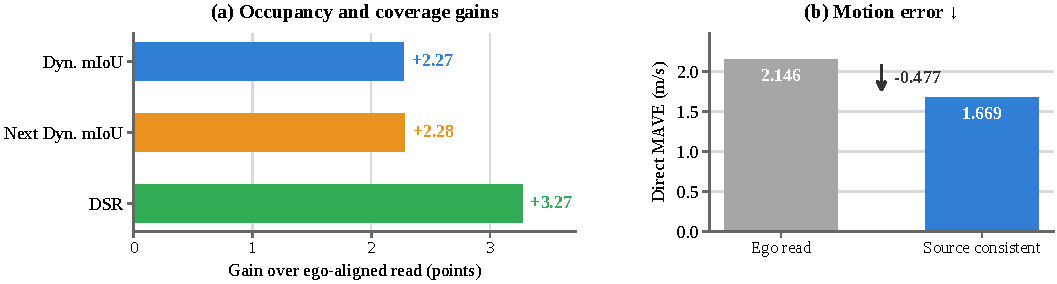
\includegraphics[width=\textwidth]{Fig8-address-benefit.pdf}
  \caption{Measured advantage of source-consistent address construction over
  ego-aligned reading. Values are derived from the matched controlled settings
  in Table~\ref{tab:supp_address_rule}.}
  \label{fig:supp_address_profile}
\end{figure}

\section{Implementation and Scope}
\label{sec:visuals}

The production configuration uses four cameras, a ResNet-50 backbone, three
decoder stages, a $0.4$ m voxel grid, and a $0.5$ s sampling interval. Models are
optimized with AdamW for 24 epochs. Controlled variants share the same
initialization policy, optimizer, schedule, scene-boundary queue reset, and
InfraOcc evaluator. Only the designated factor is changed.

P/T/R operates on semantic voxel support, matching the InfraOcc label space.
Nearby same-class objects can share support within the local radius; when
history has no supported source, Refresh uses the current-frame feature. The
route target therefore encodes semantic evidence admissibility rather than
instance identity. We report dynamic IoU, Direct MAVE, and DSR jointly so that
semantic recovery, motion error, and support coverage remain visible beyond the
GT-conditioned route diagnostic.


\end{document}
